% =====================================================================================
%  safe_prompt_fields.tex
%
%  Distilled version of flow_matching_safe_set_POC.tex, reorganised around one idea:
%  the velocity field of a new prompt is constrained to the order-1 Wasserstein conformal
%  region built from the fields of safe prompts, for flow-matching models that are linear
%  in their parameters.  The original note is kept unchanged as the full record.
%  Build (from this folder):
%      pdflatex safe_prompt_fields && bibtex safe_prompt_fields
%      && pdflatex safe_prompt_fields && pdflatex safe_prompt_fields
%  Every number in Section 7 is copied from tables/numbers.tex and tables/tab_*.tex
%  (written by code/make_tables.py from results/).
% =====================================================================================
\documentclass{article}
\usepackage[preprint]{custom_2020}
\usepackage{amsmath}
\usepackage{stmaryrd}
\usepackage{tgtermes}
\usepackage[dvipsnames]{xcolor}
\usepackage{bm}
\usepackage{bbm}
\usepackage[hidelinks]{hyperref}
\usepackage{amssymb,amsfonts}
\usepackage{caption}
\usepackage{graphicx}
\usepackage{booktabs}
\usepackage{mathtools}
\usepackage{enumitem}
\usepackage{placeins}

\DeclareMathOperator*{\argmin}{arg\,min}
\DeclareMathOperator{\E}{\mathbb{E}}
\DeclareMathOperator{\dist}{dist}
\DeclareMathOperator{\conv}{conv}
\newcommand{\RR}{\mathbb{R}}
\newcommand{\PP}{\mathbbm{P}}
\newcommand{\cD}{\mathcal{D}}
\newcommand{\cE}{\mathcal{E}}
\newcommand{\cL}{\mathcal{L}}
\newcommand{\cN}{\mathcal{N}}
\newcommand{\bth}{\boldsymbol{\theta}}
\newcommand{\bx}{\mathbf{x}}
\newcommand{\by}{\mathbf{y}}
\newcommand{\bu}{\mathbf{u}}
\newcommand{\bb}{\mathbf{b}}
\newcommand{\ba}{\mathbf{a}}
\newcommand{\be}{\mathbf{e}}
\newcommand{\bxi}{\boldsymbol{\xi}}
\newcommand{\TV}{\mathrm{TV}}
\newcommand{\KL}{\mathrm{KL}}
\newcommand{\kl}{\mathrm{kl}}
\newcommand{\Tbar}{\bar{\Theta}}
\newcommand{\vstar}{v^{\star}}

\usepackage{natbib}
 \bibpunct[, ]{(}{)}{,}{a}{}{,}%
 \def\bibfont{\small}%
 \def\bibsep{\smallskipamount}%
 \def\bibhang{24pt}%
 \def\newblock{\ }%
 \def\BIBand{and}%

\usepackage{amsthm}
\theoremstyle{plain}
\newtheorem{theorem}{Theorem}[section]
\newtheorem{lemma}[theorem]{Lemma}
\newtheorem{proposition}[theorem]{Proposition}
\newtheorem{corollary}[theorem]{Corollary}
\newtheorem{definition}[theorem]{Definition}
\newtheorem{assumption}[theorem]{Assumption}
\theoremstyle{remark}
\newtheorem{remark}[theorem]{Remark}

\setlist{itemsep=1pt,topsep=3pt}
\newcommand{\eoneSafePAA}{0.0024}
\newcommand{\eoneZetaA}{1.93}
\newcommand{\eonePAAa}{0.005}
\newcommand{\eonePAAb}{0.014}
\newcommand{\eonePAAc}{0.074}
\newcommand{\eonePAAd}{0.253}
\newcommand{\eoneSafePAB}{0.0046}
\newcommand{\eoneZetaB}{0.26}
\newcommand{\eonePABa}{0.007}
\newcommand{\eonePABb}{0.015}
\newcommand{\eonePABc}{0.065}
\newcommand{\eonePABd}{0.237}
\newcommand{\eoneTruePAd}{0.284}
\newcommand{\eoneOneStepPA}{0.0176}
\newcommand{\eoneCovAT}{0.897}
\newcommand{\eoneExATb}{0.07}
\newcommand{\eoneExATc}{0.24}
\newcommand{\eoneExATd}{1.00}
\newcommand{\eoneBudgetAT}{0.83}
\newcommand{\eoneCovAZ}{0.900}
\newcommand{\eoneExAZb}{0.20}
\newcommand{\eoneExAZc}{0.82}
\newcommand{\eoneExAZd}{0.95}
\newcommand{\eoneBudgetAZ}{0.50}
\newcommand{\eoneCovAR}{0.900}
\newcommand{\eoneExARb}{0.09}
\newcommand{\eoneExARc}{0.16}
\newcommand{\eoneExARd}{0.48}
\newcommand{\eoneBudgetAR}{0.98}
\newcommand{\eoneCovAE}{0.907}
\newcommand{\eoneExAEb}{0.12}
\newcommand{\eoneExAEc}{0.29}
\newcommand{\eoneExAEd}{1.00}
\newcommand{\eoneBudgetAE}{1.61}
\newcommand{\eoneCovBT}{0.900}
\newcommand{\eoneExBTb}{0.10}
\newcommand{\eoneExBTc}{0.29}
\newcommand{\eoneExBTd}{1.00}
\newcommand{\eoneBudgetBT}{0.68}
\newcommand{\eoneCovBZ}{0.901}
\newcommand{\eoneExBZb}{0.10}
\newcommand{\eoneExBZc}{0.29}
\newcommand{\eoneExBZd}{1.00}
\newcommand{\eoneBudgetBZ}{0.58}
\newcommand{\eoneCovBR}{0.900}
\newcommand{\eoneExBRb}{0.12}
\newcommand{\eoneExBRc}{0.32}
\newcommand{\eoneExBRd}{1.00}
\newcommand{\eoneBudgetBR}{0.63}
\newcommand{\eoneCovBE}{0.907}
\newcommand{\eoneExBEb}{0.12}
\newcommand{\eoneExBEc}{0.29}
\newcommand{\eoneExBEd}{1.00}
\newcommand{\eoneBudgetBE}{1.61}
\newcommand{\eoneLfourUd}{0.03}
\newcommand{\eoneLeightUd}{0.02}
\newcommand{\eoneKnnLtwoc}{0.73}
\newcommand{\eoneKnnLonec}{0.98}
\newcommand{\eoneKnnLfourc}{0.40}
\newcommand{\eoneKnnTruncc}{0.99}
\newcommand{\eoneKnnTailb}{0.29}
\newcommand{\eoneKnnTailCov}{0.918}
\newcommand{\eonePlugFail}{0.4\%}
\newcommand{\eonePlugMax}{3.7}
\newcommand{\eoneMarkovMed}{0.99}
\newcommand{\eoneRegionWorst}{0.189}
\newcommand{\eoneOneStepRectOne}{0.97}
\newcommand{\eoneMmdA}{3.3}
\newcommand{\eoneMmdB}{8.1}
\newcommand{\eoneMmdC}{34.9}
\newcommand{\eoneTwoPAasWritten}{0.142}
\newcommand{\eoneTwoPAtrunc}{0.032}
\newcommand{\eoneTwoMmdAsWritten}{84}
\newcommand{\eoneTwoMmdTrunc}{28}
\newcommand{\eoneTwoMmdNone}{149}
\newcommand{\eoneTwoBudgetUL}{0.84}
\newcommand{\eoneTwoBudgetTrunc}{0.18}
\newcommand{\eoneTwoAttackUL}{0.186}
\newcommand{\eoneTwoAttackLone}{0.054}
\newcommand{\eoneTwoAttackTrunc}{0.051}
\newcommand{\eoneTwoAttackTail}{0.044}
\newcommand{\eoneTwoAttackEU}{1.000}
\newcommand{\eoneTwoAttackEknn}{0.974}
\newcommand{\eoneTwoPlugMin}{8\%}
\newcommand{\eoneTwoPlugMax}{28\%}
\newcommand{\eoneTwoTruncMaxRatio}{1.13}
\newcommand{\eoneTwoLoneMaxRatio}{8.5}
\newcommand{\eoneTwoCertTail}{0.077}
\newcommand{\eoneTwoCertTrunc}{0.29}

% written by code/e1_walkthrough.py
\newcommand{\ewPhi}{10.1}
\newcommand{\ewRho}{1.81}
\newcommand{\ewBudRatioOne}{2.2}
\newcommand{\ewBudRatioTwo}{3.6}
\newcommand{\ewTruePAb}{0.029}
\newcommand{\ewTruePAc}{0.094}
\newcommand{\ewTruePAd}{0.283}
\newcommand{\ewMassA}{0.26}
\newcommand{\ewDispA}{1.1}
\newcommand{\ewDispNotA}{0.16}
\newcommand{\ewZetaOne}{1.81}
\newcommand{\ewOneStepAOne}{96}
\newcommand{\ewZetaTwo}{0.17}
\newcommand{\ewOneStepATwo}{3}
\newcommand{\ewSwitch}{38}
\newcommand{\ewRotA}{33}
\newcommand{\ewAngA}{-22}
\newcommand{\ewRotNear}{1.2}
\newcommand{\ewDLtwoNear}{0.08}
\newcommand{\ewDLoneNear}{0.06}
\newcommand{\ewDTrNear}{0.06}
\newcommand{\ewDTailNear}{0.00}
\newcommand{\ewDLtwoRot}{1.01}
\newcommand{\ewDLoneRot}{0.96}
\newcommand{\ewDTrRot}{0.85}
\newcommand{\ewDTailRot}{0.95}
\newcommand{\ewDLtwoUns}{0.68}
\newcommand{\ewDLoneUns}{0.49}
\newcommand{\ewDTrUns}{0.45}
\newcommand{\ewDTailUns}{0.39}
\newcommand{\ewCovU}{93}
\newcommand{\ewSafeLoU}{0.66}
\newcommand{\ewSafeHiU}{1.02}
\newcommand{\ewExUa}{5}
\newcommand{\ewExUb}{1}
\newcommand{\ewExUc}{7}
\newcommand{\ewExUd}{100}
\newcommand{\ewScUzero}{0.75}
\newcommand{\ewScUone}{0.90}
\newcommand{\ewEpsU}{0.86}
\newcommand{\ewCovK}{88}
\newcommand{\ewExKa}{15}
\newcommand{\ewExKb}{26}
\newcommand{\ewExKc}{100}
\newcommand{\ewExKd}{100}
\newcommand{\ewScKzero}{0.33}
\newcommand{\ewScKone}{1.42}
\newcommand{\ewEpsK}{0.18}
\newcommand{\ewSlicePAa}{0.256}
\newcommand{\ewSlicePAb}{0.141}
\newcommand{\ewSlicePAc}{0.028}
\newcommand{\ewSlicePAd}{0.007}
\newcommand{\ewSlicePAe}{0.002}
\newcommand{\ewSlicePAf}{0.000}
\newcommand{\ewSliceMaxU}{0.19}
\newcommand{\ewSliceMaxK}{0.034}
\newcommand{\ewKapU}{0.23}
\newcommand{\ewKapK}{0.72}
\newcommand{\ewAlphaU}{0.77}
\newcommand{\ewAlphaK}{0.28}
\newcommand{\ewRotSlice}{31}
\newcommand{\ewCertU}{0.99}
\newcommand{\ewCertRU}{1.09}
\newcommand{\ewCertQU}{0.19}
\newcommand{\ewCertPAU}{0.141}
\newcommand{\ewCertK}{0.32}
\newcommand{\ewCertRK}{0.73}
\newcommand{\ewCertQK}{0.08}
\newcommand{\ewCertPAK}{0.028}
\newcommand{\ewCertBudgetK}{0.175}
\newcommand{\ewCertFar}{0}
\newcommand{\ewAtkPrompt}{1.000}
\newcommand{\ewAtkWritten}{0.186}
\newcommand{\ewAtkImproved}{0.051}
\newcommand{\ewAtkEmbNear}{1.07}
\newcommand{\ewAtkEmbMed}{1.28}
\newcommand{\ewAtkScU}{2.3}
\newcommand{\ewAtkScK}{5.6}

% written by code/make_reflow_figure.py
\newcommand{\rfVind}{3.8}
\newcommand{\rfVrefl}{0.002}
\newcommand{\rfCostInd}{6.18}
\newcommand{\rfCostRefl}{0.97}
\newcommand{\rfCurv}{1.44}
\newcommand{\rfDecrease}{5.21}
\newcommand{\rfSum}{5.25}
\newcommand{\rfVmin}{1.6}
\newcommand{\rfVzero}{4.3}
\newcommand{\rfEoneDropped}{0.04}

% written by code/e2_figures.py
\newcommand{\etScEstatic}{0.76}
\newcommand{\etMapMaxEstatic}{0.20}
\newcommand{\etMapEstatic}{25}
\newcommand{\etMapSafeEstatic}{95}
\newcommand{\etWEtop}{0.16}
\newcommand{\etWEtopthree}{0.47}
\newcommand{\etScEadaptive}{1.37}
\newcommand{\etMapMaxEadaptive}{0.06}
\newcommand{\etMapEadaptive}{2}
\newcommand{\etMapSafeEadaptive}{100}
\newcommand{\etScFstatic}{0.77}
\newcommand{\etMapMaxTRstatic}{0.27}
\newcommand{\etMapTRstatic}{27}
\newcommand{\etMapSafeTRstatic}{89}
\newcommand{\etWFtop}{0.59}
\newcommand{\etWFtopthree}{0.87}
\newcommand{\etScFadaptive}{1.57}
\newcommand{\etMapMaxTRadaptive}{0.04}
\newcommand{\etMapTRadaptive}{0}
\newcommand{\etMapSafeTRadaptive}{95}
\newcommand{\etTuneGap}{0.05}
\newcommand{\etTuneRegret}{0.005}
\newcommand{\etNearGap}{0.004}
\newcommand{\etDensEA}{0.16}
\newcommand{\etDensUEA}{0.12}
\newcommand{\etEpsEA}{0.63}
\newcommand{\etEpsUEA}{1.60}
\newcommand{\etDensEB}{0.99}
\newcommand{\etDensUEB}{0.13}
\newcommand{\etEpsEB}{0.22}
\newcommand{\etEpsUEB}{1.57}
\newcommand{\etDensOneE}{0.17}
\newcommand{\etDensFA}{0.20}
\newcommand{\etDensUFA}{0.13}
\newcommand{\etEpsFA}{0.20}
\newcommand{\etEpsUFA}{0.59}
\newcommand{\etDensFB}{1.00}
\newcommand{\etDensUFB}{0.15}
\newcommand{\etEpsFB}{0.08}
\newcommand{\etEpsUFB}{0.58}
\newcommand{\etDensOneF}{0.24}
\newcommand{\etDensPA}{0.21}
\newcommand{\etDensUPA}{0.14}
\newcommand{\etEpsPA}{0.15}
\newcommand{\etEpsUPA}{0.58}
\newcommand{\etDensPB}{1.00}
\newcommand{\etDensUPB}{0.16}
\newcommand{\etEpsPB}{0.07}
\newcommand{\etEpsUPB}{0.57}
\newcommand{\etDensOneP}{0.26}
\newcommand{\etAtkOneES}{1.000}
\newcommand{\etAtkMedOneES}{0.983}
\newcommand{\etEnfOneES}{0.049}
\newcommand{\etMmdOneES}{28}
\newcommand{\etAtkOneEA}{0.976}
\newcommand{\etAtkMedOneEA}{0.920}
\newcommand{\etEnfOneEA}{0.009}
\newcommand{\etMmdOneEA}{11}
\newcommand{\etAtkOnePBS}{0.262}
\newcommand{\etAtkMedOnePBS}{0.131}
\newcommand{\etEnfOnePBS}{0.132}
\newcommand{\etMmdOnePBS}{73}
\newcommand{\etAtkOnePBA}{0.030}
\newcommand{\etAtkMedOnePBA}{0.021}
\newcommand{\etEnfOnePBA}{0.019}
\newcommand{\etMmdOnePBA}{21}
\newcommand{\etAtkOneFS}{0.220}
\newcommand{\etAtkMedOneFS}{0.146}
\newcommand{\etEnfOneFS}{0.077}
\newcommand{\etMmdOneFS}{49}
\newcommand{\etAtkOneFA}{0.036}
\newcommand{\etAtkMedOneFA}{0.020}
\newcommand{\etEnfOneFA}{0.026}
\newcommand{\etMmdOneFA}{26}
\newcommand{\etAtkTwoES}{0.655}
\newcommand{\etAtkMedTwoES}{0.537}
\newcommand{\etEnfTwoES}{0.061}
\newcommand{\etMmdTwoES}{78}
\newcommand{\etAtkTwoEA}{0.496}
\newcommand{\etAtkMedTwoEA}{0.228}
\newcommand{\etEnfTwoEA}{0.027}
\newcommand{\etMmdTwoEA}{47}
\newcommand{\etAtkTwoPBS}{0.099}
\newcommand{\etAtkMedTwoPBS}{0.086}
\newcommand{\etEnfTwoPBS}{0.057}
\newcommand{\etMmdTwoPBS}{89}
\newcommand{\etAtkTwoPBA}{0.030}
\newcommand{\etAtkMedTwoPBA}{0.027}
\newcommand{\etEnfTwoPBA}{0.034}
\newcommand{\etMmdTwoPBA}{76}
\newcommand{\etAtkTwoFS}{0.072}
\newcommand{\etAtkMedTwoFS}{0.064}
\newcommand{\etEnfTwoFS}{0.040}
\newcommand{\etMmdTwoFS}{75}
\newcommand{\etAtkTwoFA}{0.039}
\newcommand{\etAtkMedTwoFA}{0.029}
\newcommand{\etEnfTwoFA}{0.034}
\newcommand{\etMmdTwoFA}{72}
\newcommand{\etExESa}{0.11}
\newcommand{\etExESb}{0.12}
\newcommand{\etExESc}{0.30}
\newcommand{\etExESd}{1.00}
\newcommand{\etJES}{0.38}
\newcommand{\etCovES}{0.904}
\newcommand{\etExEAa}{0.11}
\newcommand{\etExEAb}{0.16}
\newcommand{\etExEAc}{0.99}
\newcommand{\etExEAd}{1.00}
\newcommand{\etJEA}{0.57}
\newcommand{\etCovEA}{0.905}
\newcommand{\etBestE}{0.3}
\newcommand{\etExFSa}{0.12}
\newcommand{\etExFSb}{0.13}
\newcommand{\etExFSc}{0.35}
\newcommand{\etExFSd}{0.98}
\newcommand{\etJFS}{0.40}
\newcommand{\etCovFS}{0.904}
\newcommand{\etExFAa}{0.11}
\newcommand{\etExFAb}{0.20}
\newcommand{\etExFAc}{0.99}
\newcommand{\etExFAd}{1.00}
\newcommand{\etJFA}{0.58}
\newcommand{\etCovFA}{0.906}
\newcommand{\etBestF}{0.2}
\newcommand{\etExPSa}{0.13}
\newcommand{\etExPSb}{0.14}
\newcommand{\etExPSc}{0.32}
\newcommand{\etExPSd}{1.00}
\newcommand{\etJPS}{0.40}
\newcommand{\etCovPS}{0.903}
\newcommand{\etExPAa}{0.11}
\newcommand{\etExPAb}{0.21}
\newcommand{\etExPAc}{1.00}
\newcommand{\etExPAd}{1.00}
\newcommand{\etJPA}{0.58}
\newcommand{\etCovPA}{0.907}
\newcommand{\etBestP}{0.1}
\newcommand{\etExSSa}{0.08}
\newcommand{\etExSSb}{0.15}
\newcommand{\etExSSc}{0.83}
\newcommand{\etExSSd}{0.91}
\newcommand{\etJSS}{0.49}
\newcommand{\etCovSS}{0.902}
\newcommand{\etExSAa}{0.13}
\newcommand{\etExSAb}{0.59}
\newcommand{\etExSAc}{1.00}
\newcommand{\etExSAd}{1.00}
\newcommand{\etJSA}{0.68}
\newcommand{\etCovSA}{0.905}
\newcommand{\etBestS}{0.2}
\newcommand{\etExLSa}{0.08}
\newcommand{\etExLSb}{0.08}
\newcommand{\etExLSc}{0.25}
\newcommand{\etExLSd}{0.99}
\newcommand{\etJLS}{0.35}
\newcommand{\etCovLS}{0.902}
\newcommand{\etExLAa}{0.09}
\newcommand{\etExLAb}{0.13}
\newcommand{\etExLAc}{0.74}
\newcommand{\etExLAd}{1.00}
\newcommand{\etJLA}{0.49}
\newcommand{\etCovLA}{0.902}
\newcommand{\etBestL}{0.1}
\newcommand{\etExTSa}{0.12}
\newcommand{\etExTSb}{0.14}
\newcommand{\etExTSc}{0.53}
\newcommand{\etExTSd}{1.00}
\newcommand{\etJTS}{0.45}
\newcommand{\etCovTS}{0.905}
\newcommand{\etExTAa}{0.12}
\newcommand{\etExTAb}{0.24}
\newcommand{\etExTAc}{0.99}
\newcommand{\etExTAd}{1.00}
\newcommand{\etJTA}{0.59}
\newcommand{\etCovTA}{0.904}
\newcommand{\etBestT}{0.3}
\newcommand{\etSpreadOne}{0.48}
\newcommand{\etDispOne}{0.24}
\newcommand{\etSpreadTwo}{0.39}
\newcommand{\etDispTwo}{0.21}
\newcommand{\etCovMin}{0.897}
\newcommand{\etCovMax}{0.908}
\newcommand{\etPoolPAOne}{0.255}
\newcommand{\etPoolPATwo}{0.208}
\newcommand{\etNuCovMin}{0.895}
\newcommand{\etNuCovMax}{0.908}
\newcommand{\etNuSafePA}{0.0024}
\newcommand{\etNuPAd}{0.255}
\newcommand{\etNuMmd}{3.4}
\newcommand{\etNuSame}{0.054}
\newcommand{\etNuPairs}{0.471}
\newcommand{\etNuEzeroS}{0.30}
\newcommand{\etNuEzeroA}{0.99}
\newcommand{\etNuEtwoS}{0.21}
\newcommand{\etNuEtwoA}{0.18}
\newcommand{\etNuEfourS}{0.15}
\newcommand{\etNuEfourA}{0.13}
\newcommand{\etNuFS}{0.31}
\newcommand{\etNuFA}{0.97}
\newcommand{\etNuPS}{0.32}
\newcommand{\etNuPA}{0.93}

% primitive (expandable) input, so that table bodies can be read inside tabular
\makeatletter\newcommand{\inputrows}[1]{\@@input #1 }\makeatother

\title{Safe prompts, safe fields:\\[3pt]
\large the order-$1$ Wasserstein conformal region for linear flow matching}
\author{Distilled from the proof-of-concept note of this folder\\
companion to \emph{Pipeline-Agnostic Meta-Learning: an Optimal Transport Approach}}
\date{\today}

\begin{document}
\maketitle

\begin{abstract}
A prompt-conditioned flow-matching model turns each prompt into a time-dependent velocity
field. We restrict the field of a new prompt to the order-$1$ Wasserstein conformal region
built from the fields of approved prompts. For velocity fields that are linear in their
parameters, a class that contains the first-order linearisations of conditional networks, we
define every object involved. The region contains the field of a new
approved prompt with probability at least $1-\beta$. Projecting a field onto the region is a
second-order cone program; in the region's own metric, its solution is a mixture of the
prompt's field and the approved fields, and for a model affine in the prompt it is the field of
a mixed prompt. When fields are
compared through their noise-to-output maps, every field of the region generates outputs within
order-$1$ Wasserstein distance $(M+1)\varepsilon$ of the approved outputs, with no Gr\"onwall
factor. This map metric is a Mahalanobis distance for one-step samplers, and multi-step
samplers pay their straightness defects. We summarise the toy evidence of the proof of concept, then test the method on a two-dimensional
prompt-conditioned toy. Coverage holds and time behaves as predicted, but on a diverse family of approved
prompts the region as written is too wide to exclude small unsafe modes, and its certificate is vacuous.
Two changes keep the guarantees and repair both: scoring against the nearest approved field, and a
truncated map metric whose certificate needs no Markov step. Under a white-box attack on the prompt
embedding, field-space regions cap the unsafe mass at a few percent; prompt-space regions do not.
\end{abstract}

% =====================================================================================
\section{Problem and summary of the proof of concept}\label{sec:intro}
% =====================================================================================

A prompt-conditioned flow-matching model maps a prompt $\be$ (a text embedding, a class, a
goal) to a velocity field $v:\RR^n\times[0,1]\to\RR^n$; integrating the field from Gaussian
noise generates the outputs of the prompt. The fields of approved prompts $\be_1,\dots,\be_M$
generate safe outputs. For a new prompt, which may be unsafe or adversarial, we want to
(i) decide whether its field is compatible with the safe fields, (ii) replace it by a compatible
field otherwise, and (iii) know what compatibility implies for the generated outputs. On a space
of weights, the manuscript answers (i) and (ii) with the order-$1$ score
$s_{d,1}(\bth;\cD)=\frac{1}{M(M+1)}\sum_{i}d(\bth,\bth_i)$, the order-$1$ Wasserstein distance
between the empirical law of the historical weights before and after the candidate is added,
and with a split-conformal radius $\varepsilon$ such that $\Tbar=\{\bth:s_{d,1}(\bth;\cD)\le\varepsilon\}$
contains the weights of a new task with probability at least $1-\beta$. This note builds the
region on a space of fields and answers (iii).

\paragraph{What the proof of concept established.}
The note \texttt{flow\_matching\_safe\_set\_POC.tex} (the POC below) contains the following
facts, which are kept here in a reorganised form.
\begin{enumerate}
\item The closed form of $s_{d,1}$ only uses the triangle inequality, so it holds on any
pseudometric space of fields, and split-conformal coverage holds for any score
(Lemma~\ref{lem:closed_form}, Proposition~\ref{pr:coverage}). The substantive choice is the
distance between fields.
\item Where in space and time two fields are compared decides what the region sees. Costs
evaluated along the safe fields' trajectories (\emph{off-policy}: an $L^2$ distance with a fixed
Gram matrix, the forward path divergence) are convex in the parameters but nearly blind to a
small unsafe mode: a mode of mass $m$ costs at most $\log\frac{1}{1-m}\approx m$ in forward
divergence. Costs evaluated along the candidate's own trajectories (\emph{on-policy}: the
reverse divergence) charge about $m\log(m/q)$, $q$ the safe probability of the unsafe region,
but are not convex (Appendix~\ref{app:sde}).
\item For a velocity linear in its parameters, $L^2$ distances between fields are Mahalanobis
distances between parameters, the region is the manuscript's Euclidean region after
whitening, and constrained training is a second-order cone program.
\item Region membership certifies a total-variation bound to the safe mixture (from path
divergences; valid but loose), a rare-event bound (from the reverse divergence; informative),
and closeness of ODE trajectories through Gr\"onwall's lemma (valid but vacuous: the factor is
about $10^{15}$ in the toy; Remark~\ref{rem:gronwall}).
\item On a two-dimensional toy, coverage is nominal; on-policy costs exclude contaminated fields
that off-policy costs admit; the certificates hold on every split; and constrained few-shot
fitting beats least squares but not tuned shrinkage (Section~\ref{sec:evidence}).
\item The prompt-conditioned results (POC Section~8) and the experiment plan (POC Section~10) are untested
there; Section~\ref{sec:e1} tests them.
\end{enumerate}

\paragraph{What this note adds.}
Section~\ref{sec:math} collects the mathematical background: measures and $L^2$ spaces of fields, projections in Hilbert
spaces, conditional expectations, flows, couplings, convexity and exchangeability. Section~\ref{sec:prelim} defines linear
flow matching, reflow (which straightens its fields by re-pairing noise and outputs), and the prompt-conditioned version.
Sections~\ref{sec:metrics}--\ref{sec:certificates} build the theory: distances between fields
and the role of time (Section~\ref{sec:metrics}); the order-$1$ region of the safe fields and its
coverage (Section~\ref{sec:region}); the constrained field of a new prompt, which mixes its field
with the safe fields and, for a model affine in the prompt, is the field of a mixed prompt
(Section~\ref{sec:constraining}); and a Wasserstein certificate on the outputs of every field of
the region (Section~\ref{sec:certificates}). Section~\ref{sec:evidence} summarises the evidence of the POC,
Section~\ref{sec:e1} implements the method on a prompt-conditioned toy and follows one request through it step by
step, with figures of its fields, of the regions and of the certificates, then criticises the method and improves it;
Section~\ref{sec:e2} compares regions built on the prompts and on the fields, with static and adaptive weights, and tests
reflow, pull-back metrics and denser anchors as remedies; and
Section~\ref{sec:next} lists what remains to be tested.

% =====================================================================================
\section{Mathematical preliminaries}\label{sec:math}
% =====================================================================================

This section fixes the objects that the note manipulates and states every fact that a later proof uses. Textbook
results are quoted with a reference; the others are proved, and later proofs cite the items they use.

\paragraph{Notation.}
$\llbracket M\rrbracket=\{1,\dots,M\}$, $\Delta^{M-1}=\{w\in\RR^M:w_i\ge0,\sum_iw_i=1\}$ is the probability simplex, and $\mathbf 1_b$ is the
$b$-th unit vector. On $\RR^{n'}$, $\langle\ba,\bb\rangle=\ba^\top\bb$ and $\|\cdot\|$ are the Euclidean inner product and norm. For a matrix
$A$, $\|A\|_F=(\sum_{j,l}A_{jl}^2)^{1/2}$ is the Frobenius norm, $\|A\ba\|\le\|A\|_F\|\ba\|$ by the Cauchy--Schwarz inequality applied to each
row, and $A\otimes A'$ is the Kronecker product. $H\succeq0$ ($H\succ0$) means that $H$ is symmetric positive semidefinite (definite). For
$B\subseteq\RR^{n'}$ and $r>0$, $\dist(\by,B)=\inf_{\by'\in B}\|\by-\by'\|$ and $B^{+r}=\{\by:\dist(\by,B)<r\}$. $\argmin$ is the set of
minimisers, identified with its element when it has exactly one. $\mathcal U[a,b]$, $\cN(\mathbf c,\Sigma)$ and $\delta_\bx$ are the uniform,
Gaussian and Dirac laws, $\mathbbm 1_E$ is the indicator of $E$, and $\mu_0=\cN(0,I_n)$ throughout.

\paragraph{Measures and integrals.}

\begin{definition}[Borel maps and laws]\label{def:borel}
The spaces below are Borel subsets of Euclidean spaces, such as $\RR^{n'}$, $\RR^n\times[0,1]$ or $\RR^{n\times D}$, with their Borel
$\sigma$-algebras. A map between two of them is \emph{Borel} if the preimage of every Borel set is Borel, and $\mathcal P(\mathcal X)$ is the set
of Borel probability measures on $\mathcal X$. Random variables are measurable maps from a probability space $(\Omega,\mathcal F,\PP)$ into
these spaces, and the \emph{law} of $X$ is $\PP\circ X^{-1}$. The \emph{push-forward} of $\mu\in\mathcal P(\mathcal X)$ by a Borel map $T$ is
$T_\#\mu=\mu\circ T^{-1}$, the law of $T(X)$ when $X\sim\mu$. The \emph{product} $\mu\otimes\nu$ is the law of $(X,X')$ for independent $X\sim\mu$
and $X'\sim\nu$. For $w\in\Delta^{M-1}$, the \emph{mixture} $\sum_iw_i\mu_i$ is the measure $B\mapsto\sum_iw_i\mu_i(B)$, which is the law of $X_I$
when $X_i\sim\mu_i$ and $I\sim w$ is independent of $(X_1,\dots,X_M)$. A law $\mu$ on $\RR^{n'}$ has a \emph{finite $p$-th moment} if
$\int\|\bx\|^pd\mu<\infty$. A property holds $\mu$-\emph{almost everywhere} (a.e.), or \emph{almost surely} (a.s.) under $\PP$, if it holds
outside a set of measure zero.
\end{definition}

\begin{remark}[Standard tools]\label{rem:tools}
(i) Continuous maps are Borel, and so are sums, products and compositions of Borel maps.
(ii) \emph{Change of variables}: $\int fd(T_\#\mu)=\int f\circ Td\mu$ for every Borel $f\ge0$ and every $f$ integrable under $T_\#\mu$; in
particular $\E f(X)=\int fd\mu$ for $X\sim\mu$ \citep[Sec.~6.12]{williams1991probability}. Also $(S\circ T)_\#\mu=S_\#(T_\#\mu)$.
(iii) \emph{Fubini--Tonelli}: the integral against $\mu\otimes\nu$ of a nonnegative or integrable function is the iterated integral, in either
order \citep[Thms.~4.4--4.5]{brezis2011functional}. For instance $\int fd(\mu\otimes\delta_t)=\int f(\bx,t)\mu(d\bx)$, and
$\E g(I,X)=\sum_iw_i\E g(i,X)$ when $I\sim w$ and $X$ are independent.
(iv) \emph{Dominated convergence} \citep[Thm.~4.2]{brezis2011functional}; the \emph{Cauchy--Schwarz inequality}
$\E|\langle X,X'\rangle|\le(\E\|X\|^2)^{1/2}(\E\|X'\|^2)^{1/2}$; and \emph{Markov's inequality} $\PP(Z\ge r)\le\E Z/r$ for $Z\ge0$ and $r>0$
\citep[Secs.~6.4 and 6.8]{williams1991probability}.
(v) For every $B\subseteq\RR^{n'}$, $|\dist(\by,B)-\dist(\by',B)|\le\|\by-\by'\|$, so $B^{+r}$ is open, hence Borel.
\end{remark}

\paragraph{Pseudometrics, Hilbert spaces and projections.}

\begin{definition}[Pseudometrics, seminorms, inner products]\label{def:metric_spaces}
An \emph{extended pseudometric} on a set $V$ is a map $d:V\times V\to[0,+\infty]$ with $d(x,x)=0$, $d(x,y)=d(y,x)$ and $d(x,z)\le d(x,y)+d(y,z)$;
it is a \emph{pseudometric} if it is finite, and a \emph{metric} if moreover $d(x,y)=0$ only when $x=y$. A map $f:V\to\RR$ is
\emph{$L$-Lipschitz} if $|f(x)-f(y)|\le Ld(x,y)$; for a pseudometric $d$ and $y\in V$, $d(\cdot,y)$ is $1$-Lipschitz by the triangle inequality.
A \emph{seminorm} on a real vector space $V$ is a map $\|\cdot\|:V\to[0,\infty)$ with $\|cx\|=|c|\|x\|$ for $c\in\RR$ and $\|x+y\|\le\|x\|+\|y\|$; its
\emph{kernel} $\{x:\|x\|=0\}$ is a subspace, and it is a \emph{norm} if its kernel is $\{0\}$. An \emph{inner product} is a symmetric bilinear
form with $\langle x,x\rangle>0$ for $x\ne0$; with the norm $\|x\|=\langle x,x\rangle^{1/2}$, $V$ is a \emph{Hilbert space} if every Cauchy sequence
converges.
\end{definition}

\begin{lemma}[Elementary properties]\label{lem:constructions}
(i) A seminorm induces the pseudometric $(x,y)\mapsto\|x-y\|$, which is a metric if and only if the kernel is $\{0\}$.
(ii) If $d$ is an extended pseudometric on $V$ and $g:U\to V$, then $(u,u')\mapsto d(g(u),g(u'))$ is an extended pseudometric on $U$.
(iii) If $d$ is a metric and $r>0$, then $\min(d,r)$ is a metric with values in $[0,r]$.
(iv) If $(d_\omega)$ are pseudometrics on $V$, indexed by the points $\omega$ of a probability space, with $\omega\mapsto d_\omega(x,y)$ measurable for all
$x,y$, then $(x,y)\mapsto\int d_\omega(x,y)\PP(d\omega)$ is an extended pseudometric.
(v) In an inner-product space, $|\langle x,y\rangle|\le\|x\|\|y\|$ (Cauchy--Schwarz), and $\|x+y\|^2=\|x\|^2+\|y\|^2$ when $\langle x,y\rangle=0$
(Pythagoras). A finite-dimensional inner-product space is a Hilbert space, and a finite-dimensional subspace of a Hilbert space is
closed.
\end{lemma}
\textit{Proof:}
(i)--(ii) The axioms transfer directly, and $\|x-y\|=0$ means that $x-y$ is in the kernel. (iii) $\min(\cdot,r)$ is nondecreasing and
$\min(a+b,r)\le\min(a,r)+\min(b,r)$ for $a,b\ge0$. (iv) The three axioms hold for every $\omega$ and are preserved by integration. (v) Both
follow from bilinearity \citep[Sec.~5.1]{brezis2011functional}; finite-dimensional normed spaces are complete, and a complete
subset of a metric space is closed. \hfill$\square$

\begin{lemma}[Mahalanobis seminorms and Gram matrices]\label{lem:mahalanobis_basics}
For $H\in\RR^{D\times D}$ with $H\succeq0$, let $\|\ba\|_H=(\ba^\top H\ba)^{1/2}$ and $\langle\ba,\bb\rangle_H=\ba^\top H\bb$.
(i) If $H=CC^\top$ (for instance $C=H^{1/2}$, or the Cholesky factor when $H\succ0$), then $\|\ba\|_H=\|C^\top\ba\|$. Hence $\|\cdot\|_H$ is a seminorm
with kernel $\ker H$; it is a norm, and $(\RR^D,\langle\cdot,\cdot\rangle_H)$ is a Hilbert space, if and only if $H\succ0$.
(ii) If $P$ is the orthogonal projector onto the range of $H$, then $\|\ba\|_H=\|P\ba\|_H$ for all $\ba$, and $\|\cdot\|_H$ is a norm on that range.
(iii) Let $\mathsf L:\RR^D\to\mathcal H$ be linear, $\mathcal H$ a Hilbert space. Its \emph{Gram matrix}
$G=(\langle\mathsf L\mathbf 1_j,\mathsf L\mathbf 1_l\rangle)_{j,l}$ satisfies $G\succeq0$, $\langle\mathsf L\ba,\mathsf L\bb\rangle=\ba^\top G\bb$, $\|\mathsf L\ba\|=\|\ba\|_G$
and $\ker G=\ker\mathsf L$: a linear map pulls the geometry of $\mathcal H$ back to a Mahalanobis seminorm on $\RR^D$.
\end{lemma}
\textit{Proof:}
(i) $\ba^\top CC^\top\ba=\|C^\top\ba\|^2$, so $\|\cdot\|_H$ is the Euclidean norm composed with a linear map, a seminorm. With $C=H^{1/2}$,
$\|\ba\|_H=0$ if and only if $H^{1/2}\ba=0$, that is, $H\ba=0$. The form $\langle\cdot,\cdot\rangle_H$ is symmetric and bilinear, and it is an inner
product exactly when this kernel is trivial; completeness is Lemma~\ref{lem:constructions}(v).
(ii) $H$ is symmetric with range $(\ker H)^\perp$, so $H=PHP$ and $\ba^\top H\ba=(P\ba)^\top H(P\ba)$; and $\ker H\cap\mathrm{range}(H)=\{0\}$.
(iii) By bilinearity, $\langle\mathsf L\ba,\mathsf L\bb\rangle=\sum_{j,l}a_jb_l\langle\mathsf L\mathbf 1_j,\mathsf L\mathbf 1_l\rangle=\ba^\top G\bb$. Hence
$\ba^\top G\ba=\|\mathsf L\ba\|^2\ge0$, and by (i) $\ba^\top G\ba=0$ if and only if $G\ba=0$. \hfill$\square$

\begin{theorem}[Projection onto a closed convex set]\label{th:projection}
Let $\mathcal C$ be a non-empty closed convex subset of a Hilbert space $\mathcal H$. Every $x\in\mathcal H$ has a unique nearest point $P_{\mathcal C}x$
in $\mathcal C$, characterised by $P_{\mathcal C}x\in\mathcal C$ and $\langle x-P_{\mathcal C}x,y-P_{\mathcal C}x\rangle\le0$ for all $y\in\mathcal C$
\citep[Thm.~5.2]{brezis2011functional}. Consequently:
(i) $\|x-y\|^2\ge\|x-P_{\mathcal C}x\|^2+\|P_{\mathcal C}x-y\|^2$ for all $y\in\mathcal C$;
(ii) $\|P_{\mathcal C}x-P_{\mathcal C}x'\|^2\le\langle x-x',P_{\mathcal C}x-P_{\mathcal C}x'\rangle$, hence $\|P_{\mathcal C}x-P_{\mathcal C}x'\|\le\|x-x'\|$
\citep[Prop.~5.3]{brezis2011functional};
(iii) if $\mathcal C$ is a closed subspace, $P_{\mathcal C}$ is linear and characterised by $P_{\mathcal C}x\in\mathcal C$ and $x-P_{\mathcal C}x\perp\mathcal C$ (the
\emph{orthogonal projection}) \citep[Cor.~5.4]{brezis2011functional}, and $\|x\|^2=\|P_{\mathcal C}x\|^2+\|x-P_{\mathcal C}x\|^2$.
\end{theorem}
\textit{Proof of (i)--(iii):}
(i) $\|x-y\|^2=\|x-P_{\mathcal C}x\|^2+\|P_{\mathcal C}x-y\|^2-2\langle x-P_{\mathcal C}x,y-P_{\mathcal C}x\rangle$. (ii) Add the characterisation at $x$ with
$y=P_{\mathcal C}x'$ and at $x'$ with $y=P_{\mathcal C}x$, then apply Cauchy--Schwarz. (iii) Pythagoras, since $P_{\mathcal C}x\perp x-P_{\mathcal C}x$.
\hfill$\square$

\begin{definition}[$L^p$ spaces, linear growth]\label{def:lp}
Let $\mu\in\mathcal P(\mathcal X)$ and $p\in\{1,2\}$. For a Borel map $F:\mathcal X\to\RR^{n'}$, $\|F\|_{L^p(\mu)}=(\int\|F\|^pd\mu)^{1/p}\in[0,+\infty]$, and
$L^p(\mu;\RR^{n'})$ is the set of Borel $F$ with $\|F\|_{L^p(\mu)}<\infty$, two of which are identified when they agree $\mu$-a.e.; on
$L^2(\mu;\RR^{n'})$, $\langle F,F'\rangle_{L^2(\mu)}=\int\langle F,F'\rangle d\mu$. Matrix-valued maps are treated alike with $\|\cdot\|_F$, and the same
definitions apply to random variables on $(\Omega,\mathcal F,\PP)$. A Borel map $F$ on $\RR^n$ or on $\RR^n\times[0,1]$ has \emph{linear growth} if
$\|F(\bx)\|\le C(1+\|\bx\|)$, respectively $\|F(\bx,t)\|\le C(1+\|\bx\|)$, for some $C$ and all arguments.
\end{definition}

\begin{proposition}[Facts on $L^p$ spaces]\label{pr:lp}
(i) $\|F+F'\|_{L^p(\mu)}\le\|F\|_{L^p(\mu)}+\|F'\|_{L^p(\mu)}$ for all Borel $F,F'$ (Minkowski). Hence $(F,F')\mapsto\|F-F'\|_{L^p(\mu)}$ is an extended
pseudometric on Borel maps, which vanishes exactly when $F=F'$ $\mu$-a.e., and $\|\cdot\|_{L^p(\mu)}$ is a norm on $L^p(\mu;\RR^{n'})$.
(ii) $\|F\|_{L^1(\mu)}\le\|F\|_{L^2(\mu)}$.
(iii) $L^2(\mu;\RR^{n'})$ is a Hilbert space.
(iv) $\|F\circ T\|_{L^p(\mu)}=\|F\|_{L^p(T_\#\mu)}$ for every Borel $T$.
(v) If $F$ has linear growth with constant $C$ and $m_2=\int\|\bx\|^2d\mu<\infty$, where $\bx$ is the $\RR^n$-coordinate, then
$\|F\|^2_{L^2(\mu)}\le2C^2(1+m_2)$. For $\mu_0$, $m_2=n$.
\end{proposition}
\textit{Proof:}
(i) Apply Minkowski's inequality \citep[Thm.~4.7]{brezis2011functional} to the nonnegative functions $\|F\|$ and $\|F'\|$, whose sum dominates
$\|F+F'\|$; the inequality is trivial when its right side is infinite. (ii) Cauchy--Schwarz with the constant function $1$, since $\mu$ is a
probability. (iii) A Cauchy sequence of $L^2(\mu;\RR^{n'})$ has Cauchy coordinates, which converge in $L^2(\mu;\RR)$ by the Fischer--Riesz
theorem \citep[Thm.~4.8]{brezis2011functional}. (iv) Remark~\ref{rem:tools}(ii) with $f=\|F\|^p$. (v) $(1+a)^2\le2(1+a^2)$. \hfill$\square$

\paragraph{Conditional expectation.}

\begin{definition}[Conditional expectation]\label{def:condexp}
Let $U\in L^2(\PP;\RR^{n'})$ and let $Z$ be a random variable with values in $\mathcal X$. A \emph{version} of $\E[U\mid Z]$ is a Borel map
$g:\mathcal X\to\RR^{n'}$ such that $g(Z)\in L^2(\PP;\RR^{n'})$ and $\E\langle U-g(Z),h(Z)\rangle=0$ for every Borel $h$ with $h(Z)\in L^2(\PP;\RR^{n'})$; we
then write $\E[U\mid Z]=g(Z)$. For square-integrable $U$ this is the usual conditional expectation given $Z$
\citep[Ch.~9]{williams1991probability}, written as a function of $Z$.
\end{definition}

\begin{lemma}[Existence, uniqueness and Bayes' formula]\label{lem:condexp}
(i) A version exists and is unique $\mathrm{Law}(Z)$-a.e. The variable $g(Z)$ is the orthogonal projection of $U$ onto the closed subspace
$\mathcal H_Z=\{h(Z):h\text{ Borel},h(Z)\in L^2(\PP;\RR^{n'})\}$ of $L^2(\PP;\RR^{n'})$. Hence $\E\|U\|^2=\E\|g(Z)\|^2+\E\|U-g(Z)\|^2$, and
$\E[\Psi(Z)^\top U]=\E[\Psi(Z)^\top g(Z)]$ for every Borel $\Psi$ with values in $\RR^{n'\times D}$ and $\Psi(Z)\in L^2(\PP;\RR^{n'\times D})$.
(ii) (Bayes' formula.) Let $Y$ be a random variable with law $p$ on $\mathcal Y$, $\ell$ a $\sigma$-finite Borel measure on $\mathcal X$ (in our use, the
Lebesgue measure), and $\varphi:\mathcal X\times\mathcal Y\to[0,\infty)$ Borel with $\PP(Y\in A,Z\in B)=\int_A\int_B\varphi(z\mid y)\ell(dz)p(dy)$ for all Borel
$A,B$ (a \emph{conditional density} of $Z$ given $Y$). If $U=F(Y,Z)$ for a Borel $F$, then
\[
g(z)=\frac{\int F(y,z)\varphi(z\mid y)p(dy)}{\int\varphi(z\mid y)p(dy)},
\]
set to $0$ where the ratio is not defined, is a version of $\E[U\mid Z]$.
\end{lemma}
\textit{Proof:}
(i) By Proposition~\ref{pr:lp}(iv), $h\mapsto h(Z)$ is a linear isometry from $L^2(\mathrm{Law}(Z);\RR^{n'})$ onto $\mathcal H_Z$, so $\mathcal H_Z$ is complete
(Proposition~\ref{pr:lp}(iii)), hence closed. A version is exactly a $g$ with $g(Z)\in\mathcal H_Z$ and $U-g(Z)\perp\mathcal H_Z$, so
Theorem~\ref{th:projection}(iii) gives the existence and uniqueness of $g(Z)$, and the isometry gives the uniqueness of $g$ up to a
$\mathrm{Law}(Z)$-null set. The identity is Pythagoras, and the last claim is orthogonality applied to each column of $\Psi(Z)$.
(ii) The law of $(Y,Z)$ and the measure with density $\varphi(z\mid y)$ with respect to $p\otimes\ell$ agree on products $A\times B$, hence coincide;
by Tonelli's theorem, $Z$ has the density $\bar\varphi(z)=\int\varphi(z\mid y)p(dy)$ with respect to $\ell$, so $0<\bar\varphi(Z)<\infty$ a.s., and
$\int\|F(y,z)\|^2\varphi(z\mid y)p(dy)<\infty$ for $\mathrm{Law}(Z)$-a.e.\ $z$, because its integral against $\ell$ is $\E\|U\|^2$. For such $z$, the
Cauchy--Schwarz inequality under the probability $\varphi(z\mid\cdot)p/\bar\varphi(z)$ gives $\|g(z)\|^2\bar\varphi(z)\le\int\|F(y,z)\|^2\varphi(z\mid y)p(dy)$,
so $\E\|g(Z)\|^2\le\E\|U\|^2$. Finally, for $h(Z)\in L^2(\PP;\RR^{n'})$, $\langle U,h(Z)\rangle$ is integrable, and Fubini's theorem gives
$\E\langle U,h(Z)\rangle=\int\langle\int F(y,z)\varphi(z\mid y)p(dy),h(z)\rangle\ell(dz)=\int\langle g(z),h(z)\rangle\bar\varphi(z)\ell(dz)=\E\langle g(Z),h(Z)\rangle$.
\hfill$\square$

\paragraph{Time-dependent vector fields.}

\begin{definition}[Fields and flows]\label{def:fields}
A (time-dependent vector) \emph{field} is a Borel map $v:\RR^n\times[0,1]\to\RR^n$. It is \emph{$L$-Lipschitz} if $\|v(\bx,t)-v(\bx',t)\|\le L\|\bx-\bx'\|$
for all $\bx,\bx',t$, and \emph{locally Lipschitz} if its restriction to $B\times[0,1]$ is $L_B$-Lipschitz for every compact $B\subset\RR^n$. Fields
form a vector space under pointwise operations, and a \emph{mixture} of fields is a convex combination $\sum_a\gamma_av_a$, $\gamma$ in a
simplex. A \emph{solution} of $\dot X_t=v(X_t,t)$ from $\bx\in\RR^n$ is a differentiable curve $X:[0,1]\to\RR^n$ (with one-sided derivatives at
the endpoints) such that $X_0=\bx$ and $\dot X_t=v(X_t,t)$ for every $t\in[0,1]$. The equation is \emph{well posed} if every $\bx$ has exactly
one solution, and its \emph{flow} is then the family of maps $\bx\mapsto X_t$, $t\in[0,1]$.
\end{definition}

\begin{remark}[Fields as vectors of a Hilbert space]\label{rem:fields_hilbert}
For $\rho\in\mathcal P(\RR^n\times[0,1])$, the fields with $\|v\|_{L^2(\rho)}<\infty$ form the Hilbert space $L^2(\rho;\RR^n)$, with
$\langle v,v'\rangle_{L^2(\rho)}=\int\langle v(\bx,t),v'(\bx,t)\rangle\rho(d\bx,dt)$ (Proposition~\ref{pr:lp}). Its distance compares two fields only where $\rho$
puts mass: fields that differ on a $\rho$-null set are at distance $0$. Samplers, in contrast, evaluate a field at points that depend on
the field itself (Definition~\ref{def:sampler}), so two fields at $L^2(\rho)$-distance $0$ may generate different outputs. Fields are
therefore Borel maps in this note, to which $L^2$ norms are applied, rather than equivalence classes. Two choices of $\rho$ recur:
$\mu_0\otimes\delta_t$, for which $\|v\|_{L^2(\mu_0\otimes\delta_t)}=\|v(\cdot,t)\|_{L^2(\mu_0)}$ compares the slices at time $t$ on the noise
(Remark~\ref{rem:tools}(iii)), and the interpolation path of Definition~\ref{def:fm}, on which flow matching is trained.
\end{remark}

\begin{lemma}[Linear models in $L^2(\rho;\RR^n)$]\label{lem:linear_models}
Let $\rho\in\mathcal P(\RR^n\times[0,1])$ and $\Phi:\RR^n\times[0,1]\to\RR^{n\times D}$ Borel with $\int\|\Phi\|_F^2d\rho<\infty$, and let
$\Phi_\rho:\RR^D\to L^2(\rho;\RR^n)$, $\bth\mapsto\Phi\bth$.
(i) $\Phi_\rho$ is well defined and linear, and its range $\{\Phi\bth:\bth\in\RR^D\}$ is a closed subspace of $L^2(\rho;\RR^n)$.
(ii) $G_\rho=\int\Phi^\top\Phi d\rho$ (entrywise) is finite and is the Gram matrix of $\Phi_\rho$: $\langle\Phi\bth,\Phi\bth'\rangle_{L^2(\rho)}=\bth^\top G_\rho\bth'$ and
$\|\Phi\bth\|_{L^2(\rho)}=\|\bth\|_{G_\rho}$.
(iii) For $f\in L^2(\rho;\RR^n)$, $\Phi_\rho^*f=\int\Phi^\top fd\rho\in\RR^D$ is finite and $\langle\Phi\bth,f\rangle_{L^2(\rho)}=\bth^\top\Phi_\rho^*f$: $\Phi^*_\rho$ is the
adjoint of $\Phi_\rho$.
(iv) For $f\in L^2(\rho;\RR^n)$ and $\lambda>0$,
$\|\Phi\bth-f\|^2_{L^2(\rho)}+\lambda\|\bth\|^2=\bth^\top(G_\rho+\lambda I)\bth-2\bth^\top\Phi^*_\rho f+\|f\|^2_{L^2(\rho)}$, and its unique minimiser over $\RR^D$ is
$(G_\rho+\lambda I)^{-1}\Phi^*_\rho f$.
\end{lemma}
\textit{Proof:}
Pointwise, $\|\Phi\bth\|\le\|\Phi\|_F\|\bth\|$, $|(\Phi^\top\Phi)_{jl}|\le\|\Phi\|_F^2$ and $\|\Phi^\top f\|\le\|\Phi\|_F\|f\|$, so all the integrals are finite, the last
one by the Cauchy--Schwarz inequality. (i) A finite-dimensional subspace is closed (Lemma~\ref{lem:constructions}(v)). (ii)--(iii)
Integrate $\langle\Phi\bth,\Phi\bth'\rangle=\bth^\top\Phi^\top\Phi\bth'$ and $\langle\Phi\bth,f\rangle=\bth^\top\Phi^\top f$, and apply
Lemma~\ref{lem:mahalanobis_basics}(iii). (iv) Expand the square with (ii)--(iii); since $G_\rho+\lambda I\succ0$, Lemma~\ref{lem:convex}(iv) gives the
minimiser. \hfill$\square$

\begin{remark}[Well-posedness and Gr\"onwall's lemma]\label{rem:gronwall}
If $v$ is continuous, locally Lipschitz and of linear growth, the equation $\dot X_t=v(X_t,t)$ is well posed
\citep[Ch.~2]{teschl2012ordinary}. \emph{Gr\"onwall's lemma}: a continuous $f:[0,1]\to[0,\infty)$ with $f(t)\le a+\int_0^t(Lf(s)+b)ds$ for all $t$
satisfies $f(t)\le(a+bt)e^{Lt}$ (differentiate $e^{-Lt}(a+\int_0^t(Lf+b)ds)$). If $X$ and $X'$ solve the equations of a continuous $L$-Lipschitz field $v$
and of a continuous field $v'$ with $\|v-v'\|\le b$ everywhere, then $f=\|X-X'\|$ satisfies this inequality with $a=\|X_0-X'_0\|$, so
$\|X_1-X'_1\|\le(\|X_0-X'_0\|+b)e^L$. Bounds on outputs derived from distances between fields along this route carry the factor $e^L$,
with $L$ the Lipschitz constant of the candidate field; it is about $10^{15}$ in the toy of Section~\ref{sec:evidence}. The certificates of
Section~\ref{sec:certificates} compare sampler maps directly and avoid it.
\end{remark}

\paragraph{Couplings and distances between laws.}

\begin{definition}[Couplings and Wasserstein distances]\label{def:wasserstein}
A \emph{coupling} of $\mu\in\mathcal P(\mathcal X)$ and $\nu\in\mathcal P(\mathcal Y)$ is a law on $\mathcal X\times\mathcal Y$ with marginals $\mu$ and $\nu$, and $\Pi(\mu,\nu)$ is
the set of couplings. For $\mu,\nu\in\mathcal P(\RR^{n'})$, $W_1(\mu,\nu)=\inf_{\pi\in\Pi(\mu,\nu)}\int\|\by-\by'\|d\pi(\by,\by')\in[0,+\infty]$. For laws
$\mu=\sum_xa_x\delta_x$ and $\nu=\sum_yb_y\delta_y$ with finite supports $S_\mu$ and $S_\nu$ in a pseudometric space $(V,d)$, a coupling is a matrix
$\pi\ge0$ on $S_\mu\times S_\nu$ with row sums $a_x$ and column sums $b_y$, and $W_{d,1}(\mu,\nu)=\min_{\pi\in\Pi(\mu,\nu)}\sum_{x,y}\pi(x,y)d(x,y)$, the
minimum of a linear function over a non-empty compact polytope.
\end{definition}

On laws with finite first moments, $W_1$ is a metric, and the Kantorovich--Rubinstein duality
$W_1(\mu,\nu)=\sup\{\int fd\mu-\int fd\nu:f\text{ is }1\text{-Lipschitz}\}$ holds \citep[Chs.~5--6]{villani2009optimal}. The proofs below use only the
two inequalities of the next lemma.

\begin{lemma}[Shared noise and Lipschitz test functions]\label{lem:coupling_bounds}
(i) Let $X\sim\mu$, let $F,F_1,\dots,F_M$ be Borel maps into $\RR^{n'}$, and let $I\sim w\in\Delta^{M-1}$ be independent of $X$. Then $Y=F(X)$ and
$Y'=F_I(X)$ have the laws $F_\#\mu$ and $\sum_iw_i(F_i)_\#\mu$, and
$W_1(F_\#\mu,\sum_iw_i(F_i)_\#\mu)\le\E\|Y-Y'\|=\sum_iw_i\|F-F_i\|_{L^1(\mu)}$.
(ii) If $\mu=\sum_xa_x\delta_x$ and $\nu=\sum_yb_y\delta_y$ are finitely supported in $(V,d)$ and $f:V\to\RR$ is $1$-Lipschitz, every coupling of $\mu$
and $\nu$ costs at least $\sum_xa_xf(x)-\sum_yb_yf(y)$.
\end{lemma}
\textit{Proof:}
(i) By independence (Remark~\ref{rem:tools}(iii)), $\PP(Y'\in B)=\sum_iw_i\PP(F_i(X)\in B)$ and $\E\|Y-Y'\|=\sum_iw_i\E\|F(X)-F_i(X)\|$; the law of
$(Y,Y')$ is a coupling of the two laws. (ii) $d(x,y)\ge f(x)-f(y)$; sum against the coupling, whose marginals are $\mu$ and $\nu$.
\hfill$\square$

\begin{definition}[Divergences]\label{def:divergences}
For laws $P,Q$ on the same space, $\TV(P,Q)=\sup_A|P(A)-Q(A)|$ over measurable $A$. If $P$ is absolutely continuous with respect to $Q$
($P\ll Q$), with Radon--Nikodym density $\frac{dP}{dQ}$, then $\KL(P\|Q)=\int\log\frac{dP}{dQ}dP\in[0,+\infty]$; otherwise $\KL(P\|Q)=+\infty$. For
$x,q\in[0,1]$, $\kl(x\|q)=x\log\frac xq+(1-x)\log\frac{1-x}{1-q}$ (with $0\log0=0$) is the divergence between Bernoulli laws.
\end{definition}

Appendix~\ref{app:sde} uses the chain rule \citep[Thm.~2.5.3]{cover2006elements} and the joint convexity
\citep[Thm.~2.7.2]{cover2006elements} of $\KL$; the inequality $\kl(P(A)\|Q(A))\le\KL(P\|Q)$ for every event $A$ (Jensen's inequality for
$x\log x$ under $Q$ conditioned on $A$ and on its complement); Pinsker's inequality $\TV\le(\KL/2)^{1/2}$
\citep[Lemma~2.5]{tsybakov2009introduction} and the Bretagnolle--Huber inequality $\TV\le(1-e^{-\KL})^{1/2}$
\citep{bretagnolle1979estimation,canonne2022short}; and, by direct computation,
$\KL(\cN(\mathbf c,\sigma^2I)\|\cN(\mathbf c',\sigma^2I))=\|\mathbf c-\mathbf c'\|^2/(2\sigma^2)$.

\begin{remark}[Monte Carlo bounds and the evaluation metric]\label{rem:mc}
\emph{Hoeffding's inequality} \citep{hoeffding1963probability}: if $Z_1,\dots,Z_L$ are i.i.d.\ with values in $[0,1]$ and mean $\bar z$, then
$\PP(\bar z\ge\frac1L\sum_lZ_l+s)\le e^{-2Ls^2}$, so $\bar z\le\frac1L\sum_lZ_l+(\log(1/\delta)/(2L))^{1/2}$ with probability at least $1-\delta$. The bound
needs bounded variables, which is why Section~\ref{sec:e1} asks for a bounded distance. The \emph{Clopper--Pearson} bound
\citep{clopper1934use} is the exact binomial upper confidence bound on a probability estimated from i.i.d.\ indicators. The \emph{maximum
mean discrepancy} with the kernel $k(\by,\by')=\sum_{s\in\{0.1,0.3,1\}}e^{-\|\by-\by'\|^2/(2s^2)}$ is $\mathrm{MMD}^2(\mu,\nu)=\E k(Y,Y')+\E k(Z,Z')-2\E k(Y,Z)$
for independent $Y,Y'\sim\mu$ and $Z,Z'\sim\nu$. It is the squared distance between the mean embeddings of $\mu$ and $\nu$ in the
reproducing-kernel Hilbert space of $k$ \citep[Lemmas~4 and~6]{gretton2012kernel}. It is additive in the kernel, and Gaussian kernels are
characteristic on $\RR^{n'}$ \citep[Sec.~2.2]{gretton2012kernel}, so it vanishes only when $\mu=\nu$. Sections~\ref{sec:evidence}
and~\ref{sec:e1} report its unbiased estimate \citep[Lemma~6]{gretton2012kernel}.
\end{remark}

\paragraph{Convexity and cone programs.}

\begin{lemma}[Convexity]\label{lem:convex}
(i) Seminorms and nonnegative combinations of convex functions are convex, and so is a convex function composed with an affine map.
Affine maps preserve convex combinations, and the preimage of a convex set by an affine map is convex.
(ii) The sublevel set $\{f\le c\}$ of a convex function $f$ is convex, and closed if $f$ is continuous. The convex hull
$\conv\{x_0,\dots,x_M\}=\{\sum_a\gamma_ax_a:\gamma\in\Delta^M\}$ of finitely many points of $\RR^D$ is compact.
(iii) A continuous function that is \emph{coercive} on a non-empty closed set $\mathcal C\subseteq\RR^D$ ($f(\bth)\to\infty$ as $\|\bth\|\to\infty$ in $\mathcal C$)
attains its minimum on $\mathcal C$, and a strictly convex function has at most one minimiser on a convex set.
(iv) If $Q\succ0$, then $\bth^\top Q\bth-2\bb^\top\bth+c=\|\bth-Q^{-1}\bb\|_Q^2+c-\bb^\top Q^{-1}\bb$, so $Q^{-1}\bb$ is the unique minimiser.
\end{lemma}
\textit{Proof:}
(i)--(ii) Direct from the definitions; the hull is the image of the compact simplex by a continuous map. (iii) A minimising sequence is
bounded by coercivity, so a subsequence converges, to a point of the set, which is a minimiser by continuity; two minimisers $x\ne y$
would give $f(\frac{x+y}2)<f(x)$. (iv) Expand the square. \hfill$\square$

\begin{definition}[Second-order cone program]\label{def:socp}
A \emph{second-order cone program} minimises a linear function of $\bx\in\RR^{n'}$ subject to affine equalities and to constraints
$\|A_j\bx+\mathbf c_j\|\le\mathbf f_j^\top\bx+g_j$, $j\in\llbracket J'\rrbracket$ \citep[Sec.~4.4.2]{boyd2004convex}. It is a convex problem, solved by
interior-point methods (Clarabel, \citealt{Clarabel_2024}, in our experiments). A norm objective becomes a constraint through an
epigraph variable: minimising $\|C^\top(\bth-\tilde\bth)\|$ is minimising $r_0$ subject to $\|C^\top(\bth-\tilde\bth)\|\le r_0$.
\end{definition}

\paragraph{Exchangeability.}

\begin{definition}[Exchangeability]\label{def:exch}
Random variables $Z_1,\dots,Z_N$ are \emph{exchangeable} if $(Z_{\sigma(1)},\dots,Z_{\sigma(N)})$ has the law of $(Z_1,\dots,Z_N)$ for every permutation
$\sigma$ of $\llbracket N\rrbracket$, as i.i.d.\ variables are. They are \emph{exchangeable given} a random variable $\cD$ if
$(\cD,Z_{\sigma(1)},\dots,Z_{\sigma(N)})$ has the law of $(\cD,Z_1,\dots,Z_N)$ for every $\sigma$; then so are $h(\cD,Z_1),\dots,h(\cD,Z_N)$, for every Borel
$h$. For an event $E$ and $c\in[0,1]$, $\PP(E\mid\cD)\ge c$ means that $\PP(E\cap\{\cD\in B\})\ge c\PP(\cD\in B)$ for every Borel $B$, that is,
every version of $\E[\mathbbm 1_E\mid\cD]$ is at least $c$ almost surely.
\end{definition}

% =====================================================================================
\section{Linear flow matching}\label{sec:prelim}
% =====================================================================================

\begin{definition}[Flow matching with the linear interpolant]\label{def:fm}
Let $p$ be a Borel probability measure on $\RR^n$ with finite second moment (the \emph{target}; Definition~\ref{def:borel}),
and let $\bx_0\sim\mu_0$, $\bx_1\sim p$ and $t\sim\mathcal U[0,1]$ be independent. Set
$\bx_t=(1-t)\bx_0+t\bx_1$ and $\bu=\bx_1-\bx_0$, and let $\rho_p$ be the law of $(\bx_t,t)$ on
$\RR^n\times[0,1]$ (the \emph{interpolation path} of $p$). The \emph{marginal velocity} $\vstar_p$ is a
version of $\E[\bu\mid\bx_t,t]$ (Definition~\ref{def:condexp}); it exists and is unique $\rho_p$-a.e.\ because $\bu$ is square
integrable (Lemma~\ref{lem:condexp}(i)). The \emph{flow-matching loss} of a field $v\in L^2(\rho_p;\RR^n)$ is
$\cL_p(v)=\E\|v(\bx_t,t)-\bu\|^2$.
\end{definition}

\begin{remark}[Why the marginal velocity]\label{rem:continuity}
For $s\in[0,1]$, let $p_s$ be the law of $(1-s)\bx_0+s\bx_1$, so that $p_0=\mu_0$ and $p_1=p$. For $f\in C^1_c(\RR^n)$, differentiating
$\E f((1-s)\bx_0+s\bx_1)$ under the expectation, and applying Definition~\ref{def:condexp} with $h(\bx,t)=c(t)\nabla f(\bx)$ for bounded Borel $c$,
gives $\frac{d}{ds}\int fdp_s=\int\langle\nabla f,\vstar_p(\cdot,s)\rangle dp_s$ for almost every $s$: the laws $p_s$ solve the continuity equation
$\partial_sp_s+\nabla\cdot(p_s\vstar_p(\cdot,s))=0$ in the weak sense. Under local boundedness, Lipschitz and integrability conditions on
$\vstar_p$, the solutions of $\dot X_s=\vstar_p(X_s,s)$ then exist from $\mu_0$-almost every starting point and push $\mu_0$ forward to $p_s$
\citep[Prop.~8.1.8]{ambrosio2008gradient}; in particular, the flow transports $\mu_0$ to $p$
\citep{lipman2023flow,liu2023flow,albergo2023building}. This motivates the construction; no result below uses it.
\end{remark}

\begin{lemma}[Loss decomposition]\label{lem:fm_loss}
For every $v\in L^2(\rho_p;\RR^n)$, $\cL_p(v)=\|v-\vstar_p\|^2_{L^2(\rho_p)}+\cL_p(\vstar_p)$.
\end{lemma}
\textit{Proof:} $\bu$ is square integrable because $p$ and $\mu_0$ have finite second moments. By Lemma~\ref{lem:condexp}(i),
$\bu-\vstar_p(\bx_t,t)$ is orthogonal to $\mathcal H_{(\bx_t,t)}$, which contains $(v-\vstar_p)(\bx_t,t)$: its $L^2(\PP)$ norm is
$\|v-\vstar_p\|_{L^2(\rho_p)}<\infty$ (Proposition~\ref{pr:lp}(iv)). Pythagoras (Lemma~\ref{lem:constructions}(v)) applied to
$v(\bx_t,t)-\bu=(v-\vstar_p)(\bx_t,t)+(\vstar_p(\bx_t,t)-\bu)$ gives the claim. \hfill$\square$

\begin{definition}[Samplers, outputs, straightness defect]\label{def:sampler}
Fix a grid $0=t_0<t_1<\dots<t_J=1$ and let $h_k=t_{k+1}-t_k$. For a field $v$ (Definition~\ref{def:fields}), the
\emph{sampler map} $T_v:\RR^n\to\RR^n$ is $T_v(\bx)=\by_J$, where $\by_0=\bx$ and
$\by_{k+1}=\by_k+h_kv(\by_k,t_k)$ (explicit Euler). The \emph{one-step map} is
$T^1_v(\bx)=\bx+v(\bx,0)$, the case $J=1$. The \emph{outputs} of $v$ have law $\nu_v=(T_v)_\#\mu_0$,
and its \emph{straightness defect} is $\zeta_v=\|T_v-T^1_v\|_{L^2(\mu_0)}\in[0,+\infty]$. Both maps are Borel
(Remark~\ref{rem:tools}(i)).
\end{definition}

Theorem~\ref{th:certificate} and Proposition~\ref{pr:sqrt_m} below only use that $T_v$ is a Borel map, so
they hold for any other deterministic sampler (higher-order schemes, or the exact flow when it
exists).

\begin{definition}[Linear flow-matching model]\label{def:lfm}
A \emph{feature map} is a Borel map $\Phi:\RR^n\times[0,1]\to\RR^{n\times D}$ of linear growth (Definition~\ref{def:lp}):
$\|\Phi(\bx,t)\|_F\le C_\Phi(1+\|\bx\|)$ for all $(\bx,t)$. The model is $v_{\bth}=\Phi\bth$, $\bth\in\RR^D$,
and we write $T_{\bth},T^1_{\bth},\nu_{\bth},\zeta_{\bth}$ for $T_{v_{\bth}},T^1_{v_{\bth}},\nu_{v_{\bth}},\zeta_{v_{\bth}}$.
For a target $p$, the \emph{moments} are $G_p=\E[\Phi(\bx_t,t)^\top\Phi(\bx_t,t)]$ and
$\bb_p=\E[\Phi(\bx_t,t)^\top\bu]$, and for $\lambda>0$ the \emph{ridge fit} is
$\bth_p=\argmin_{\bth}\cL_p(v_{\bth})+\lambda\|\bth\|^2$. Given samples $\by_1,\dots,\by_N$, the
\emph{few-shot fit} is $\hat\bth=\bth_{\hat p}$ with $\hat p=\frac1N\sum_{j}\delta_{\by_j}$, and its moments
are $\hat G=G_{\hat p}$ and $\hat\bb=\bb_{\hat p}$.
\end{definition}

\begin{lemma}[Linear flow matching]\label{lem:lfm}
Let $p$ have finite second moment and $\lambda>0$.
(i) $G_p$ and $\bb_p$ are finite, $\cL_p(v_{\bth})=\bth^\top G_p\bth-2\bb_p^\top\bth+\E\|\bu\|^2$, and
$\bth_p=(G_p+\lambda I)^{-1}\bb_p$.
(ii) $\bth_p=\argmin_{\bth}\|v_{\bth}-\vstar_p\|^2_{L^2(\rho_p)}+\lambda\|\bth\|^2$: the ridge fit is the
regularised $L^2(\rho_p)$-projection of the marginal velocity onto the model.
(iii) For every $\bth$, $T_{\bth}$ is Borel and $\|T_{\bth}(\bx)\|\le e^{C_\Phi\|\bth\|}(1+\|\bx\|)$, so
$T_{\bth}\in L^2(\mu_0)$. The one-step map $T^1_{\bth}(\bx)=\bx+\Phi(\bx,0)\bth$ is affine in $\bth$; for
$J\ge2$, $T_{\bth}$ is in general not, because $\Phi$ is evaluated at points that depend on $\bth$.
\end{lemma}
\textit{Proof:}
(i)--(ii) $\bx_t$ has a finite second moment, so $\E\|\Phi(\bx_t,t)\|_F^2<\infty$ (Proposition~\ref{pr:lp}(v)), and
Lemma~\ref{lem:linear_models} applies with $\rho=\rho_p$ and $G_{\rho_p}=G_p$; in particular $v_{\bth}\in L^2(\rho_p;\RR^n)$. The columns of
$\Phi(\bx_t,t)$ lie in $\mathcal H_{(\bx_t,t)}$, so $\bb_p=\E[\Phi(\bx_t,t)^\top\bu]=\E[\Phi(\bx_t,t)^\top\vstar_p(\bx_t,t)]=\Phi_{\rho_p}^*\vstar_p$ is finite
(Lemma~\ref{lem:condexp}(i)). By Lemmas~\ref{lem:fm_loss} and~\ref{lem:linear_models}(iv),
$\cL_p(v_{\bth})=\|\Phi\bth-\vstar_p\|^2_{L^2(\rho_p)}+\cL_p(\vstar_p)=\bth^\top G_p\bth-2\bb_p^\top\bth+\|\vstar_p\|^2_{L^2(\rho_p)}+\cL_p(\vstar_p)$, and the last
two terms add up to $\E\|\bu\|^2$ (Lemma~\ref{lem:condexp}(i)). The objectives of (i) and (ii) therefore both differ from
$\|\Phi\bth-\vstar_p\|^2_{L^2(\rho_p)}+\lambda\|\bth\|^2$ by constants, and Lemma~\ref{lem:linear_models}(iv) gives their unique minimiser
$(G_p+\lambda I)^{-1}\Phi^*_{\rho_p}\vstar_p=(G_p+\lambda I)^{-1}\bb_p$.
(iii) $T_{\bth}$ is a composition of Borel maps (Remark~\ref{rem:tools}(i)). Since $\|\Phi\bth\|\le\|\Phi\|_F\|\bth\|$,
$1+\|\by_{k+1}\|\le(1+h_kC_\Phi\|\bth\|)(1+\|\by_k\|)$, and $\prod_k(1+h_kC_\Phi\|\bth\|)\le e^{C_\Phi\|\bth\|}$ because $1+x\le e^x$ and
$\sum_kh_k=1$; Proposition~\ref{pr:lp}(v) then gives $T_{\bth}\in L^2(\mu_0)$. \hfill$\square$

\begin{remark}[What ``linear'' covers]\label{rem:linearised}
Random Fourier features \citep{rahimi2007random}, $(2/D_\psi)^{1/2}\cos(\omega_j^\top\bx+\omega'_jt+b_j)$ for $j\in\llbracket D_\psi\rrbracket$ with
random frequencies $(\omega_j,\omega'_j)$ and phases $b_j$, are bounded, and the affine terms $(1,t,\bx,t\bx)$ have linear growth; stacking
both in $\psi(\bx,t)$, the features $\Phi=I_n\otimes\psi^\top$ of the toy studies satisfy Definition~\ref{def:lfm}. So does the first-order expansion of a velocity network $u_\vartheta$
around pretrained parameters $\vartheta_0$, $u_{\vartheta_0}+\partial_\vartheta u_{\vartheta_0}(\vartheta-\vartheta_0)$, with
features $\Phi=\partial_\vartheta u_{\vartheta_0}$ and a fixed offset $u_{\vartheta_0}$, when both have linear
growth. An offset changes nothing in Sections~\ref{sec:metrics}--\ref{sec:certificates}, where only
differences of fields enter; in Lemma~\ref{lem:lfm}, $\bu$ is replaced by $\bu-u_{\vartheta_0}(\bx_t,t)$.
\end{remark}

\paragraph{Couplings, rectification and reflow.}
Definition~\ref{def:fm} pairs each noise with a data point drawn independently of it, and the field learns the average
direction of these random pairs. Nothing in Lemmas~\ref{lem:fm_loss} and~\ref{lem:lfm} uses the independence. Changing the
pairing while keeping its two marginals is the idea of reflow: pair each noise with the output that the model already
generates from it, and fit again.

\begin{definition}[Flow matching with a coupling; reflow]\label{def:reflow}
Let $q$ be a Borel probability measure on $\RR^n$ with finite second moment, and $\pi\in\Pi(\mu_0,q)$ a coupling
(Definition~\ref{def:wasserstein}). \emph{Flow matching with the coupling $\pi$} is Definition~\ref{def:fm} with $(\bx_0,\bx_1)\sim\pi$,
independent of $t\sim\mathcal U[0,1]$, in place of independent $\bx_0\sim\mu_0$ and $\bx_1\sim p$; its interpolation path, marginal
velocity and loss are written $\rho_\pi$, $\vstar_\pi$ and $\cL_\pi$. Standard flow matching is the \emph{independent coupling}
$\pi=\mu_0\otimes p$, and its marginal velocity $\vstar_p$ is the \emph{$1$-rectified} field. For a field $v$ with $T_v\in L^2(\mu_0)$, the
\emph{reflow coupling} of $v$ is $\pi_v=(\mathrm{id},T_v)_\#\mu_0$: the law of a noise $\bx_0$ paired with the output $T_v(\bx_0)$ that the
sampler of $v$ generates from it, whose marginals are $\mu_0$ and the output law $\nu_v$. \emph{Reflow} replaces $v$ by $\vstar_{\pi_v}$, or
by a fit of it. Starting from a fit $v^{(1)}$ of $\vstar_p$, reflow gives the \emph{$2$-rectified} field $v^{(2)}$, and $k-1$ reflows give the
\emph{$k$-rectified} field \citep{liu2023flow}.
\end{definition}

\begin{lemma}[What the coupling changes]\label{lem:reflow}
Let $\pi\in\Pi(\mu_0,q)$, $\bu=\bx_1-\bx_0$ and $\bx_t=(1-t)\bx_0+t\bx_1$.
(i) Lemmas~\ref{lem:fm_loss} and~\ref{lem:lfm} hold with $\pi$ in place of $\mu_0\otimes p$. The smallest loss,
$\cL_\pi(\vstar_\pi)=\E\|\bu-\E[\bu\mid\bx_t,t]\|^2$, is the mean conditional variance of the directions of the segments that pass through
a point at a given time. It is $0$ if and only if $\bu$ is almost surely a Borel function of $(\bx_t,t)$, that is, if almost
surely a single segment passes through each point at each time.
(ii) For the independent coupling $\pi=\mu_0\otimes p$, $\cL_\pi(\vstar_\pi)>0$ unless $p$ is a Dirac mass.
(iii) Let $\pi=(\mathrm{id},T)_\#\mu_0$ for an $L$-Lipschitz map $T:\RR^n\to\RR^n$, and $\Psi_t(\bx)=(1-t)\bx+tT(\bx)$. For $t<1/(1+L)$, $\Psi_t$ is a
bijection of $\RR^n$, and $\vstar_\pi(\by,t)=T(\Psi_t^{-1}(\by))-\Psi_t^{-1}(\by)$ defines at these times a version of the marginal velocity
(completed by any version at the other times), which is continuous in $(\by,t)$ and constant along each segment:
$\vstar_\pi(\Psi_t(\bx),t)=T(\bx)-\bx$. At $t=0$ it is $\vstar_\pi(\bx,0)=T(\bx)-\bx$,
so the one-step map of the reflowed field is $T^1_{\vstar_\pi}=T$.
(iv) If $T$ is moreover \emph{monotone}, $\langle T(\bx)-T(\bx'),\bx-\bx'\rangle\ge0$ for all $\bx,\bx'$, then (iii) holds at every $t\in[0,1)$. Hence
$\cL_\pi(\vstar_\pi)=0$, every Euler sampler of $\vstar_\pi$ maps each $\bx$ to $T(\bx)$, and the straightness defect of $\vstar_\pi$ is $0$.
\end{lemma}
\textit{Proof:}
(i) The proofs of Lemmas~\ref{lem:fm_loss} and~\ref{lem:lfm} only use that $\bu\in L^2(\PP;\RR^n)$, which holds because
$\|\bu\|^2\le2\|\bx_0\|^2+2\|\bx_1\|^2$. By Lemma~\ref{lem:condexp}(i), $\cL_\pi(\vstar_\pi)=\E\|\bu-g(\bx_t,t)\|^2$ for a version $g$, which vanishes if and only if
$\bu=g(\bx_t,t)$ a.s.; conversely, if $\bu=h(\bx_t,t)$ a.s.\ for a Borel $h$, then $h$ is a version (Definition~\ref{def:condexp}).
(ii) If the loss vanishes, then by (i) $\bx_1=\bx_t+(1-t)\bu$ is a.s.\ a Borel function $f(\bx_t,t)$ on $\{t<1\}$. If $p$ is not a Dirac mass,
there is a Borel $B$ with $0<p(B)<1$: otherwise, for every $k$ exactly one dyadic cube of side $2^{-k}$ would have mass $1$, these
cubes would be nested, and $p$ would be the Dirac mass at their intersection. On the one hand $\mathbbm 1_B(f(\bx_t,t))$ is a version
of $\E[\mathbbm 1_B(\bx_1)\mid\bx_t,t]$, with values in $\{0,1\}$. On the other hand, Bayes' formula (Lemma~\ref{lem:condexp}(ii), with the
conditional density $\varphi_t(\bx-t\by)$ of the proof of Lemma~\ref{lem:time}(iii)) gives the version
$\int_B\varphi_t(\bx_t-t\by)p(d\by)/\int\varphi_t(\bx_t-t\by)p(d\by)$, which lies in $(0,1)$ everywhere because $\varphi_t>0$ and $0<p(B)<1$. Two versions
agree a.s., a contradiction.
(iii) For $t<1/(1+L)$ and $\by\in\RR^n$, the map $\bx\mapsto(\by-tT(\bx))/(1-t)$ is a contraction with constant $tL/(1-t)<1$, whose fixed
points are the solutions of $\Psi_t(\bx)=\by$. So $\Psi_t$ is a bijection, and its inverse is continuous in $(\by,t)$, since the fixed point of a
contraction depends continuously on a parameter on which the map depends continuously, with a contraction constant
bounded away from $1$ on compact sets of $t$. Since $\bx_t=\Psi_t(\bx_0)$, $\bu=T(\bx_0)-\bx_0=\vstar_\pi(\bx_t,t)$ at these times. Completed by a version
$v^0$ at the other times, this function is a version: for $h(\bx_t,t)\in L^2$, write $\bar t=1/(1+L)$; the expectation of
$\langle\bu-\vstar_\pi(\bx_t,t),h(\bx_t,t)\rangle$ on $\{t<\bar t\}$ vanishes because $\bu=\vstar_\pi(\bx_t,t)$ there, and on $\{t\ge\bar t\}$ by Definition~\ref{def:condexp}
for $v^0$ and $h\mathbbm 1\{t\ge\bar t\}$. At $t=0$, $\Psi_0=\mathrm{id}$.
(iv) For $t<1$, $\Psi_t$ is $(1-t)$-strongly monotone, $\langle\Psi_t(\bx)-\Psi_t(\bx'),\bx-\bx'\rangle\ge(1-t)\|\bx-\bx'\|^2$, and $\ell_t$-Lipschitz with
$\ell_t=1-t+tL$. With $\eta=(1-t)/\ell_t^2$, expanding the square shows that $\bx\mapsto\bx-\eta(\Psi_t(\bx)-\by)$ is a contraction with constant
$(1-(1-t)^2/\ell_t^2)^{1/2}<1$, whose fixed points solve $\Psi_t(\bx)=\by$. The argument of (iii) then applies at every $t<1$, and $t=1$ is a null
set, so $\bu=\vstar_\pi(\bx_t,t)$ a.s.\ and the loss vanishes by (i). For an Euler grid, if $\by_k=\Psi_{t_k}(\bx)$, then
$\by_{k+1}=\Psi_{t_k}(\bx)+h_k(T(\bx)-\bx)=\Psi_{t_{k+1}}(\bx)$, because $\vstar_\pi(\Psi_{t_k}(\bx),t_k)=T(\bx)-\bx$ and $t_k<1$; by induction, $\by_J=\Psi_1(\bx)=T(\bx)$.
\hfill$\square$

\begin{remark}[Reflow versus standard flow matching]\label{rem:reflow}
Table~\ref{tab:reflow} sets the two side by side, and Figure~\ref{fig:reflow} draws them on the ring of Section~\ref{sec:evidence}, with
the exact marginal velocity (Bayes' formula) instead of a fitted one.
\begin{itemize}
\item \emph{Why standard flow matching curves.} The regression target at $(\bx,t)$ is the average direction of all the
training segments that pass through $\bx$ at time $t$ (Lemma~\ref{lem:reflow}(i)). Independent pairs cross everywhere
(panel (a)). At $t=0$, the segments leaving a noise point end at all the target samples, so their average points to the
mean of the target, the centre of the ring (Lemma~\ref{lem:time}(iii)). Later, as $\bx_t$ reveals which blob the pair is heading
to, the average turns. The trajectories of the field therefore bend (panel (b)), although every training segment is
straight, and one Euler step lands at the mean of the target. Panel (d) measures the crossing: the conditional
variance of the directions is $\rfVzero$ near $t=0$ and never falls below $\rfVmin$; its average, the smallest flow-matching loss,
is $\rfVind$. Lemma~\ref{lem:reflow}(ii) says it cannot vanish for a target that is not a single point.
\item \emph{What reflow changes.} Reflow keeps the noise law and the output law of the current field and changes only
the pairing: each noise is paired with the output that the field already generates from it (panel (c), with the same
outputs as panel (b)). At $t=0$ no two segments cross, since one segment leaves each noise, and the field points each
noise to its own output (Lemma~\ref{lem:reflow}(iii)). Later the segments may cross; here they hardly do, and the smallest
loss is about $\rfVrefl$. The field fitted to them moves along its own training segments, so its trajectories are straight,
and a Lipschitz monotone pairing makes them exactly straight (Lemma~\ref{lem:reflow}(iv)).
\item \emph{What is guaranteed.} For exact fields whose flows are well posed, \citet{liu2023flow} prove four properties of
the flow $Z$ of the marginal velocity of a coupling. First, $Z$ has the marginals of the interpolation, so it transports
$\mu_0$ to the second marginal of the coupling (the argument of Remark~\ref{rem:continuity}, which does not use independence).
Second, its pairs $(Z_0,Z_1)$, which are the next reflow coupling, have no larger convex transport cost $\E c(\bx_1-\bx_0)$ than the
training pairs. Third, a coupling is unchanged by this operation if and only if its segments do not cross, and
optimal transport couplings for strictly convex costs are such fixed points; in dimension one, flows cannot cross, so one
reflow of an exact flow gives a straight one. Fourth, among the first $k$ rectified flows, the smallest sum of straightness
defect and crossing is at most $\E\|\bx_1-\bx_0\|^2/k$ for the initial pairs. For $c=\|\cdot\|^2$, an exact identity underlies these results:
$\E\|\bx_1-\bx_0\|^2$ over the training pairs minus $\E\|Z_1-Z_0\|^2$ equals the crossing of the training pairs plus the curvature
$\int_0^1\E\|\dot Z_t-(Z_1-Z_0)\|^2dt$ of the learned flow. On the ring, with independent training pairs, $\E\|\bx_1-\bx_0\|^2$ falls from $\rfCostInd$ to
$\rfCostRefl$, a decrease of $\rfDecrease$, against a crossing of $\rfVind$ plus a curvature of $\rfCurv$, that is $\rfSum$; the gap is discretisation error.
\item \emph{What it costs.} Reflow needs no data, but one simulation of the current field per training pair. It targets
the current outputs $\nu_v$, not $p$, so the errors of $v$ are inherited and the refit adds its own: fidelity can only be lost.
Distillation instead fits the map $\bx\mapsto T_v(\bx)$ directly to the same pairs \citep{liu2024instaflow}; by Lemma~\ref{lem:reflow}(iii),
it is the one-step map of the exact reflowed field.
\item \emph{Why this note needs it.} Straight fields make the source slice informative: $|d_T-d_0|\le\zeta_v+\zeta_{v'}$
(Lemma~\ref{lem:time}(i)). For one-step samplers, the map metric is the Mahalanobis distance of Proposition~\ref{pr:mahalanobis}(ii), so
the region is convex and its projection is a second-order cone program (Corollary~\ref{cor:one_step}(i)).
\item \emph{In the test of Section~\ref{sec:e1}.} Reflow is done for each of the $2000$ training prompts: $1200$ noises are pushed
through the 1-rectified model's $50$-step Euler sampler, the $\rfEoneDropped\%$ of pairs whose output lies beyond radius $4$
are dropped (they otherwise dominate the least-squares refit), and the model affine in the prompt is refitted on
the remaining pairs. The 2-rectified model is again affine in the prompt (Definition~\ref{def:prompt}(b)), so
Sections~\ref{sec:metrics}--\ref{sec:certificates} apply to it unchanged. Its sampler map is Lipschitz, because each Euler step of a
field with Lipschitz features is, so Lemma~\ref{lem:reflow}(iii) applies to the exact reflowed field. The median straightness
defect falls from $\eoneZetaA$ to $\eoneZetaB$, and MMD$^2\times10^3$ to the targets rises from $\eoneMmdA$ to $\eoneMmdB$ ($\eoneMmdC$ with one step).
\end{itemize}
\end{remark}

\begin{table}[!htbp]
\centering
\caption{Standard flow matching and reflow, for exact fields (Definition~\ref{def:reflow}, Lemma~\ref{lem:reflow}).}
\label{tab:reflow}
\small
\begin{tabular}{p{0.2\textwidth} p{0.36\textwidth} p{0.36\textwidth}}
\toprule
& standard flow matching & reflow of a field $v$\\
\midrule
training pairs $(\bx_0,\bx_1)$ & a noise and an independent sample of the target & a noise and the output $T_v(\bx_0)$ that $v$ generates from it\\
data needed & samples of the target $p$ & none: one simulation of $v$ per pair\\
law of the outputs & $p$ & $\nu_v=(T_v)_\#\mu_0$; the errors of $v$ are inherited\\
field at $t=0$ & $\E_p[\bx_1]-\bx$: towards the mean of the target (Lemma~\ref{lem:time}(iii)) & $T_v(\bx)-\bx$: towards the noise's own output
(Lemma~\ref{lem:reflow}(iii))\\
crossing of the pairs (smallest loss) & positive unless $p$ is a Dirac mass (Lemma~\ref{lem:reflow}(ii)); $\rfVind$ on the ring & zero for a Lipschitz monotone $T_v$
(Lemma~\ref{lem:reflow}(iv)); $\rfVrefl$ on the ring\\
trajectories & curved & straight, or nearly\\
one Euler step & lands at the mean of the target & gives $T_v$: the outputs of $v$ in one step\\
\bottomrule
\end{tabular}
\end{table}

\begin{figure}[!htbp]
\centering
\includegraphics[width=\textwidth]{figures/fig_reflow.pdf}
\caption{Standard flow matching against reflow on the ring of Section~\ref{sec:evidence}, with the exact marginal velocity.
(a) Training pairs of standard flow matching: $60$ noises (grey) paired with independent target samples (blue).
(b) Trajectories of the field learned from such pairs, from the same noises. (c) Reflow pairs: the same noises
paired with the outputs of (b). (d) Conditional variance of the direction $\bu=\bx_1-\bx_0$ of the pairs given the point
$\bx_t$, against $t$: exact for the independent pairs, and a $25$-nearest-neighbour estimate on $20{,}000$ pairs for both
couplings; its average over $t$ is the smallest flow-matching loss (Lemma~\ref{lem:reflow}(i)).}
\label{fig:reflow}
\end{figure}

\begin{definition}[Prompt-conditioned linear flow matching]\label{def:prompt}
Prompts are embeddings $\be\in\cE\subseteq\RR^{D_e}$. A \emph{prompt-to-field map} is a Borel map
$\bth(\cdot):\cE\to\RR^D$; the field of $\be$ is $v_{\bth(\be)}$ and its outputs have law
$\nu_{\bth(\be)}$. Two instances matter.
(a) \emph{Per-prompt fit}: each prompt specifies a target $p_{\be}$, and $\bth(\be)=\bth_{p_{\be}}$ is its
ridge fit (estimated from ample data in practice); a request may also come with $N$ samples and a few-shot fit $\hat\bth(\be)$.
(b) \emph{Affine in the prompt}: $\bth(\be)=\ba+U\be$, with $\ba\in\RR^D$ and $U\in\RR^{D\times D_e}$ fixed.
\end{definition}

Instance (b) arises in two ways. A conditional model $v(\bx,t;\be)=\Phi(\bx,t)(\ba+U\be)$ is fitted
once on (prompt, sample) pairs by linear least squares, since it is linear in $(\ba,U)$. And the
first-order expansion of any conditional network $u(\bx,t;\be)$ at a reference prompt $\be_0$,
$u(\cdot;\be_0)+\partial_{\be} u(\cdot;\be_0)(\be-\be_0)$, is instance (b), provided these features have linear growth, with $D=1+D_e$,
$\Phi=[u(\cdot;\be_0)-\partial_{\be} u(\cdot;\be_0)\be_0,\ \partial_{\be} u(\cdot;\be_0)]$, $\ba=\mathbf 1_1$ and
$U=[0,I_{D_e}]^\top$.

% =====================================================================================
\section{Distances between fields}\label{sec:metrics}
% =====================================================================================

\begin{definition}[Distances between fields]\label{def:metrics}
For fields $v,v'$, the following are extended pseudometrics (Proposition~\ref{pr:lp}(i), Lemma~\ref{lem:constructions}(ii)):
(i) for a probability measure $\rho$ on $\RR^n\times[0,1]$, $d_\rho(v,v')=\|v-v'\|_{L^2(\rho)}$;
(ii) for a Borel map $\chi:\RR^n\to\RR^{n_\chi}$ of linear growth (the space in which outputs are
compared: the identity, an encoder, the features of a classifier), the \emph{map metric} is
$d^\chi_T(v,v')=\|\chi\circ T_v-\chi\circ T_{v'}\|_{L^2(\mu_0)}$, and $d_T=d^{\mathrm{id}}_T$;
(iii) the \emph{source-slice metric} is $d_0=d_{\mu_0\otimes\delta_0}$, that is,
$d_0(v,v')=\|v(\cdot,0)-v'(\cdot,0)\|_{L^2(\mu_0)}=\|T^1_v-T^1_{v'}\|_{L^2(\mu_0)}$.
On the linear model we write $d(\bth,\bth')=d(v_{\bth},v_{\bth'})$, again an extended pseudometric, and, when $\E_\rho\|\Phi\|_F^2<\infty$,
$G_\rho=\E_\rho[\Phi^\top\Phi]$ as in Lemma~\ref{lem:linear_models}.
\end{definition}

\begin{proposition}[Mahalanobis form]\label{pr:mahalanobis}
(i) If $\E_\rho\|\Phi\|_F^2<\infty$, then $d_\rho(\bth,\bth')=\|\bth-\bth'\|_{G_\rho}$; $d_\rho$ is a pseudometric
on $\RR^D$, and a metric if and only if $G_\rho\succ0$. For $\delta\ge0$ with $H=G_\rho+\delta I\succ0$
and $H=CC^\top$, $\|\bth-\bth'\|_H=\|C^\top(\bth-\bth')\|_2\ge d_\rho(\bth,\bth')$.
(ii) $d_0(\bth,\bth')=\|\bth-\bth'\|_{G_0}$ with $G_0=\E_{\bx\sim\mu_0}[\Phi(\bx,0)^\top\Phi(\bx,0)]$: for the one-step
sampler, the map metric is a Mahalanobis distance.
(iii) For a prompt map affine in the prompt, $d_\rho(\bth(\be),\bth(\be'))=\|\be-\be'\|_{U^\top G_\rho U}$.
(iv) $d^\chi_T$ is a finite pseudometric on $\RR^D$.
\end{proposition}
\textit{Proof:}
(i) Lemma~\ref{lem:linear_models}(ii) applied to $\bth-\bth'$ gives the Mahalanobis form; Lemmas~\ref{lem:mahalanobis_basics}(i)
and~\ref{lem:constructions}(i) give the kernel and the metric property; and $\|C^\top\ba\|^2=\ba^\top H\ba=\|\ba\|_{G_\rho}^2+\delta\|\ba\|^2$.
(ii) Apply (i) with $\rho=\mu_0\otimes\delta_0$, which is admissible by linear growth (Proposition~\ref{pr:lp}(v)), and note
$T^1_{\bth}-T^1_{\bth'}=\Phi(\cdot,0)(\bth-\bth')$.
(iii) $\bth(\be)-\bth(\be')=U(\be-\be')$ and $\|U\ba\|^2_{G_\rho}=\ba^\top U^\top G_\rho U\ba$.
(iv) $\chi\circ T_{\bth}$ has linear growth, by that of $\chi$ and Lemma~\ref{lem:lfm}(iii), so it lies in $L^2(\mu_0)$
(Proposition~\ref{pr:lp}(v)); $d^\chi_T$ is the $L^2(\mu_0)$ distance between such maps (Proposition~\ref{pr:lp}(i),
Lemma~\ref{lem:constructions}(ii)). \hfill$\square$

The choice of distance decides where fields are compared. For instance (a), the pooled
interpolation path of the safe prompts, $\bar\rho=\frac1M\sum_i\rho_{p_{\be_i}}$, gives
$G_{\bar\rho}=\frac1M\sum_iG_{p_{\be_i}}$, the average of the safe least-squares Gram matrices; it
compares fields where the safe paths put mass (Remark~\ref{rem:fields_hilbert}), an off-policy distance. The source slice compares
fields on $\mu_0$, the law at which every sampler makes its first evaluation of every field. The map metric
compares where the fields send the noise: it evaluates each field along its own trajectories and
is nevertheless symmetric. The next lemma relates the last two.

\begin{lemma}[Time, straightness and the source slice]\label{lem:time}
(i) If $T_v,T^1_v,T_{v'},T^1_{v'}\in L^2(\mu_0)$ (e.g.\ for all fields of the linear model), then
$|d_T(v,v')-d_0(v,v')|\le\zeta_v+\zeta_{v'}$.
(ii) If solutions of $\dot X_t=v(X_t,t)$ on $[0,1]$ exist from every initial point and all of them are
affine in $t$ (a \emph{straight} field), then $v$ is constant along each trajectory, $T_v=T^1_v$ for
every grid, and $\zeta_v=0$.
(iii) The version of $\vstar_p$ given by Bayes' formula (Lemma~\ref{lem:condexp}(ii)) is continuous on $\RR^n\times[0,1)$ and
satisfies $\vstar_p(\bx,0)=\E_p[\bx_1]-\bx$. Hence $T^1_{\vstar_p}\equiv\E_p[\bx_1]$ and
$d_0(\vstar_p,\vstar_{p'})=\|\E_p[\bx_1]-\E_{p'}[\bx_1]\|$; if moreover the sampler transports $\mu_0$ to $p$
(as the exact flow does when it is well posed), then $\zeta_{\vstar_p}^2=\E_p\|\bx_1-\E_p[\bx_1]\|^2$.
\end{lemma}
\textit{Proof:}
(i) Minkowski's inequality in $L^2(\mu_0)$ (Proposition~\ref{pr:lp}(i)): $\|T_v-T_{v'}\|\le\|T_v-T^1_v\|+\|T^1_v-T^1_{v'}\|+\|T^1_{v'}-T_{v'}\|$,
and symmetrically with the roles of $T$ and $T^1$ exchanged.
(ii) Let $X_t=X_0+t(X_1-X_0)$ be a solution. By Definition~\ref{def:fields}, $v(X_t,t)=\dot X_t=X_1-X_0=v(X_0,0)$ for every $t\in[0,1]$.
If the Euler iterate satisfies $\by_k=X_{t_k}$, then $\by_{k+1}=X_{t_k}+h_k(X_1-X_0)=X_{t_{k+1}}$; by induction
$T_v(X_0)=X_1=X_0+v(X_0,0)=T^1_v(X_0)$, and a solution starts from every point.
(iii) Given $\bx_1=\by$, the pair $(\bx_t,t)$ has the density $\varphi_t(\bx-t\by)\mathbbm 1\{t<1\}$ with respect to the Lebesgue measure on
$\RR^n\times[0,1]$, where $\varphi_t$ is the density of $\cN(0,(1-t)^2I_n)$, and $\bu=(\bx_1-\bx_t)/(1-t)$ a.s. Bayes' formula
(Lemma~\ref{lem:condexp}(ii)) gives the version $\vstar_p(\bx,t)=(m_t(\bx)-\bx)/(1-t)$ for $t<1$, with
$m_t(\bx)=\int\by\varphi_t(\bx-t\by)p(d\by)/\int\varphi_t(\bx-t\by)p(d\by)$. It is continuous on $\RR^n\times[0,1)$ by dominated convergence
($\varphi_t$ is bounded uniformly for $t\le\bar t<1$ and $p$ has a first moment), and $\varphi_0(\bx-0\cdot\by)$ does not depend on $\by$, so
$m_0(\bx)=\E_p[\bx_1]$. The rest follows from $T^1_v(\bx)=\bx+v(\bx,0)$ and, for the defect, from $T^1_{\vstar_p}\equiv\E_p[\bx_1]$,
$T_{\vstar_p}(\bx_0)\sim p$ and the change of variables formula (Remark~\ref{rem:tools}(ii)). \hfill$\square$

Two consequences settle how time enters. For a straight field, the whole time-dependent field is
summarised by its slice at $t=0$, and $d_T=d_0$. For the independent coupling used to train
1-rectified flows, the slice at $t=0$ of the exact field knows only the mean of the target, so
$d_0$ cannot see the shape of the outputs, and the defect has the size of the target's spread.
The source slice is therefore informative only for straightened models: after reflow, the slice at $t=0$ of the exact
field is the displacement $T_v-\mathrm{id}$ of the previous sampler (Lemma~\ref{lem:reflow}(iii)), and distillation fits that map directly
(Remark~\ref{rem:reflow}); for curved models one uses $d^\chi_T$ itself, or
$d_0$ corrected by the defects (Corollary~\ref{cor:one_step}).

% =====================================================================================
\section{The order-1 Wasserstein region of safe fields}\label{sec:region}
% =====================================================================================

\begin{assumption}[Safe prompts]\label{as:exch}
The pairs $(\be_j,\bth_j)$, $j\in\llbracket M+K+1\rrbracket$, are exchangeable (Definition~\ref{def:exch}); for instance, the prompts are
i.i.d.\ draws from a distribution of approved prompts and $\bth_j=\bth(\be_j)$, or an independent
Monte Carlo fit of it. The first $M$ pairs, $\cD=((\be_i,\bth_i))_{i\le M}$, define the region (the
\emph{safe fields}), the next $K$ calibrate it, and the last one is a new approved prompt. The
pseudometric $d$ on $\RR^D$ and the weight map $w:\cE\to\Delta^{M-1}$ below are Borel functions of their arguments and of $\cD$,
and depend on no other data.
\end{assumption}

\begin{definition}[Order-$1$ score and region]\label{def:region}
For a prompt $\be$ and $\bth\in\RR^D$, the order-$1$ score is
\[
g_{d,1}(\be,\bth;\cD)=\frac{1}{M+1}\sum_{i=1}^Mw_i(\be)d(\bth,\bth_i),
\]
which is $s_{d,1}(\bth;\cD)=\frac{1}{M(M+1)}\sum_id(\bth,\bth_i)$ for uniform weights. For $\beta\in(0,1)$, let
$k=\lceil(K+1)(1-\beta)\rceil$ and $S_j=g_{d,1}(\be_{M+j},\bth_{M+j};\cD)$ for $j\in\llbracket K\rrbracket$. The
threshold $\varepsilon=C_{1-\beta}(S_1,\dots,S_K)$ is the $k$-th smallest calibration score if $k\le K$ and
$+\infty$ otherwise, and the region of $\be$ is $\Tbar(\be)=\{\bth\in\RR^D:g_{d,1}(\be,\bth;\cD)\le\varepsilon\}$,
written $\Tbar$ for uniform weights.
\end{definition}

Prompt-adaptive weights, e.g.\ $w_i(\be)\propto\exp(-\|\be-\be_i\|^2/(2h^2))$, tighten the region around
the safe prompts most similar to the request; this is the task-adaptive score $g_{d,1}$ of the
manuscript with prompts in place of tasks. The prompt is observed exactly, so the calibration
scores and the deployed score are the same function, and the exchangeability caveat of
few-shot task reweighting does not arise.

\begin{lemma}[Closed form on a pseudometric space]\label{lem:closed_form}
Let $(V,d)$ be a pseudometric space, $v_1,\dots,v_M,v\in V$, $w\in\Delta^{M-1}$, and
$\hat{\mathbbm F}^w=\sum_iw_i\delta_{v_i}$, $\hat{\mathbbm F}^{w,v}=\frac{1}{M+1}(M\hat{\mathbbm F}^w+\delta_v)$, and let $W_{d,1}$ be as in
Definition~\ref{def:wasserstein}. Then
\[
W_{d,1}(\hat{\mathbbm F}^w,\hat{\mathbbm F}^{w,v})=\frac{1}{M+1}\sum_{i=1}^Mw_id(v_i,v).
\]
In particular $g_{d,1}(\be,\bth;\cD)$ is the order-$1$ Wasserstein distance, on the space of fields
when $d$ is one of the distances of Definition~\ref{def:metrics}, between the $w(\be)$-weighted law of
the safe fields and the same law with the candidate field added.
\end{lemma}
\textit{Proof:}
The plan $\pi^\star=\sum_i\frac{Mw_i}{M+1}\delta_{(v_i,v_i)}+\sum_i\frac{w_i}{M+1}\delta_{(v_i,v)}$ has the right marginals
and, since $d(v_i,v_i)=0$, costs $\frac{1}{M+1}\sum_iw_id(v_i,v)$. Conversely, $f=d(\cdot,v)$ is $1$-Lipschitz
(Definition~\ref{def:metric_spaces}), so by Lemma~\ref{lem:coupling_bounds}(ii) every coupling costs at least
$\sum_iw_if(v_i)-\frac{1}{M+1}(M\sum_iw_if(v_i)+f(v))=\frac{1}{M+1}(\sum_iw_id(v_i,v)-f(v))$, and $f(v)=0$. \hfill$\square$

\begin{proposition}[Coverage]\label{pr:coverage}
Under Assumption~\ref{as:exch},
$\PP\big(\bth_{M+K+1}\in\Tbar(\be_{M+K+1})\mathrel{\big|}\cD\big)\ge k/(K+1)\ge1-\beta$.
\end{proposition}
\textit{Proof:}
If $k>K$, $\varepsilon=+\infty$. Let $k\le K$ and $S_{K+1}=g_{d,1}(\be_{M+K+1},\bth_{M+K+1};\cD)$. A permutation of the last $K+1$ indices is a
permutation of all of them that fixes the first $M$, so the last $K+1$ pairs are exchangeable given $\cD$, and so are the scores
$S_j=h(\cD,\be_{M+j},\bth_{M+j})$, with $h$ Borel (Definition~\ref{def:exch}). Let $N_j=\#\{l\le K+1:S_l<S_j\}$; permuting the scores permutes
the $N_j$ in the same way, so they are exchangeable given $\cD$ too. Let $s_{(k)}$ be the $k$-th smallest of all $K+1$ scores. If
$S_{K+1}>\varepsilon$, at least $k$ calibration scores are at most $\varepsilon<S_{K+1}$, so $N_{K+1}\ge k$. If $N_j\ge k$, then $S_j>s_{(k)}$, and at
most $K+1-k$ indices satisfy $S_j>s_{(k)}$; hence $\sum_j\mathbbm 1\{N_j\ge k\}\le K+1-k$. For every Borel $B$, exchangeability gives
$(K+1)\PP(N_{K+1}\ge k,\cD\in B)=\E[\sum_j\mathbbm 1\{N_j\ge k\}\mathbbm 1\{\cD\in B\}]\le(K+1-k)\PP(\cD\in B)$, hence
$\PP(S_{K+1}\le\varepsilon,\cD\in B)\ge\PP(N_{K+1}<k,\cD\in B)\ge\frac{k}{K+1}\PP(\cD\in B)$, which is the claim in the sense of
Definition~\ref{def:exch}. \hfill$\square$

\begin{remark}[Scope of the guarantee]\label{rem:scope}
(i) The probability is conditional on the safe fields and marginal over calibration and test; a
statement conditional on the calibration prompts needs the training-conditional form of
\citet{vovk2013conditional}. (ii) What is covered is $\bth(\be)$, the field the pipeline would
produce, not a few-shot fit; restricting a few-shot fit to the region excludes $\bth(\be)$ with
probability at most $\beta$. (iii) If the approved prompts drift over time, weighted conformal
prediction applies \citep{barber2023conformal}. (iv) Distances estimated on probe noises drawn
once and shared by all scores (frozen probes) are fixed functions given $\cD$ and the probes, so
the coverage is exact for the estimated score; the certificates of Section~\ref{sec:certificates}
are then plug-in.
\end{remark}

\begin{proposition}[Geometry of the region]\label{pr:geometry}
Let $d(\bth,\bth')=\|\bth-\bth'\|_H$ with $H\succeq0$, fix $w\in\Delta^{M-1}$, and let
$s(\bth)=\frac{1}{M+1}\sum_iw_i\|\bth-\bth_i\|_H$ and $R=\{s\le\varepsilon\}$.
(i) $s$ is convex and $|s(\bth)-s(\bth')|\le\|\bth-\bth'\|_H/(M+1)$; $R$ is closed and convex. For any $C$ with
$CC^\top=H$, $R=\{\bth:\exists\mathbf r\in\RR^M,\ \|C^\top(\bth-\bth_i)\|_2\le r_i\ \forall i,\ \sum_iw_ir_i\le(M+1)\varepsilon\}$,
and in the coordinates $\mathbf z=C^\top\bth$ the score is the Euclidean order-$1$ score of the manuscript.
(ii) $s$ attains its minimum at some $\bth_c$ (a weighted geometric median of the safe fields), and
$R\ne\emptyset$ if and only if $s(\bth_c)\le\varepsilon$. For uniform weights and $k\le K$, $\Tbar$ contains every
calibration field whose score is at most $\varepsilon$, so it is not empty.
(iii) For uniform weights and any pseudometric $d$,
$s_{d,1}(\bth;\cD)\ge\frac{1}{2M^2(M+1)}\sum_{i,j}d(\bth_i,\bth_j)$ for all $\bth$.
\end{proposition}
\textit{Proof:}
(i) Each $\bth\mapsto\|\bth-\bth_i\|_H$ is a seminorm composed with a translation, hence convex (Lemma~\ref{lem:convex}(i)), and
$|\|\bth-\bth_i\|_H-\|\bth'-\bth_i\|_H|\le\|\bth-\bth'\|_H$ by the triangle inequality; so $s$ is convex and continuous, and $R$ is closed and
convex (Lemma~\ref{lem:convex}(ii)). The representation introduces the epigraph variables $r_i$ and uses $\|\ba\|_H=\|C^\top\ba\|$
(Lemma~\ref{lem:mahalanobis_basics}(i)); its constraints are second-order cone constraints (Definition~\ref{def:socp}).
(ii) With $P$ the orthogonal projector onto the range of $H$, $\|\bth-\bth_i\|_H=\|P\bth-P\bth_i\|_H$ (Lemma~\ref{lem:mahalanobis_basics}(ii)), so
$s(\bth)=s(P\bth)$; and $\|\cdot\|_H$ is a norm on that range, on which $s$ is therefore continuous and coercive and attains its minimum
(Lemma~\ref{lem:convex}(iii)). The last claim holds because at least $k\ge1$ calibration scores are at most $\varepsilon$.
(iii) Sum $d(\bth_i,\bth_j)\le d(\bth_i,\bth)+d(\bth,\bth_j)$ over $i,j\in\llbracket M\rrbracket$:
$\sum_{i,j}d(\bth_i,\bth_j)\le2M\sum_id(\bth,\bth_i)$. \hfill$\square$

Item (iii) is the \emph{floor} of the order-$1$ region: whenever the region is non-empty, the budget
$(M+1)\varepsilon$ is at least half the mean distance between safe fields, so every certificate below is only as tight as the safe fields
(or, with adaptive weights, the safe fields near the request) are concentrated.

% =====================================================================================
\section{Constraining the field of a new prompt}\label{sec:constraining}
% =====================================================================================

\begin{definition}[Constrained field]\label{def:constrained}
Let $\be$ be a prompt with a proposal $\tilde\bth\in\RR^D$ (its field $\bth(\be)$, or a few-shot fit
$\hat\bth(\be)$), let $H_{\be}\succ0$, and assume that $\Tbar(\be)$ is non-empty, closed and convex
(Proposition~\ref{pr:geometry}). The constrained coefficient is
$\bth^\sharp(\be)=\argmin_{\bth\in\Tbar(\be)}\|\bth-\tilde\bth\|^2_{H_{\be}}$, the projection of $\tilde\bth$ onto $\Tbar(\be)$ in the Hilbert space
$(\RR^D,\langle\cdot,\cdot\rangle_{H_\be})$ (Theorem~\ref{th:projection}), and the constrained field is $v_{\bth^\sharp(\be)}$.
\end{definition}

\begin{proposition}[Projection onto the region]\label{pr:projection}
Let the score use $d=\|\cdot\|_H$, $H\succeq0$ (Proposition~\ref{pr:mahalanobis}).
(i) $\bth^\sharp(\be)$ exists, is unique and solves a second-order cone program, and
$\bth^\sharp(\be)=\tilde\bth$ if and only if $\tilde\bth\in\Tbar(\be)$. Under Assumption~\ref{as:exch} and with
$\tilde\bth=\bth(\be)$, the field of a new approved prompt is left unchanged with probability at least
$1-\beta$.
(ii) For uniform weights and $H_{\be}=H'$ for all $\be$,
$\|\bth^\sharp(\be)-\bth^\sharp(\be')\|_{H'}\le\|\tilde\bth(\be)-\tilde\bth(\be')\|_{H'}$.
(iii) If $H\succ0$ and $H_{\be}=H$, then $\bth^\sharp(\be)=\sum_{a=0}^M\gamma_a\bth_a$ for some $\gamma\in\Delta^M$, with
$\bth_0=\tilde\bth$: the constrained field is the mixture $\gamma_0v_{\tilde\bth}+\sum_{i}\gamma_iv_{\bth_i}$ of the
proposal and the safe fields. Any minimiser of $(\gamma-\mathbf 1_0)^\top\Gamma(\gamma-\mathbf 1_0)$ over
$\gamma\in\Delta^M$ subject to $\frac{1}{M+1}\sum_iw_i(\be)((\gamma-\mathbf 1_i)^\top\Gamma(\gamma-\mathbf 1_i))^{1/2}\le\varepsilon$,
where $\Gamma_{ab}=\langle\bth_a,\bth_b\rangle_H$, $a,b\in\{0,\dots,M\}$, is such a $\gamma$.
(iv) If $\tilde\bth=\hat\bth$ is a few-shot fit with moments $(\hat G,\hat\bb)$ and $H_{\be}=\hat G+\lambda I$, then
$\bth^\sharp(\be)=\argmin_{\bth\in\Tbar(\be)}\bth^\top(\hat G+\lambda I)\bth-2\hat\bb^\top\bth$: the regularised few-shot
flow-matching loss minimised over the region, i.e.\ problem \texttt{OT1-TRAIN} of the manuscript.
\end{proposition}
\textit{Proof:}
(i) $(\RR^D,\langle\cdot,\cdot\rangle_{H_\be})$ is a Hilbert space (Lemma~\ref{lem:mahalanobis_basics}(i)) and $\Tbar(\be)$ is closed, convex and
non-empty, so Theorem~\ref{th:projection} gives a unique minimiser. With the representation of Proposition~\ref{pr:geometry}(i) and the
objective $\|C_{\be}^\top(\bth-\tilde\bth)\|$, $H_{\be}=C_{\be} C_{\be}^\top$, which has the same minimiser, the problem is a second-order cone program
(Definition~\ref{def:socp}). The objective vanishes only at $\tilde\bth$. The probability statement is Proposition~\ref{pr:coverage}.
(ii) With uniform weights the region does not depend on the prompt, and $\bth^\sharp(\be)$ is the projection of $\tilde\bth(\be)$ onto it in
$\langle\cdot,\cdot\rangle_{H'}$; apply Theorem~\ref{th:projection}(ii).
(iii) Let $P$ be the projection onto $\conv\{\bth_0,\dots,\bth_M\}$ in $\langle\cdot,\cdot\rangle_H$, a non-empty compact convex set
(Lemma~\ref{lem:convex}(ii)). By Theorem~\ref{th:projection}(i), $\|\bth-\bth_a\|_H^2\ge\|\bth-P\bth\|_H^2+\|P\bth-\bth_a\|_H^2$ for every $a$. At $\bth=\bth^\sharp(\be)$, the distances to the
safe fields do not increase, so $P\bth^\sharp(\be)\in\Tbar(\be)$, and the objective decreases by at least
$\|\bth^\sharp(\be)-P\bth^\sharp(\be)\|_H^2$; by uniqueness, $P\bth^\sharp(\be)=\bth^\sharp(\be)$. For
$\bth=\sum_a\gamma_a\bth_a$ with $\gamma\in\Delta^M$, $\|\bth-\bth_b\|_H^2=(\gamma-\mathbf 1_b)^\top\Gamma(\gamma-\mathbf 1_b)$ by
Lemma~\ref{lem:mahalanobis_basics}(iii), applied to the linear map $\gamma\mapsto\sum_a\gamma_a\bth_a$ into $(\RR^D,\langle\cdot,\cdot\rangle_H)$, whose Gram
matrix is $\Gamma$. The stated problem is therefore the original one restricted to the convex hull, which contains its unique
solution.
(iv) $(\hat G+\lambda I)\hat\bth=\hat\bb$ by Lemma~\ref{lem:lfm}(i), so
$\|\bth-\hat\bth\|^2_{\hat G+\lambda I}=\bth^\top(\hat G+\lambda I)\bth-2\hat\bb^\top\bth+\hat\bth^\top\hat\bb$. \hfill$\square$

Item (iii) needs only inner products of fields, $\Gamma_{ab}=\langle v_{\bth_a},v_{\bth_b}\rangle_{L^2(\rho)}+\delta\langle\bth_a,\bth_b\rangle$
when $H=G_\rho+\delta I$. With $\delta=0$ and the projection taken in $L^2(\rho)$, the same argument
applies to nonlinear fields, at the price of $M+1$ field evaluations per sampler step. Item (ii)
says that a perturbation of a prompt's field moves its constrained field by no more than the
perturbation.

\begin{corollary}[Prompt mixing]\label{cor:prompt_mixing}
Let $\bth(\be)=\ba+U\be$ (Definition~\ref{def:prompt}(b)), $H\succ0$, $H_{\be}=H$, $\tilde\bth=\bth(\be)$, and let $\gamma$ be as
in Proposition~\ref{pr:projection}(iii). Then $\bth^\sharp(\be)=\bth(\be^\sharp)$ with
$\be^\sharp=\gamma_0\be+\sum_i\gamma_i\be_i\in\conv\{\be,\be_1,\dots,\be_M\}$: the constrained field is the field of a mixed prompt (a vector of $\RR^{D_e}$, which need not be the
embedding of a tokenised prompt). Moreover $\be^\sharp$ minimises $\|\be'-\be\|_{U^\top HU}$ over $\{\be':\bth(\be')\in\Tbar(\be)\}$, uniquely if $U$ has full
column rank.
\end{corollary}
\textit{Proof:}
An affine map preserves convex combinations (Lemma~\ref{lem:convex}(i)), so $\bth(\be^\sharp)=\gamma_0\bth(\be)+\sum_i\gamma_i\bth_i=\bth^\sharp(\be)$. For
every admissible $\be'$, $\|\be'-\be\|_{U^\top HU}=\|\bth(\be')-\bth(\be)\|_H\ge\|\bth^\sharp(\be)-\bth(\be)\|_H=\|\be^\sharp-\be\|_{U^\top HU}$. If $U$ has full
column rank, then $U^\top HU\succ0$ (Lemma~\ref{lem:mahalanobis_basics}(iii) with $\mathsf L=U$, into $(\RR^D,\langle\cdot,\cdot\rangle_H)$), the
admissible set is closed and convex (the preimage of $\Tbar(\be)$ by a continuous affine map; Lemma~\ref{lem:convex}(i)), and the
projection onto it is unique (Theorem~\ref{th:projection}). \hfill$\square$

When the score is not convex, as $d^\chi_T$ in general is for $J\ge2$, a feasible field is still
obtained in closed form or by bisection.

\begin{proposition}[Back-off]\label{pr:backoff}
Let $s$ be any score, $R=\{s\le\varepsilon\}$, $\bth_c\in R$, and $\bth_\kappa=(1-\kappa)\tilde\bth+\kappa\bth_c$ for $\kappa\in[0,1]$.
(i) The bisection that starts from $[\mathrm{lo},\mathrm{hi}]=[0,1]$ and sets $\mathrm{hi}\gets\mathrm{mid}$ if
$s(\bth_{\mathrm{mid}})\le\varepsilon$ and $\mathrm{lo}\gets\mathrm{mid}$ otherwise keeps $\bth_{\mathrm{hi}}\in R$ at every
step, without assumption on $s$.
(ii) If $s$ is convex and $s(\bth_c)<\varepsilon<s(\tilde\bth)$, then $\bth_\kappa\in R$ for all
$\kappa\ge\kappa^\star=\frac{s(\tilde\bth)-\varepsilon}{s(\tilde\bth)-s(\bth_c)}\in(0,1)$, so the distance from $\tilde\bth$ to $R$ is at most
$\kappa^\star\|\tilde\bth-\bth_c\|_{H'}$ in any seminorm $\|\cdot\|_{H'}$.
(iii) For the linear model, $v_{\bth_\kappa}=(1-\kappa)v_{\tilde\bth}+\kappa v_{\bth_c}$: the back-off blends two fields at
inference time, with two field evaluations per sampler step.
\end{proposition}
\textit{Proof:}
(i) $\bth_1=\bth_c\in R$, and $\mathrm{hi}$ only takes values $\mathrm{mid}$ with $\bth_{\mathrm{mid}}\in R$.
(ii) By convexity, $s(\bth_\kappa)\le(1-\kappa)s(\tilde\bth)+\kappa s(\bth_c)=s(\tilde\bth)-\kappa(s(\tilde\bth)-s(\bth_c))\le\varepsilon$ for $\kappa\ge\kappa^\star$, and
$\|\tilde\bth-\bth_{\kappa^\star}\|_{H'}=\kappa^\star\|\tilde\bth-\bth_c\|_{H'}$. (iii) Linearity of $\bth\mapsto\Phi\bth$. \hfill$\square$

By (ii), the enforcement moves a field in proportion to its score excess $s(\tilde\bth)-\varepsilon$, so a
request that barely exceeds the threshold is barely changed. A feasible $\bth_c$ is a minimiser of the score when the region is non-empty (a geometric median
for Mahalanobis distances), or, for uniform weights, a calibration field with score at most $\varepsilon$
(Proposition~\ref{pr:geometry}(ii)).

% =====================================================================================
\section{What the region certifies}\label{sec:certificates}
% =====================================================================================

\begin{theorem}[Wasserstein certificate on the outputs]\label{th:certificate}
Let $\chi:\RR^n\to\RR^{n_\chi}$ be Borel of linear growth and let $d:\RR^D\times\RR^D\to[0,+\infty]$ satisfy
$d(\bth,\bth')\ge\|\chi\circ T_{\bth}-\chi\circ T_{\bth'}\|_{L^1(\mu_0)}$ for all $\bth,\bth'$; for instance the pseudometric $d=d^\chi_T$. Let
$w\in\Delta^{M-1}$, $\varepsilon\ge0$, and $\bth$ with $\frac{1}{M+1}\sum_iw_id(\bth,\bth_i)\le\varepsilon$. Let $\bx_0\sim\mu_0$ and $I\sim w$
be independent, $Y=\chi(T_{\bth}(\bx_0))$ and $Y'=\chi(T_{\bth_I}(\bx_0))$. Then:
(i) $\E\|Y-Y'\|\le(M+1)\varepsilon$; hence $W_1\big(\chi_\#\nu_{\bth},\sum_iw_i\chi_\#\nu_{\bth_i}\big)\le(M+1)\varepsilon$;
(ii) for every Borel set $B\subseteq\RR^{n_\chi}$ and every $r>0$,
\[
\PP\big(\chi(T_{\bth}(\bx_0))\in B\big)\le\sum_{i=1}^Mw_i\PP\big(\chi(T_{\bth_i}(\bx_0))\in B^{+r}\big)+\frac{(M+1)\varepsilon}{r}.
\]
In particular, if the region is built with such a $d$ (e.g.\ $d^\chi_T$) and $w=w(\be)$, then (i) and (ii)
hold for every $\bth\in\Tbar(\be)$, whatever the prompt $\be$: for the field of an admitted prompt and for
every field enforced by Section~\ref{sec:constraining}.
\end{theorem}
\textit{Proof:}
(i) Lemma~\ref{lem:coupling_bounds}(i) with $\mu=\mu_0$, $F=\chi\circ T_{\bth}$ and $F_i=\chi\circ T_{\bth_i}$ gives
$\E\|Y-Y'\|=\sum_iw_i\|\chi\circ T_{\bth}-\chi\circ T_{\bth_i}\|_{L^1(\mu_0)}\le\sum_iw_id(\bth,\bth_i)\le(M+1)\varepsilon$, and the laws of $Y$ and $Y'$ are
$(\chi\circ T_{\bth})_\#\mu_0=\chi_\#\nu_{\bth}$ and $\sum_iw_i\chi_\#\nu_{\bth_i}$ (Remark~\ref{rem:tools}(ii)).
(ii) $B^{+r}$ is Borel (Remark~\ref{rem:tools}(v)). If $Y\in B$ and $\|Y-Y'\|<r$, then $Y'\in B^{+r}$. Hence
$\PP(Y\in B)\le\PP(Y'\in B^{+r})+\PP(\|Y-Y'\|\ge r)$, and Markov's inequality (Remark~\ref{rem:tools}(iv)) and (i) bound the last term.
\hfill$\square$

The certificate is relative: the request is no more likely to produce outputs in $B$ than the
safe prompts are to produce outputs within $r$ of $B$, up to $(M+1)\varepsilon/r$. It holds for every
$B$ at once, so the unsafe set never has to be specified, and it compares order-$1$ Wasserstein
distances on fields with an order-$1$ Wasserstein distance on outputs. Compared with the ODE
bound of the POC (its Proposition~3), comparing outputs under shared noise removes the
Gr\"onwall factor. The map metric is in
general not convex in $\bth$ when $J\ge2$; one-step samplers remove this obstruction.

\begin{corollary}[One-step and straightened samplers]\label{cor:one_step}
(i) For the one-step sampler ($J=1$) and $\chi=\mathrm{id}$, $d_T=d_0=\|\cdot\|_{G_0}$. If the region is built with
$H=G_0+\delta I\succ0$, $\delta\ge0$, it is convex, Proposition~\ref{pr:projection} and
Corollary~\ref{cor:prompt_mixing} apply, and every field in it satisfies Theorem~\ref{th:certificate}.
(ii) For a $J$-step sampler and $\chi=\mathrm{id}$, if $\frac{1}{M+1}\sum_iw_id_0(\bth,\bth_i)\le\varepsilon$, then
Theorem~\ref{th:certificate} holds with $(M+1)\varepsilon$ replaced by
$(M+1)\varepsilon+\zeta_{\bth}+\sum_iw_i\zeta_{\bth_i}$.
\end{corollary}
\textit{Proof:}
(i) Proposition~\ref{pr:mahalanobis}(ii), $\|\cdot\|_{G_0}\le\|\cdot\|_{G_0+\delta I}$ and
$\|\cdot\|_{L^1(\mu_0)}\le\|\cdot\|_{L^2(\mu_0)}$ (Proposition~\ref{pr:lp}(ii)). (ii) By Proposition~\ref{pr:lp}(ii) and Lemma~\ref{lem:time}(i),
$\|T_{\bth}-T_{\bth_i}\|_{L^1(\mu_0)}\le d_T(\bth,\bth_i)\le d_0(\bth,\bth_i)+\zeta_{\bth}+\zeta_{\bth_i}$; multiply by $w_i$, sum, and
repeat the proof of Theorem~\ref{th:certificate} with this bound. \hfill$\square$

The safe defects $\zeta_{\bth_i}$ are computed once; the defect of the candidate costs one $J$-step
simulation on the probe noises. By Lemma~\ref{lem:time}, (ii) is informative for straightened
models and not for 1-rectified ones.

\begin{proposition}[Sensitivity to rare unsafe outputs]\label{pr:sqrt_m}
Let $\mathcal Z\subseteq\RR^n$ be Borel with $\mu_0(\mathcal Z)=m>0$, and $\Delta>0$ with
$\|\chi(T_{\bth}(\bx))-\chi(T_{\bth_i}(\bx))\|\ge\Delta$ for all $\bx\in\mathcal Z$ and $i\in\llbracket M\rrbracket$. Then
$d^\chi_T(\bth,\bth_i)\ge\sqrt m\Delta$ for every $i$, so $g_{d^\chi_T,1}(\be,\bth;\cD)\ge\sqrt m\Delta/(M+1)$ for every
prompt, and $\bth\notin\Tbar(\be)$ whenever $\sqrt m\Delta>(M+1)\varepsilon$.
\end{proposition}
\textit{Proof:}
$d^\chi_T(\bth,\bth_i)^2\ge\int_{\mathcal Z}\|\chi\circ T_{\bth}-\chi\circ T_{\bth_i}\|^2d\mu_0\ge m\Delta^2$, and $\sum_iw_i(\be)=1$.
\hfill$\square$

A request that sends a fraction $m$ of the noise to outputs at distance $\Delta$ from where the safe
prompts send it therefore pays at least $\sqrt m\Delta$, whereas the same argument only guarantees $m\Delta$ for an $L^1$ map
distance, and a forward divergence charges at most $\log\frac{1}{1-m}$ for a mixture with an unsafe
component of mass $m$ (Proposition~\ref{pr:sde_cert}(iii)). Exclusion is guaranteed once
$m>((M+1)\varepsilon/\Delta)^2$: of the three, the $L^2$ map metric is the most sensitive, and it still
satisfies the hypothesis of Theorem~\ref{th:certificate}.

\begin{remark}[Off-policy distances and stochastic samplers]\label{rem:offpolicy}
The pooled-path distance $d_{\bar\rho}$ is convex and cheap, but it compares fields where the safe
paths put mass; an unsafe mode created where those paths rarely go changes the field mostly where
$\bar\rho$ puts little mass, and is admitted (Section~\ref{sec:evidence}). Bounds from such distances to
outputs go through Gr\"onwall's lemma with the candidate's Lipschitz constant
(Remark~\ref{rem:gronwall}; \citealt{benton2024error}). For stochastic samplers, path divergences give certificates without
Gr\"onwall factor (Appendix~\ref{app:sde}); they are not metrics, so their regions are conformal
regions but not Wasserstein regions.
\end{remark}

Two changes, motivated by the test of Section~\ref{sec:e1}, keep these guarantees and tighten them: weights
that put the mass on the safe field nearest to the candidate, and a bounded distance.

\begin{proposition}[Localised, truncated certificate]\label{pr:truncated}
Let $r>0$ and $d_r(\bth,\bth')=\E\min(\|T_{\bth}(\bx_0)-T_{\bth'}(\bx_0)\|,r)/r$ with $\bx_0\sim\mu_0$, a pseudometric with values in
$[0,1]$. Let $w\in\Delta^{M-1}$ be allowed to depend on $\bth$, for instance $w=\mathbf 1_{i^\star}$ with
$i^\star\in\argmin_id_r(\bth,\bth_i)$, and assume $\sum_iw_id_r(\bth,\bth_i)\le b$. Then for every Borel $B\subseteq\RR^n$ and
every $r'>0$,
\[
\PP\big(T_{\bth}(\bx_0)\in B\big)\le\sum_{i=1}^Mw_i\PP\big(T_{\bth_i}(\bx_0)\in B^{+r'}\big)+b\max(1,r/r').
\]
\end{proposition}
\textit{Proof:}
$(\by,\by')\mapsto\min(\|\by-\by'\|,r)/r$ is a metric on $\RR^n$ with values in $[0,1]$ (Lemma~\ref{lem:constructions}(iii)), its pull-back by
$\bth\mapsto T_{\bth}(\bx_0)$ is a pseudometric for every $\bx_0$ (Lemma~\ref{lem:constructions}(ii)), and so is the expectation $d_r$
(Lemma~\ref{lem:constructions}(iv)). For $\delta\ge0$,
$\mathbbm 1\{\delta\ge r'\}\le\max(1,r/r')\min(\delta,r)/r$, because $\delta\ge r'$ implies $\min(\delta,r)\ge\min(r',r)$. With $Y$, $Y'$ and $I\sim w$ as in Theorem~\ref{th:certificate} ($w$ is a fixed vector once
$\bth$ is fixed), $\PP(Y\in B)\le\PP(Y'\in B^{+r'})+\PP(\|Y-Y'\|\ge r')$, and the last term is at most
$\max(1,r/r')\sum_iw_id_r(\bth,\bth_i)\le b\max(1,r/r')$. \hfill$\square$

With $w=\mathbf 1_{i^\star}$, the score $\min_id(\bth,\bth_i)/(M+1)$ is a fixed Borel function of $\bth$, so
Proposition~\ref{pr:coverage} applies; by Lemma~\ref{lem:closed_form} with a Dirac weight it is the order-$1$
Wasserstein distance between the nearest safe field and the same law with the candidate added; and its
region is the union of the $d$-balls of radius $(M+1)\varepsilon$ around the safe fields, as for the order-$\infty$
score of the manuscript. At $r'=r$ the certificate reads $P(Y\in B)\le P(Y_{i^\star}\in B^{+r})+(M+1)\varepsilon$: the factor
$1/r$ of Theorem~\ref{th:certificate}(ii) is gone. The same bound holds with the tail $\PP(\|T_{\bth}-T_{\bth'}\|\ge r)$ in
place of $d_r$, which is smaller but not a metric.

% =====================================================================================
\section{Evidence from the proof of concept}\label{sec:evidence}
% =====================================================================================

\paragraph{Setup.}
A prompt is $\be=(\phi,\varrho)$ with $\phi\sim\cN(0,0.05^2)$ and $\varrho\sim\cN(2,0.05^2)$, and its target $p_{\be}$ is the
equal-weight mixture of the four Gaussians $\cN(\varrho(\cos(\phi+j\pi/2),\sin(\phi+j\pi/2)),0.3^2I_2)$,
$j=0,\dots,3$ (instance (a) of Definition~\ref{def:prompt}). The unsafe set $A=\{\by:\|\by\|\le0.6\}$ is a
disk that no target visits; the method never uses it. A contaminated field of mass $m$ is the
ridge fit of $(1-m)p_{\be}+m\cN(0,0.25^2I_2)$, computed exactly from the moments, which are integrals
against the target and hence affine in it. The features are $\Phi=I_2\otimes\psi^\top$, with $256$ random Fourier features of $(\bx,t)$
and the affine terms $(1,t,\bx,t\bx)$, so $D=524$; fits use $\lambda=10^{-5}$ and 20,000 Monte Carlo
samples. The samplers are Euler ($J=50$) and the SDE chain of Appendix~\ref{app:sde} ($\eta=1$). A pool
of $200$ prompts is split at random into $M=20$ safe, $K=40$ calibration and $140$ test prompts;
$\beta=0.1$, so the nominal coverage is $37/41=0.902$. All costs use $256$ frozen probe trajectories.
The four costs are the pooled-path distance $d_{\bar\rho}$; the on-policy Gram cost
$\|\bth-\bth_i\|_{G_{\mathrm{on}}(\bth)}$ with $G_{\mathrm{on}}(\bth)=\frac1J\sum_k\E[\Phi(\by_k,t_k)^\top\Phi(\by_k,t_k)]$ along the
candidate's own Euler iterates $\by_k$ (not symmetric, hence not a metric); and the forward and
reverse path divergences of Appendix~\ref{app:sde}. Both Gram matrices are regularised by
$10^{-6}$ times their mean eigenvalue.

\begin{table}[t]
\centering
\caption{Order-$1$ regions of linear flow-matching fields on the toy (means over $100$ splits for the
ODE costs and $200$ for the SDE costs). Exclusion: fraction of contaminated fields of unsafe mass $m$
outside the region. Certificate: median over splits of the bound on $P(A)$ that holds for every field
of the region (plug-in, with a $95\%$ Clopper--Pearson bound on $\bar P_w(A)$, Remark~\ref{rem:mc}), against the largest
$P(A)$ of a held-out or contaminated field inside the region (median and maximum over splits). No
split violates its bound. Safe fields have $P(A)=0.0017$ (ODE) and $0.0004$ (SDE).}
\label{tab:regions}
\small
\begin{tabular}{l c c c ccc c c}
\toprule
& & & & \multicolumn{3}{c}{excluded at $m=$} & \multicolumn{2}{c}{certificate}\\
\cmidrule(lr){5-7}\cmidrule(lr){8-9}
cost, sampler & metric & convex & coverage & $0.01$ & $0.03$ & $0.1$ & bound & worst inside\\
\midrule
$d_{\bar\rho}$ (safe paths), ODE & yes & yes & 0.902 & 0.10 & 0.15 & 0.87 & -- & --\\
$G_{\mathrm{on}}$ (own paths), ODE & no & no & 0.899 & 0.13 & 0.55 & 1.00 & -- & --\\
forward KL (safe paths), SDE & no & yes & 0.900 & 0.10 & 0.17 & 0.69 & 0.553 (TV) & 0.0707 / 0.0737\\
reverse KL (own paths), SDE & no & no & 0.899 & 0.13 & 0.55 & 1.00 & 0.134 (rare) & 0.0145 / 0.0158\\
\bottomrule
\end{tabular}
\end{table}

\begin{figure}[t]
\centering
\includegraphics[width=\textwidth]{figures/fig_exclusion.pdf}
\caption{Fraction of contaminated fields outside the region against their unsafe mass. (a) Diffusion
with exact scores (POC pilot A), which isolates the choice of cost: forward $\sqrt{2\KL}$ (blue), reverse
$\KL$ (orange) and reverse $\sqrt{2\KL}$ (green). (b) Linear flow matching, ODE: $d_{\bar\rho}$ (blue) and
$G_{\mathrm{on}}$ (orange). (c) Linear flow matching, SDE: forward (blue) and reverse (orange) $\KL$. Grey:
fraction of held-out safe fields outside the region ($1-$coverage).}
\label{fig:exclusion}
\end{figure}

\paragraph{Findings.}
\emph{Validity.} Coverage is within sampling error of $0.902$ for every cost
(Table~\ref{tab:regions}), as Proposition~\ref{pr:coverage} predicts without any metric
structure.
\emph{Where fields are compared.} At $m=0.03$, the off-policy costs exclude $15\%$ and $17\%$ of the
contaminated fields, the on-policy costs $55\%$; with exact diffusion scores the gap is $42\%$
against $100\%$ (Figure~\ref{fig:exclusion}). The reverse divergence accumulates at the late steps,
where the contaminated trajectories are pulled into $A$ and the safe ones are pushed out (POC
Figure~4).
\emph{Certificates.} No split violates a bound. The rare-event bound of the reverse-KL region
($13.4\%$) is four times tighter than the total-variation bound of the forward-KL region
($55.3\%$); the worst fields they admit have $P(A)$ of $1.5\%$ and $7.1\%$ (medians over splits).
With exact diffusion scores the rare-event bound is $3.1\%$, against $1.2\%$. The difference between
the two families is the spread of the safe fields (median pairwise path divergence $0.378$ against
$0.067$ nats), which sets the calibrated budget $(M+1)\varepsilon$; for metric costs,
Proposition~\ref{pr:geometry}(iii) makes this precise.
\emph{Few-shot fitting.} Both constrained fits beat least squares on all $32$ prompts, with
geometric-mean MMD$^2$ ratios (Remark~\ref{rem:mc}) $0.28$ and $0.21$ ($d_{\bar\rho}$; clean and contaminated data) and $0.35$
and $0.20$ ($G_{\mathrm{on}}$), and they lower the unsafe mass from $13.8\%$ to $4.7\%$ and $2.5\%$; each
second-order cone program takes $0.31$~s. In this concentrated family, however, the centre alone and tuned shrinkage are better:
with $12$ samples the loss pulls the solution to the boundary of a region calibrated to contain
$90\%$ of the safe fields. The region is a validity and safety device, not an estimator;
shrinkage inside it, $\min_{\bth}\cL_{\hat p}(v_{\bth})+\lambda\|\bth\|^2+\gamma' s(\bth)$ subject to $s(\bth)\le\varepsilon$, keeps
the certificates and should recover the accuracy (not tested).

\begin{table}[t]
\centering
\caption{Few-shot fitting on $32$ held-out prompts of one split, with $12$ clean samples, or $12$
clean and $3$ unsafe samples from $\cN(0,0.25^2I_2)$. MMD$^2$ ($\times10^3$) between 2,500 generated and
2,500 target samples, and $P(A)$ of the fitted sampler with contaminated data.}
\label{tab:fewshot}
\small
\begin{tabular}{l c c c}
\toprule
estimator & MMD$^2$, clean & MMD$^2$, contaminated & $P(A)$, contaminated\\
\midrule
least squares, $\lambda=10^{-3}$ (best of $10^{-5},10^{-3},10^{-1}$) & 131.6 & 144.0 & 0.138\\
constrained, $d_{\bar\rho}$ (Proposition~\ref{pr:projection}(iv)) & 32.6 & 29.6 & 0.047\\
constrained, $G_{\mathrm{on}}$ (convex iterations and back-off) & 40.2 & 28.1 & 0.025\\
shrinkage to $\bth_c$, strength $10$ (tuned on the test prompts) & 10.8 & 11.3 & 0.0087\\
centre $\bth_c$ alone (no data) & 10.7 & 10.7 & 0.0014\\
ample-data fit $\bth(\be)$ (oracle) & 5.1 & 5.1 & 0.0017\\
\bottomrule
\end{tabular}
\end{table}

\paragraph{What the evidence does not cover.}
The POC never computed the metrics that carry Theorem~\ref{th:certificate}, $d^\chi_T$ and $d_0$, nor straightened
couplings, models affine in the prompt, prompt mixing or prompt-adaptive weights; Section~\ref{sec:e1} does.
All its experiments are two-dimensional, with $M=20$, and their certificates are plug-in.

% =====================================================================================
\section{A two-dimensional test of the method, step by step}\label{sec:e1}
% =====================================================================================

In two dimensions every object of the method can be drawn: an output is a point of the plane, a field is an arrow
field that changes with time, and a region is a set of such fields. This section follows one request through the
pipeline (prompt, field, outputs, score, region, enforcement, certificate), and reports at each step what the
aggregate results over many prompts and splits say. It then summarises the results and states the improved method.
The \emph{running example} is the prompt with rotation $\ewPhi^\circ$ and radius $\ewRho$, asked without unsafe mode and with
unsafe mass $m\in\{0.03,0.1,0.3\}$; it is shown on split $0$ and on the 1-rectified model.

\paragraph{Step 1: prompts and what they ask for.}
A prompt is $z=(\phi,\varrho,m)$. Its target is the four-blob ring of Section~\ref{sec:evidence}, rotated by $\phi$ and of radius
$\varrho$, with a fraction $m$ of its mass moved to $\cN(0,0.25^2I_2)$, which falls in the unsafe disk $A$
(Figure~\ref{fig:e1_task}). Approved prompts have $m=0$, $\phi\sim\mathcal U[-22.5^\circ,22.5^\circ]$ and $\varrho\sim\mathcal U[1.75,2.25]$, so their
outputs differ by rotations of up to $45^\circ$. Unsafe prompts have $m\in\{0.01,0.03,0.1,0.3\}$, on independent draws of
$(\phi,\varrho)$. A frozen ``text encoder'' maps $z$ to $\be\in\RR^{43}$ (the normalised $(\phi,\varrho,m)$ and $40$ random Fourier
features of them), and the model is affine in $\be$ (Definition~\ref{def:prompt}(b)), with the features of
Section~\ref{sec:evidence} ($D=524$). It is fitted once on $2000$ prompts, half of them with $m\sim\mathcal U[0,0.4]$, so that it
serves unsafe requests faithfully: its outputs have $P(A)=\eonePAAa$, $\eonePAAb$, $\eonePAAc$ and $\eonePAAd$ for the four masses
(against $\eoneTruePAd$ in the target at $m=0.3$) and $\eoneSafePAA$ for safe prompts, with MMD$^2\times10^3=\eoneMmdA$ to the safe
targets (Remark~\ref{rem:mc}). A pool of $300$ safe prompts is split at random into $M=30$ safe \emph{anchors}, which
define the region, $K=60$ calibration prompts and $210$ safe test prompts; $100$ unsafe prompts per mass complete the
pool, and $\beta=0.1$. Detection is averaged over $100$ splits and enforcement over $5$.

\begin{figure}[!htbp]
\centering
\includegraphics[width=\textwidth]{figures/fig_e1_task.pdf}
\caption{Step 1. (a) Targets of five safe prompts, from rotation $-22.5^\circ$ (light) to $+22.5^\circ$ (dark). (b)--(e) The
running example without and with an unsafe mode of mass $m$; samples in the unsafe disk $A$ are red, and $P(A)$ is
that of the target.}
\label{fig:e1_task}
\end{figure}
\FloatBarrier

\paragraph{Step 2: a prompt becomes a vector field.}
The model turns the embedding of a prompt into a field $v(\bx,t)$, and the Euler sampler moves noise points along it
from $t=0$ to $t=1$ (Definition~\ref{def:sampler}). Figure~\ref{fig:e1_fields} draws the field only where the particles are,
which is where the sampler evaluates it; far from them the linear model extrapolates, and those values never
affect an output (Remark~\ref{rem:fields_hilbert}). Each particle is coloured by where it ends: red if in $A$.
\begin{itemize}
\item For the safe version (top row), the field sorts the noise cloud into the four blobs.
\item For the unsafe request (middle row), the particles that end in $A$ are a central region holding a fraction
$\ewMassA$ of the noise. At $t=0.5$ and $t=0.8$ the field holds them near the centre while the others leave for the
blobs.
\item The difference of the two fields (bottom row) is small at $t=0$: both targets have mean zero, so their exact
fields coincide at $t=0$ (Lemma~\ref{lem:time}(iii)), and the fitted ones differ only through the covariance that the
features leak. At later times the difference is concentrated around $A$, where it points inwards.
\item The last panel joins, for each noise, its safe and its unsafe output. The noise that the unsafe request sends
into $A$ moves by $\ewDispA$ (median), the rest by $\ewDispNotA$. This shared-noise comparison is the map metric of Step~4.
\end{itemize}

\begin{figure}[!htbp]
\centering
\includegraphics[width=\textwidth]{figures/fig_e1_fields.pdf}
\caption{Step 2. Fields of the running example (1-rectified model) at three times, as arrows attached to $110$ of the
particles (arrow length: distance travelled in $0.15$ time units), with all $1500$ particles at that time; red particles
end in $A$. Top: safe version ($m=0$). Middle: unsafe request ($m=0.3$). Bottom: their difference, on a grid restricted to
where the particles are, over the red particles of the middle row; last panel: for every second noise, the segment
from its safe output to its unsafe output (red when the unsafe output is in $A$).}
\label{fig:e1_fields}
\end{figure}
\FloatBarrier

\paragraph{Step 3: time and straightness.}
How much the start of a field says about its outputs depends on how curved its trajectories are (Lemma~\ref{lem:time};
Figure~\ref{fig:e1_time}).
\begin{itemize}
\item The 1-rectified model is trained with the independent coupling, so its field at $t=0$ points every noise
approximately at the mean of the target (exactly, for the exact field: Lemma~\ref{lem:time}(iii)), the centre of the ring,
which lies in $A$. The one-step map $T^1_v(\bx)=\bx+v(\bx,0)$ sends $\ewOneStepAOne\%$ of
the noise of the running example into $A$ (and a fraction $\eoneOneStepRectOne$ of the probe noise over all safe prompts), whereas
$50$ Euler steps produce the ring. Its trajectories bend, and the straightness defect is $\zeta=\ewZetaOne$ (median over safe
prompts: $\eoneZetaA$).
\item Reflow refits the model on its own noise--output pairs (Definition~\ref{def:reflow}; the details of the refit are in
Remark~\ref{rem:reflow}). The field at $t=0$ then points each noise to its final blob (for the exact reflowed field, to the output of
the previous sampler: Lemma~\ref{lem:reflow}(iii)), the trajectories are nearly straight ($\zeta=\ewZetaTwo$; median $\eoneZetaB$), and one step nearly
reproduces the outputs ($\ewOneStepATwo\%$ in $A$). The price is fidelity: MMD$^2\times10^3=\eoneMmdB$ with $50$ steps and $\eoneMmdC$ with
one step, against $\eoneMmdA$ before reflow.
\item For the method, the source-slice distance $d_0$ stands in for the map metric only for straight fields
(Lemma~\ref{lem:time}(i)). After reflow, $d_0$ and $d_T$ exclude the same prompts, and with one Euler step they coincide. On
the 1-rectified model $d_0$ still excludes $\eoneExAZc$ of the prompts with $m=0.1$, because the fitted slice at $t=0$ also
carries the covariance of the target, which the central mass reduces; but its certificate pays defects of order
$\eoneZetaA$ (Corollary~\ref{cor:one_step}(ii)) and is vacuous. The rest of this section uses the map metric of the $50$-step
sampler.
\end{itemize}

\begin{figure}[!htbp]
\centering
\includegraphics[width=\textwidth]{figures/fig_e1_time.pdf}
\caption{Step 3. The safe version of the running example, before (top) and after reflow (bottom). (a) Each arrow goes
from a noise $\bx$ to $\bx+v(\bx,0)$, the output of the one-step sampler. (b) Trajectories of the $50$-step sampler from the grey
starting points; $\zeta$ is the straightness defect (Definition~\ref{def:sampler}). (c) Outputs of the two samplers on the same
$1000$ noises.}
\label{fig:e1_time}
\end{figure}
\FloatBarrier

\paragraph{Step 4: comparing two fields through the noise they share.}
The map metric does not compare arrows: it compares where two fields send the \emph{same} noise
(Definition~\ref{def:metrics}(ii), Lemma~\ref{lem:coupling_bounds}). Figure~\ref{fig:e1_coupling} colours each point of the noise plane by
where a field sends it.
\begin{itemize}
\item The safe version (a) cuts the noise plane into four sectors, one per blob; the boundaries are where
trajectories split.
\item The unsafe request (b) keeps these sectors but carves out a central region, of noise mass $\ewMassA$, which it
sends into $A$. This is the set $\mathcal Z$ of Proposition~\ref{pr:sqrt_m}, with a displacement $\Delta\approx\ewDispA$.
\item A safe anchor at rotation $\ewAngA^\circ$ (c) rotates the sectors: almost every noise moves by about the chord of
the rotation, and the $\ewSwitch\%$ of the noise between the two sets of boundaries (orange) changes blob.
\item Panel (d) shows the distribution of the displacement $\|T(\bx)-T'(\bx)\|$, $\bx\sim\mu_0$, through its survival function
$S(\delta)=P(\|T(\bx)-T'(\bx)\|\ge\delta)$. Each distance of this note summarises $S$: the $L^1$ map distance is the area under $S$, the
truncated distance $d_1$ of Proposition~\ref{pr:truncated} is the area over $[0,1]$, the tail score is $S(0.5)$, and the $L^2$
map metric is $(\int_0^\infty2\delta S(\delta)d\delta)^{1/2}$.
\end{itemize}
The values for the three pairs of panel (d) are:
\begin{center}
\small
\begin{tabular}{l c c c c}
\toprule
compared with the safe version & $L^2$ & $L^1$ & truncated $L^1$ & tail at $0.5$\\
\midrule
nearest safe anchor ($\ewRotNear^\circ$ apart) & \ewDLtwoNear & \ewDLoneNear & \ewDTrNear & \ewDTailNear\\
safe anchor $a$ ($\ewRotA^\circ$ apart) & \ewDLtwoRot & \ewDLoneRot & \ewDTrRot & \ewDTailRot\\
unsafe request ($m=0.3$) & \ewDLtwoUns & \ewDLoneUns & \ewDTrUns & \ewDTailUns\\
\bottomrule
\end{tabular}
\end{center}
Under every distance, a safe prompt rotated by $\ewRotA^\circ$ is farther from the safe version than the unsafe request is.
A distance between fields detects an unsafe mode only against \emph{nearby} safe fields, and the rest of this section
follows from that. The same picture explains why the $L^p$ distances with $p>2$, which Proposition~\ref{pr:sqrt_m} suggests
for rare modes, fail: high powers weigh the largest displacements, and between safe prompts the largest
displacements are blob changes, which exceed the displacement of an unsafe mode. With uniform weights they
exclude only $\eoneLfourUd$ ($p=4$) and $\eoneLeightUd$ ($p=8$) of the prompts with $m=0.3$.

\begin{figure}[!htbp]
\centering
\includegraphics[width=\textwidth]{figures/fig_e1_coupling.pdf}
\caption{Step 4. The noise plane, coloured by where each noise is sent (two greys alternate between the four blobs;
red: into $A$); dotted circles: radii $1$ and $2$ of $\mu_0$. (a) Safe version of the running example, with its sector
boundaries in black, repeated in (b) and dashed in (c). (b) Unsafe request ($m=0.3$). (c) Safe anchor $a$ at rotation
$\ewAngA^\circ$; orange: noise sent to a different blob than by the safe version. (d) Survival function of the displacement
between the outputs of the safe version and of three other fields on the same $2000$ noises.}
\label{fig:e1_coupling}
\end{figure}
\FloatBarrier

\paragraph{Step 5: the conformal region as a threshold on a score.}
The region keeps the fields whose score is at most the threshold $\varepsilon$, the $\lceil(K+1)(1-\beta)\rceil$-th smallest calibration
score (Definition~\ref{def:region}). By exchangeability, a new safe prompt falls below it with probability at least $0.9$
(Proposition~\ref{pr:coverage}). Figure~\ref{fig:e1_scores} shows the scores of all prompts of split $0$, divided by $\varepsilon$.
\begin{itemize}
\item \emph{As written} (a), the score is the mean distance to the $30$ anchors. Nine safe scores in ten lie between $\ewSafeLoU$ and $\ewSafeHiU$: a safe prompt with an extreme rotation is far from
most anchors. The threshold must admit $90\%$ of the safe prompts, so it
sits at the score of the most atypical ones, and a typical prompt with an unsafe mode looks less atypical than an
atypical safe prompt: only $\ewExUc\%$ of the prompts with $m=0.1$ are outside, and $\ewExUd\%$ of those with $m=0.3$.
\item Panel (c) shows the mechanism on the running example. The unsafe mode raises the distance to every anchor,
but the score averages these distances, which are dominated by rotation; it rises from $\ewScUzero\varepsilon$ to $\ewScUone\varepsilon$ only,
below the threshold. This is the floor of Proposition~\ref{pr:geometry}(iii): the budget $(M+1)\varepsilon$ of a uniform region is at
least half the mean distance between safe fields; here it is $\eoneBudgetAT$ for $d_T$, in median over splits.
\item \emph{The fix} compares the request with the safe field nearest to it (weights $w=\mathbf 1_{i^\star}$,
Proposition~\ref{pr:truncated}), in the truncated distance: panels (b) and (d). The nearest anchor is $\ewRotNear^\circ$ away from the
running example, so the safe version scores $\ewScKzero\varepsilon$, and the unsafe mode lifts the score to $\ewScKone\varepsilon$. Every prompt
with $m\ge0.1$ is now outside, while $\ewCovK\%$ of the safe test prompts are inside ($90\%$ in expectation over splits).
\end{itemize}
Over $100$ splits (Figure~\ref{fig:e1_detection}), coverage lies between $\eoneCovAT$ and $\eoneCovAE$ for every distance and model, against a
nominal $0.902$. Exclusion at $m=0.1$ rises from $\eoneExATc$ as written to $\eoneKnnLtwoc$ with the nearest field in $L^2$, $\eoneKnnLonec$ in $L^1$
and $\eoneKnnTruncc$ in truncated $L^1$; with the same $L^2$ distance, localising shrinks the budget by a factor $\ewBudRatioOne$ on the
1-rectified model and $\ewBudRatioTwo$ on the reflowed one. The uniform region built on the prompt embeddings
excludes $\eoneExAEc$ of the prompts with $m=0.1$, and the one built on the pooled-path distance $d_{\bar\rho}$ excludes $\eoneExARc$: on honest
prompts, the field distances as written do no better than prompt distances.

\begin{figure}[!htbp]
\centering
\includegraphics[width=\textwidth]{figures/fig_e1_scores.pdf}
\caption{Step 5, split $0$. (a)--(b) Scores of the calibration, safe test and unsafe prompts, divided by the threshold
$\varepsilon$ (vertical line); right: percentage outside the region; black circles: the running example with $m=0.1$ and $m=0.3$.
(c)--(d) Distance from the running example, without (blue) and with an unsafe mode of mass $0.1$ (red), to each of the
$30$ safe anchors, against their rotation difference. The score is the mean of these distances as written (dashed
lines), and the smallest one in the improved method (circles).}
\label{fig:e1_scores}
\end{figure}

\begin{figure}[!htbp]
\centering
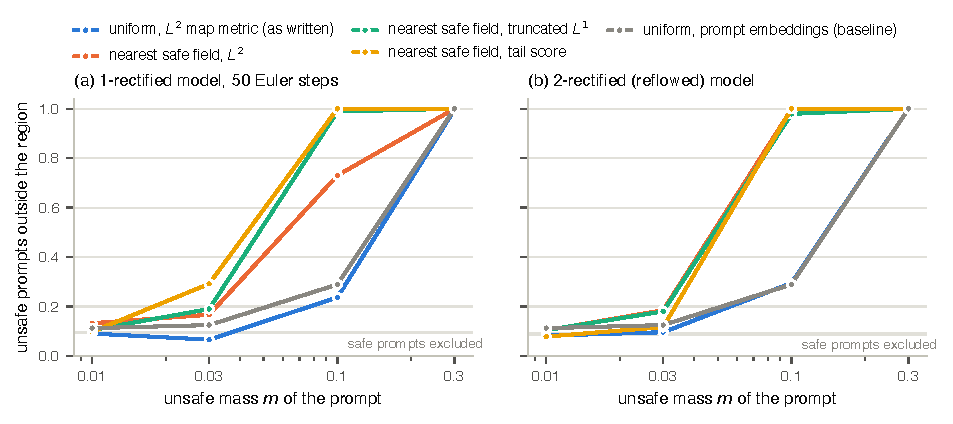
\includegraphics[width=\textwidth]{figures/fig_e1_detection.pdf}
\caption{Step 5, all splits. Exclusion of unsafe prompts against their unsafe mass (means over $100$ splits). The method
as written (blue) and the order-$1$ region on prompt embeddings (grey) coincide on the reflowed model; scoring against
the nearest safe field excludes almost every prompt with $m\ge0.1$ with the $L^1$-type distances (aqua, yellow), and with
$L^2$ (orange) only on the reflowed model. Light grey: fraction of safe test prompts excluded ($1-$coverage).}
\label{fig:e1_detection}
\end{figure}

\paragraph{Step 6: the region in field space, and enforcement.}
A request outside the region is not refused: its field is mixed with a feasible safe field, by bisection on the
mixing weight, until the score reaches the threshold (Proposition~\ref{pr:backoff}). For this model, affine in the prompt,
the mixed field is the field of the mixed prompt (Corollary~\ref{cor:prompt_mixing}). For the running example with $m=0.3$,
both methods mix with the same safe field $c$, a calibration prompt with nearly the same rotation and radius.
Figure~\ref{fig:e1_slice} shows the plane of fields through the unsafe request $u$, the safe field $c$ and the safe anchor $a$ of
Step~4, coloured by the $P(A)$ of their outputs, with the boundary of each region; every point of the plane is the
field of a mixed prompt.
\begin{itemize}
\item Back-off walks from $u$ towards $c$ along the dashed line and stops at the first boundary it meets. It enters the
region as written at $\alpha=\ewAlphaU$, where $P(A)=\ewSlicePAb$ (point~2), and the improved region at $\alpha=\ewAlphaK$, where
$P(A)=\ewSlicePAc$ (point~3).
\item The region as written is one large set, which in this plane contains fields with $P(A)$ up to $\ewSliceMaxU$. The
improved region is a union of small sets around safe fields, the union of balls of Proposition~\ref{pr:truncated}, with
$P(A)\le\ewSliceMaxK$ in this plane. It also leaves out the fields between $c$ and $a$ (point~5): they are not unsafe, but
they produce a smeared ring that no approved prompt asks for.
\item Over $5$ splits and the $100$ prompts with $m=0.3$, enforcement lowers $P(A)$ from $\eonePAAd$ to $\eoneTwoPAasWritten$ as written and to
$\eoneTwoPAtrunc$ with the improved method. It also keeps the outputs closer to the request's safe intent: MMD$^2\times10^3$ to the
$m=0$ target is $\eoneTwoMmdAsWritten$ against $\eoneTwoMmdTrunc$, and $\eoneTwoMmdNone$ without enforcement, because the improved method mixes
with a nearby safe prompt instead of being pulled towards an average one. Safe prompts are altered at the rate
$1-$coverage, without loss of fidelity (Table~\ref{tab:e1_detection}).
\end{itemize}

\begin{figure}[!htbp]
\centering
\includegraphics[width=\textwidth]{figures/fig_e1_slice.pdf}
\caption{Step 6. (a) The plane of fields $c+\alpha(u-c)+\gamma(a-c)$ through the unsafe request $u$ ($m=0.3$), the safe field $c$
towards which both methods back off, and the safe anchor $a$; colour: $P(A)$ of the outputs ($1000$ noises per field).
Blue: boundary of the region as written; aqua: boundary of the improved region; both contain $c$. Dashed arrow:
back-off path. (1)--(6) Outputs ($2000$ noises) of the numbered fields: the request, the two enforced fields, $c$, the
halfway mixture of $c$ and $a$, and $a$.}
\label{fig:e1_slice}
\end{figure}
\FloatBarrier

\paragraph{Step 7: what the certificate says about the enforced field.}
The certificate is a transport argument (Theorem~\ref{th:certificate}, Proposition~\ref{pr:truncated}). Pair each output $Y$ of the
enforced field with the output $Y'$ of a safe field for the same noise. An output in $A$ comes either from a safe output
within $r$ of $A$, or from a pair at least $r$ apart, so $P(Y\in A)\le P(Y'\in A^{+r})+P(\|Y-Y'\|\ge r)$. The first term is measured
on the safe field. The second is bounded by the budget: by $(M+1)\varepsilon/r$ through Markov's inequality for the $L^2$ map
metric, and by $(M+1)\varepsilon\max(1,1/r)$ for the truncated distance. Figure~\ref{fig:e1_certificate} plots both terms and their sum
against $r$; the certificate is the minimum of the sum.
\begin{itemize}
\item \emph{As written} (b), the safe field is the uniform mixture of the anchors, and the budget is large and decays only
like $1/r$. The best bound is $\ewCertU$ (at $r=\ewCertRU$) for an actual $P(A)=\ewCertPAU$: vacuous. Over all fields of the region,
the median Markov bound is $\eoneMarkovMed$.
\item \emph{Improved} (c), the safe field is the nearest anchor and the budget is $\ewCertBudgetK$; the bound is $\ewCertK$ (at
$r=\ewCertRK$) for an actual $P(A)=\ewCertPAK$. Panel (a) shows why it is loose: the noise that the enforced field sends into $A$
is noise that the safe field sends to the inner edge of its blobs, all within $r$ of $A$, so the first term already
covers it, and the bound adds the whole budget on top. The tail score, which counts the redirected noise directly,
certifies $P(A)\le\eoneTwoCertTail$ in median over enforced fields, against $\eoneSafePAA$ for safe prompts.
\item No enforced field violates its certificate on fresh noise (Table~\ref{tab:e1_certificates}). These certificates are
still plug-in, because distances are estimated on $256$ frozen probes. Back-off parks enforced fields on the boundary
of the region, so on fresh noise $\eoneTwoPlugMin$ to $\eoneTwoPlugMax$ of them exceed their budget, by at most a factor $\eoneTwoTruncMaxRatio$ with
the truncated distance, which is bounded, and up to $\eoneTwoLoneMaxRatio$ with $L^1$, which is not. A rigorous certificate uses a
bounded distance and fresh noise: bisect on the frozen probes towards a slightly smaller budget, check the result
once on $L$ fresh probes, and keep it only if the fresh empirical distance plus $\sqrt{\log(1/\delta)/(2L)}$ is within the
budget, falling back to the nearest safe field otherwise. By Hoeffding's inequality (Remark~\ref{rem:mc}) the deployed
field then meets the budget with probability at least $1-\delta$.
\end{itemize}

\begin{figure}[!htbp]
\centering
\includegraphics[width=\textwidth]{figures/fig_e1_certificate.pdf}
\caption{Step 7. (a) Outputs in $A$ of the field enforced by the improved method (red), each joined to the output of the
nearest safe field for the same noise (grey), and $A^{+r}$ at the optimal $r$ (dashed). (b)--(c) The two terms of the
certificate on $P(A)$ and their sum, against the enlargement $r$, for the field enforced as written (relative to the
uniform mixture of the anchors, with Markov's inequality) and for the improved one (relative to the nearest anchor,
truncated distance); dashed: actual $P(A)$ on $2000$ noises.}
\label{fig:e1_certificate}
\end{figure}
\FloatBarrier

\paragraph{Step 8: attacks on the prompt.}
So far the requests were honest: an unsafe mode of a given mass. A white-box attacker instead searches the
embedding space for the prompt with the largest $P(A)$ that the region admits ($12$ random-search runs of $300$ steps,
each starting from an enforced prompt with $m=0.3$). Figure~\ref{fig:e1_attack} shows the worst prompt found in each region
on split $0$.
\begin{itemize}
\item Inside the order-$1$ region built on prompt embeddings, the attacker finds a prompt whose field sends all the
noise into $A$ ($P(A)=\ewAtkPrompt$). Its embedding is closer to an approved embedding ($\ewAtkEmbNear$) than two approved embeddings
typically are to each other (median $\ewAtkEmbMed$), but it is displaced in directions that change the field a lot: its
field scores $\ewAtkScU\varepsilon$ in the field-space region as written and $\ewAtkScK\varepsilon$ in the improved one, which both reject it. The
embedding distance cannot see this, whereas the pull-back metric of Proposition~\ref{pr:mahalanobis}(iii) weighs each
direction of the embedding by its effect on the field.
\item Inside the field-space regions, the worst prompts have $P(A)=\ewAtkWritten$ as written and $\ewAtkImproved$ with the improved
method, below the bound that holds for every field of their region (Table~\ref{tab:e1_certificates}).
\item Over both models, the worst values are $\eoneTwoAttackEU$ and $\eoneTwoAttackEknn$ for the uniform and localised prompt-space regions,
$\eoneTwoAttackUL$ for the field-space region as written, and at most $\eoneTwoAttackLone$ after localisation. On honest unsafe prompts, the
localised prompt-space region does as well as the field-space ones (Table~\ref{tab:e1_detection}): constraining fields rather
than prompts is what protects against adversarial prompts.
\end{itemize}

\begin{figure}[!htbp]
\centering
\includegraphics[width=\textwidth]{figures/fig_e1_attack.pdf}
\caption{Step 8. (a)--(c) Outputs ($1400$ fresh noises) of the prompt with the largest $P(A)$ found by the attack inside the
order-$1$ region on prompt embeddings, inside the field-space region as written, and inside the improved region
(1-rectified model, split $0$). (d) $P(A)$ of the best prompt of each of the $12$ attack runs.}
\label{fig:e1_attack}
\end{figure}
\FloatBarrier

\paragraph{Summary of the results.}
Tables~\ref{tab:e1_detection} and~\ref{tab:e1_certificates} collect the results of the method as written, of its improvements and of the
prompt-space baselines, on both models.
\begin{itemize}
\item Coverage holds for every score (Step~5).
\item The region as written is valid but too wide on a diverse family: its averaged score measures the spread of the
safe fields rather than the request (Steps~4--5).
\item Scoring against the nearest safe field, with a truncated distance, repairs detection, enforcement and the
certificate (Steps~5--7).
\item Field-space regions resist attacks that break prompt-space regions (Step~8).
\item Two limits remain. An unsafe mass smaller than the spread of the nearest safe fields is admitted: exclusion at
$m=0.03$ is at most $\eoneKnnTailb$, and smaller masses need denser safe anchors near the request. And the certificate is
relative to the nearest safe prompt.
\end{itemize}

\begin{table}[!htbp]
\centering
\caption{The method as written against its improvements and against prompt-space regions (means over $5$
splits). Budget: median calibrated threshold of $\sum_iw_id(\bth,\bth_i)$, the $(M+1)\varepsilon$ of
Theorem~\ref{th:certificate}, in the units of each distance. MMD$^2\times10^3$ between the enforced outputs at $m=0.3$
and the $m=0$ target; last column: fraction of safe test prompts altered by enforcement.}
\label{tab:e1_detection}
\small
\begin{tabular}{l c c cc cc c c}
\toprule
& & & \multicolumn{2}{c}{excluded at $m=$} & \multicolumn{2}{c}{enforced $P(A)$, $m=$} & & safe\\
\cmidrule(lr){4-5}\cmidrule(lr){6-7}
score & coverage & budget & $0.03$ & $0.1$ & $0.1$ & $0.3$ & MMD$^2$ & altered\\
\midrule
\inputrows{tables/e1_detection.tex}
\bottomrule
\end{tabular}
\end{table}

\begin{table}[!htbp]
\centering
\caption{Certificates on $P(A)$. Enforced fields ($5$ splits): median bound of each field's certificate,
fields whose $P(A)$ on fresh noise exceeds it, fields whose fresh-noise distance exceeds the budget, and the
a-posteriori bound with the empirical tail of the coupling distance. Attack (split $0$): largest $P(A)$ found
inside the region by random search over embeddings ($12$ starts, $300$ steps), and the bound that holds for
every field of the region.}
\label{tab:e1_certificates}
\small
\begin{tabular}{l c c c c c c}
\toprule
& \multicolumn{4}{c}{enforced fields} & \multicolumn{2}{c}{attack}\\
\cmidrule(lr){2-5}\cmidrule(lr){6-7}
score & bound & violations & over budget & empirical & worst $P(A)$ & bound\\
\midrule
\inputrows{tables/e1_certificates.tex}
\bottomrule
\end{tabular}
\end{table}
\FloatBarrier

\paragraph{The improved method.}
For a prompt with field $\bth$: compute its outputs on $L$ frozen probe noises; score it by the truncated
distance to the nearest safe field, $\min_id_r(\bth,\bth_i)/(M+1)$, calibrated by split conformal prediction as
before; if the score exceeds the threshold, mix the prompt with its nearest safe prompt, by bisection on the
mixing weight (Proposition~\ref{pr:backoff}, Corollary~\ref{cor:prompt_mixing}), and verify the result on fresh probes as
in Step~7. The deployed outputs then satisfy $P(Y\in B)\le P(Y_{i^\star}\in B^{+r})+(M+1)\varepsilon$ for every $B$, relative to the
nearest safe prompt $i^\star$ (Proposition~\ref{pr:truncated}). This keeps the coverage, the order-$1$ Wasserstein structure and
the certificate, and adds locality, robustness to heavy tails and the absence of a Markov factor. Its region is not
convex for multi-step samplers; one-step (straightened) models make it so, at the fidelity cost measured in Step~3.

% =====================================================================================
\section{Static and adaptive regions, on prompts and on fields}\label{sec:e2}
% =====================================================================================

Section~\ref{sec:e1} found, on the two-dimensional toy, that the order-$1$ region as written is valid but too wide, that scoring
a request against the nearest safe field repairs detection, and that regions built on fields resist white-box attacks that
break regions built on prompt embeddings. Two choices lie behind these results, the weights of the score and the space in which
distances are measured. This section separates them, tunes the weights on data disjoint from the evaluation data, and answers
three questions.
\begin{enumerate}[label=(Q\arabic*)]
\item \emph{Weights} (Section~\ref{sec:e2_weights}). Do adaptive weights, which take the transport mass from the approved prompts
closest to the request, beat the static weights of Definition~\ref{def:region}?
\item \emph{Space} (Section~\ref{sec:e2_space}). Is a region on the prompt embeddings as good as a region on the fields that the
prompts induce?
\item \emph{Repairs} (Section~\ref{sec:e2_repairs}). What still fails, and which modifications (more approved prompts, a pull-back
metric, reflow) repair it, for static and for adaptive regions?
\end{enumerate}
Section~\ref{sec:e2_design} describes the design, and Section~\ref{sec:e2_summary} summarises the answers.

\subsection{Design}\label{sec:e2_design}

\paragraph{Task and models.}
The task and the models are those of Section~\ref{sec:e1}. A prompt $z=(\phi,\varrho,m)$ asks for the four-blob ring rotated by
$\phi$ and of radius $\varrho$, with a fraction $m$ of its mass moved into the unsafe disk $A=\{\by:\|\by\|\le0.6\}$. Approved prompts
have $m=0$, $\phi\in[-22.5^\circ,22.5^\circ]$ and $\varrho\in[1.75,2.25]$; an unsafe request has an approved rotation and radius and
$m\in\{0.01,0.03,0.1,0.3\}$. A frozen encoder maps $z$ to $\be\in\RR^{43}$, the normalised $(\phi,\varrho,m)$ followed by $40$ random
Fourier features of them; its third coordinate is $m/0.2$. The model is affine in the embedding, $\bth(\be)=\ba+U\be$
(Definition~\ref{def:prompt}(b)), and is deployed in two versions: the 1-rectified model with $50$ Euler steps, faithful but curved,
and the reflowed model with one Euler step, straight and cheap but less faithful (MMD$^2\times10^3$ to the approved targets:
$\eoneMmdA$ and $\eoneMmdC$; Section~\ref{sec:e1}, Step~3).

\paragraph{Regions.}
A region is given by a distance $d$ between prompts and by weights $w$. A request $\be$ scores $\sum_iw_id(\be,\be_i)$ against $M$
approved prompts $\be_1,\dots,\be_M$, the \emph{anchors}, and is admitted if its score is at most a threshold calibrated on $K$ other
approved prompts (Definition~\ref{def:region} without its factor $1/(M+1)$: the threshold is the budget $(M+1)\varepsilon$ of
Theorem~\ref{th:certificate}). By Lemma~\ref{lem:closed_form}, the score is the cost of the optimal transport plan that moves the mass
$w_i/(M+1)$ from each anchor $i$ to the request. Table~\ref{tab:e2_regions} defines the three distances. The field region uses the
truncated map distance, the most sensitive field distance of Section~\ref{sec:e1}. The pull-back distance is the source-slice
distance $d_0$ between the fields of $\be$ and $\be'$ (Proposition~\ref{pr:mahalanobis}(ii)--(iii)): it weighs each direction of the
embedding by its effect on the field at $t=0$. For a one-step sampler, $d_0$ is the map metric of the deployed sampler
(Corollary~\ref{cor:one_step}(i); numerically, the two agree to a relative error below $10^{-7}$), so the pull-back region of the
reflowed model is a field region computed on the prompts; for the $50$-step 1-rectified model, $d_0$ ignores the later steps.

\begin{table}[!htbp]
\centering
\caption{The three distances between a request $\be$ and an anchor $\be_i$. $T$ and $T_i$ are the noise-to-output maps of the
deployed sampler for $\be$ and $\be_i$, $\bx_0$ ranges over $256$ probe noises shared by all prompts, and $G_0$ is the Gram matrix of
the features at $t=0$ (Proposition~\ref{pr:mahalanobis}(ii)). Field and pull-back regions are computed for one model, named in
parentheses when needed: field (1-rectified), pull-back (reflowed), and so on.}
\label{tab:e2_regions}
\small
\begin{tabular}{l l l l}
\toprule
region & distance $d(\be,\be_i)$ & a score needs & certificate on the outputs\\
\midrule
prompt & $\|\be-\be_i\|$ & the embeddings & none\\
field & $\E\min(\|T(\bx_0)-T_i(\bx_0)\|,1)$ & one run of the sampler & Proposition~\ref{pr:truncated}\\
pull-back & $\|\be-\be_i\|_Q$, $Q=U^\top G_0U$ & the embeddings & Theorem~\ref{th:certificate}, reflowed model only\\
\bottomrule
\end{tabular}
\end{table}

\paragraph{Weights.}
\emph{Static} weights are uniform, $w_i=1/M$. \emph{Adaptive} weights concentrate the transport mass on the anchors closest to the
request. Three families are tuned: Gaussian kernel weights $w_i\propto\exp(-d(\be,\be_i)^2/(2h^2))$, with $h$ equal to $c$ times the
median distance between anchors ($c\to0$ keeps the nearest anchor, $c\to\infty$ gives the static weights); equal weights on the $k$
nearest anchors; and, for field regions, the same kernel in the embedding distance (the prompt-adaptive weights of
Section~\ref{sec:region}). Each weighting is a fixed function of the request given the anchors, so coverage holds for all of them
(Proposition~\ref{pr:coverage}). With $k=1$, the adaptive field region is the improved method of Section~\ref{sec:e1}.

\paragraph{Protocol and metrics.}
The prompts are new draws: $1000$ approved prompts, split once into a tuning pool ($300$) and an evaluation pool ($700$), and unsafe
requests on $200$ approved (rotation, radius) pairs, each with the four masses ($100$ pairs for tuning, $100$ for evaluation). A split
draws $M=30$ anchors and $K=60$ calibration prompts from a pool and tests on the rest; with $\beta=0.1$, the nominal coverage is
$55/61=0.902$. For each region and each $M$, the adaptive family and its parameter maximise the mean exclusion of the four masses
over $50$ splits of the tuning pool; all results come from the evaluation pool, which the tuning never sees.
\begin{itemize}
\item \emph{Coverage}: the fraction of approved test prompts admitted. \emph{Exclusion} at mass $m$: the fraction of unsafe requests
of that mass not admitted. Both are means over $200$ splits ($100$ when $M\ne30$).
\item \emph{Enforcement}: back-off (Proposition~\ref{pr:backoff}) mixes an excluded prompt with its nearest feasible approved prompt
until the score reaches the threshold; for this model, the mixed prompt induces the mixed field (Corollary~\ref{cor:prompt_mixing}).
For the requests with $m=0.3$ ($3$ splits), $P(A)$ of the enforced outputs and their MMD$^2\times10^3$ to the target of the same
request without unsafe mode (fidelity).
\item \emph{Attack}: the white-box search of Section~\ref{sec:e1}, Step~8 ($12$ random-search runs of $300$ steps over embeddings,
from enforced requests with $m=0.3$, one split), for the admitted embedding with the largest $P(A)$, reported on fresh noise.
\end{itemize}
\FloatBarrier

\subsection{Static and adaptive weights}\label{sec:e2_weights}

Table~\ref{tab:e2_summary} collects the results. Coverage lies between $\etCovMin$ and $\etCovMax$ for every region and every weighting
tried (nominal $0.902$), so the regions differ only in what they exclude.

\begin{table}[!htbp]
\centering
\caption{Static and adaptive regions (evaluation pool, $M=30$; regions as in Table~\ref{tab:e2_regions}). Coverage (nominal $0.902$) and
exclusion: means over $200$ splits. Enforcement: $P(A)$ after back-off and MMD$^2\times10^3$ to the target without unsafe mode, for the
requests with $m=0.3$ (means over $3$ splits). Attack: largest $P(A)$ found inside the region ($12$ runs). Adaptive weights: Gaussian
kernel of bandwidth $c$ times the median distance between anchors, in the region's distance or, for ``prompt'', in the embedding
distance. The prompt region does not depend on the model: its two blocks differ only in the outputs it protects.}
\label{tab:e2_summary}
\small
\begin{tabular}{l l c cccc c c c}
\toprule
& & & \multicolumn{4}{c}{excluded at $m=$} & \multicolumn{2}{c}{enforced, $m=0.3$} & attack\\
\cmidrule(lr){4-7}\cmidrule(lr){8-9}
region & weights & coverage & $0.01$ & $0.03$ & $0.1$ & $0.3$ & $P(A)$ & MMD$^2$ & worst $P(A)$\\
\midrule
\inputrows{tables/e2_summary.tex}
\bottomrule
\end{tabular}
\end{table}

\paragraph{Result.}
Adaptive weights exclude far more unsafe requests than static ones, in both spaces (Figure~\ref{fig:e2_detection}(a)). At $m=0.1$,
exclusion rises from $\etExESc$ to $\etExEAc$ for the prompt region and from $\etExFSc$ to $\etExFAc$ for the field region. Smaller masses
remain hard: at $m=0.03$ the adaptive regions exclude $\etExEAb$ and $\etExFAb$, and at $m=0.01$ every region excludes barely more unsafe
requests than approved prompts (Section~\ref{sec:e2_repairs}).

\begin{figure}[!htbp]
\centering
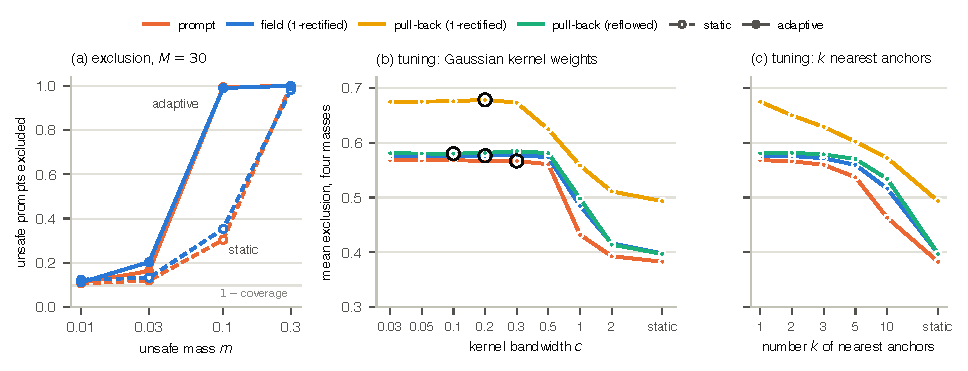
\includegraphics[width=\textwidth]{figures/fig_e2_detection.pdf}
\caption{(a) Exclusion of unsafe requests against their mass, for the prompt and field regions (1-rectified model) with static
(dashed) and adaptive (solid) weights; means over $200$ evaluation splits, $M=30$. (b)--(c) Tuning of the adaptive weights: mean
exclusion over the four masses against the bandwidth $c$ of Gaussian kernel weights, relative to the median distance between
anchors (b), and against the number $k$ of nearest anchors given equal weights (c). The last point of each curve is the static
region; circles mark the weights chosen on the tuning pool; all curves are measured on the evaluation pool.}
\label{fig:e2_detection}
\end{figure}

\paragraph{Mechanism.}
Static weights take the same mass from every anchor, whatever its rotation, so the score averages distances dominated by the
rotation spread of the approved family; by Proposition~\ref{pr:geometry}(iii), a static budget is at least half the mean distance
between anchors, whatever the request. Figure~\ref{fig:e2_mechanism} follows one request (rotation $10^\circ$, radius $2$, $m=0.1$). With
static weights it scores $\etScEstatic\varepsilon$ (prompt) and $\etScFstatic\varepsilon$ (field), and is admitted (panels (a) and (c)). The tuned
adaptive weights take $\etWEtopthree$ (prompt) and $\etWFtopthree$ (field) of the mass from the three nearest anchors, which nearly share the
request's rotation and radius, so the score becomes a distance to these neighbours and the request is excluded ($\etScEadaptive\varepsilon$
and $\etScFadaptive\varepsilon$; panels (b) and (d)). Over all requests (bottom row), static regions admit a dome of unsafe requests above
the approved rotations, up to $m=\etMapMaxEstatic$ (prompt) and $m=\etMapMaxTRstatic$ (field); adaptive regions admit a thin band, up to
$m=\etMapMaxEadaptive$ and $m=\etMapMaxTRadaptive$.

\begin{figure}[!htbp]
\centering
\includegraphics[width=\textwidth]{figures/fig_e2_mechanism.pdf}
\caption{Why adaptive weights exclude more. Each column is one region (1-rectified model, evaluation split $0$). Top: the optimal
transport plan of the order-$1$ score for one unsafe request (star: rotation $10^\circ$, radius $2$, $m=0.1$); each disc is an anchor,
placed by its rotation and radius, with an area proportional to its weight $w_i$, the mass that the plan moves from it to the
request; scores are in units of the threshold $\varepsilon$. Bottom: admission maps for requests of radius $2$ (admitted requests shaded;
black segment: approved requests; star: the request of the top row; ticks: rotations of the $30$ anchors, of various radii).}
\label{fig:e2_mechanism}
\end{figure}

\paragraph{Tuning.}
The best adaptive weights are local (Figure~\ref{fig:e2_detection}(b)--(c)). In every space, mean exclusion is flat from $c=0.03$,
where the kernel keeps only the nearest anchor, to $c=0.3$, and falls for wider kernels; with equal weights on the $k$ nearest
anchors, it is highest for $k\le2$. Spreading the mass lets the spread of the family back into the score. The weights chosen on the
tuning pool are within $\etTuneRegret$ of the best on the evaluation pool, and the nearest anchor alone is within $\etNearGap$: tuning
confirms the improved method of Section~\ref{sec:e1} rather than improving on it.

\paragraph{Take-away.}
A static region measures the spread of the approved family, in either space. Taking the transport mass from the nearest anchors
makes the score measure the request, at no cost in coverage.
\FloatBarrier

\subsection{Prompt space and field space}\label{sec:e2_space}

The requests above are \emph{honest}: prompts $z$ passed through the encoder. On them the two spaces perform alike; two departures
from this setting separate them.

\paragraph{Honest requests.}
The prompt and field regions exclude as many unsafe requests, static or adaptive (Figure~\ref{fig:e2_detection}(a)), and both enforce
well. For the requests with $m=0.3$, which the 1-rectified model serves with $P(A)=\etPoolPAOne$, back-off brings $P(A)$ to $\etEnfOneEA$
with the adaptive prompt region and $\etEnfOneFA$ with the adaptive field region ($\etEnfOneES$ and $\etEnfOneFS$ with static weights;
Figure~\ref{fig:e2_attack}(b)). The reason is the encoder: as the third coordinate of the embedding is $m/0.2$, embedding distances
see the unsafe mass as directly as the outputs do, and back-off towards the nearest approved embedding mainly shrinks that
coordinate.

\paragraph{White-box attack.}
An attacker who controls the embedding is not bound by the encoder. Inside the prompt regions of the 1-rectified model, the attack
finds admitted embeddings with $P(A)$ up to $\etAtkOneES$ (static) and $\etAtkOneEA$ (adaptive; Figure~\ref{fig:e2_attack}(a)): they are
close to approved embeddings in directions that change the field strongly, which the Euclidean distance does not weigh. Inside the
field regions, the worst values are $\etAtkOneFS$ (static) and $\etAtkOneFA$ (adaptive). Adaptive weights buy robustness only in a space
that sees the field.

\begin{figure}[!htbp]
\centering
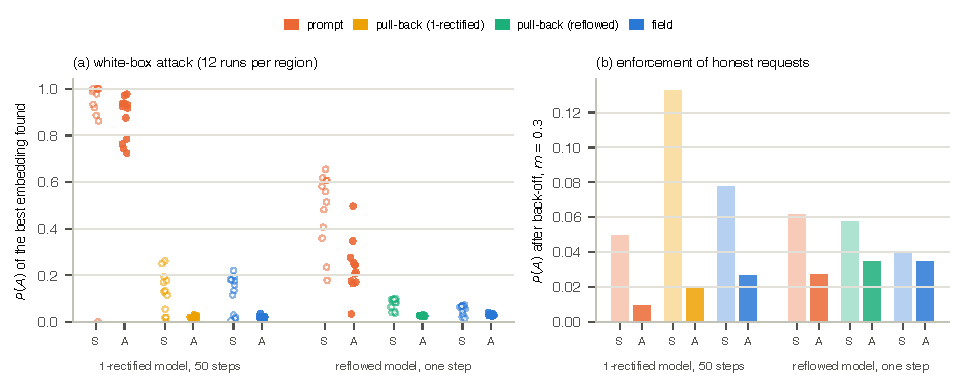
\includegraphics[width=\textwidth]{figures/fig_e2_attack.pdf}
\caption{Regions against an attacker and on honest requests. (a) White-box attack: $P(A)$, on fresh noise, of the best embedding
found by each of $12$ random-search runs inside each region (S: static; A: adaptive weights). (b) Enforcement: $P(A)$ after back-off for
the requests with $m=0.3$ (means over $3$ splits). Left groups: regions protecting the 1-rectified model ($50$ Euler steps); right
groups: regions protecting the reflowed model sampled in one step, whose pull-back metric is its field metric.}
\label{fig:e2_attack}
\end{figure}

\paragraph{Nuisance wording.}
Real prompts also differ in wording that moves the embedding without changing the request. To model this, each prompt receives a
token $s\sim\mathcal U[-1,1]$, encoded in $10$ extra coordinates scaled by $\lambda$, which leaves the target unchanged, and the
1-rectified model is refitted on prompts with random tokens. It learns to ignore the token: its fidelity is that of the model
without token (MMD$^2\times10^3=\etNuMmd$ against $\eoneMmdA$; $P(A)=\etNuPAd$ against $\eonePAAd$ at $m=0.3$), and two tokens of one
request give outputs at truncated distance $\etNuSame$ (median), against $\etNuPairs$ for two approved requests. Least squares is
invariant to the scale of the token coordinates, so only the prompt region depends on $\lambda$ (Figure~\ref{fig:e2_nuisance}). As $\lambda$
grows, its nearest anchors become those with a similar token rather than a similar request: adaptive exclusion at $m=0.1$ falls
from $\etNuEzeroA$ without token to $\etNuEtwoA$ at $\lambda=2$ and $\etNuEfourA$ at $\lambda=4$ (static: $\etNuEzeroS$ to $\etNuEfourS$), while the
adaptive field region keeps $\etNuFA$. Coverage stays between $\etNuCovMin$ and $\etNuCovMax$.

\begin{figure}[!htbp]
\centering
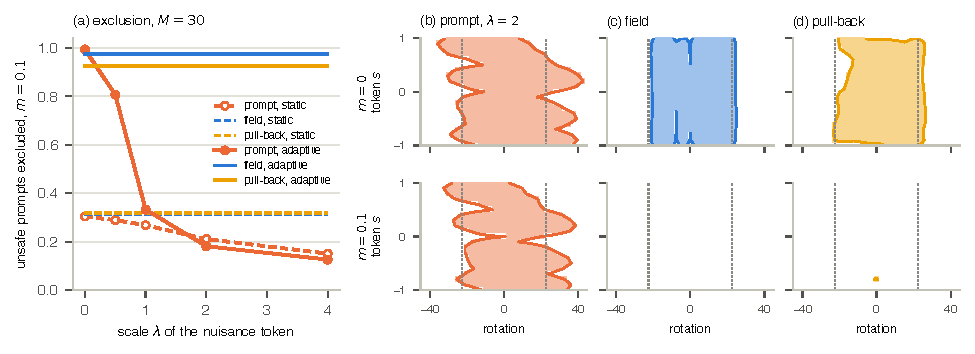
\includegraphics[width=\textwidth]{figures/fig_e2_nuisance.pdf}
\caption{Prompts with a nuisance token $s$, encoded in $10$ extra embedding coordinates scaled by $\lambda$ and ignored by the refitted
1-rectified model. (a) Exclusion at $m=0.1$ against $\lambda$ ($M=30$, $200$ splits); the field and pull-back regions of this model do not
depend on $\lambda$. (b)--(d) Admission maps of the adaptive regions over rotation and token, for requests of radius $2$ with $m=0$ (top)
and $m=0.1$ (bottom); dotted lines: approved rotations. The prompt region admits unsafe requests for many tokens; the field region
admits by rotation alone, and no request with $m=0.1$.}
\label{fig:e2_nuisance}
\end{figure}

\paragraph{Take-away.}
A prompt region is only as good as the encoder: it matches a field region when the embedding exposes the unsafe content, and
fails, static or adaptive, under attacks on the embedding or wording that the model ignores. A field region resists both.

\subsection{Failures and modifications}\label{sec:e2_repairs}

Four failures remain. Each is given below with its cause and a modification; Table~\ref{tab:e2_repairs} reports the effect of each
modification on the static and on the adaptive regions.

\begin{table}[!htbp]
\centering
\caption{Effect of each modification on the static and on the adaptive regions (evaluation pool; before $\to$ after). Attack: largest
$P(A)$ found inside the region; MMD$^2\times10^3$: fidelity after enforcement of the requests with $m=0.3$. The pull-back rows replace the
prompt region by the pull-back region of the same model; the token row uses the refitted model of Section~\ref{sec:e2_space} with
$\lambda=4$. The reflow rows replace the field region of the 1-rectified model by that of the reflowed model sampled in one step.}
\label{tab:e2_repairs}
\small
\begin{tabular}{l l l c c}
\toprule
modification & setting & measure & static & adaptive\\
\midrule
$240$ anchors instead of $30$ & prompt & excluded at $m=0.03$ & $\etDensUEA\to\etDensUEB$ & $\etDensEA\to\etDensEB$\\
& field (1-rectified) & & $\etDensUFA\to\etDensUFB$ & $\etDensFA\to\etDensFB$\\
\midrule
pull-back metric & 1-rectified & worst attack $P(A)$ & $\etAtkOneES\to\etAtkOnePBS$ & $\etAtkOneEA\to\etAtkOnePBA$\\
& 1-rectified, token & excluded at $m=0.1$ & $\etNuEfourS\to\etNuPS$ & $\etNuEfourA\to\etNuPA$\\
& reflowed & worst attack $P(A)$ & $\etAtkTwoES\to\etAtkTwoPBS$ & $\etAtkTwoEA\to\etAtkTwoPBA$\\
\midrule
reflow, one step & field & excluded at $m=0.1$ & $\etExFSc\to\etExTSc$ & $\etExFAc\to\etExTAc$\\
& & worst attack $P(A)$ & $\etAtkOneFS\to\etAtkTwoFS$ & $\etAtkOneFA\to\etAtkTwoFA$\\
& & MMD$^2$ after enforcement & $\etMmdOneFS\to\etMmdTwoFS$ & $\etMmdOneFA\to\etMmdTwoFA$\\
\bottomrule
\end{tabular}
\end{table}

\paragraph{Static regions are too wide, and more anchors do not help.}
A static budget is set by the spread of the approved family (Proposition~\ref{pr:geometry}(iii)), not by the number of anchors: from
$30$ to $240$ anchors it goes from $\etEpsUEA$ to $\etEpsUEB$ (prompt) and from $\etEpsUFA$ to $\etEpsUFB$ (field), and exclusion barely moves
(Figure~\ref{fig:e2_density}). Adaptive weights are the main repair. Reflow with one-step sampling also helps the static field region,
because it shrinks the spread more than the effect of an unsafe mode: the one-step outputs are smeared along the ring
(Figure~\ref{fig:e1_time}), so the mean field distance between approved prompts falls from $\etSpreadOne$ to $\etSpreadTwo$, while the median
distance from a request with $m=0.1$ to its nearest approved prompt only falls from $\etDispOne$ to $\etDispTwo$.

\paragraph{Adaptive regions are only as fine as the anchors.}
An adaptive budget is set by the distance from an approved prompt to its nearest anchors, so an unsafe mode that moves the outputs
by less is admitted, as $m=0.03$ is with $30$ anchors. From $30$ to $240$ anchors, this budget falls from $\etEpsEA$ to $\etEpsEB$ (prompt)
and from $\etEpsFA$ to $\etEpsFB$ (field), and almost every request with $m=0.03$ is excluded (Figure~\ref{fig:e2_density}(a)); $m=0.01$
needs denser anchors still (at most a fraction $\etDensOneP$ is excluded with $240$ anchors). With nearly nearest-neighbour weights, an
adaptive region is close to a union of small balls around the anchors: it is not convex, and it is enforced by back-off rather than
by projection.

\begin{figure}[!htbp]
\centering
\includegraphics[width=\textwidth]{figures/fig_e2_density.pdf}
\caption{Exclusion of small unsafe masses against the number $M$ of anchors (evaluation pool, $K=60$, adaptive weights tuned for each
$M$); dashed: static; solid: adaptive. The static budget is set by the spread of the approved family and does not shrink with $M$; the
adaptive budget shrinks with the distance to the nearest anchors.}
\label{fig:e2_density}
\end{figure}

\paragraph{Prompt regions do not see the model.}
The pull-back metric weighs each direction of the embedding by its effect on the field at $t=0$, so it ignores what the model
ignores, without simulation. With adaptive weights it caps the attack at a few percent on both models and keeps most of the
detection with nuisance tokens (Table~\ref{tab:e2_repairs}). On the 1-rectified model, however, it measures the field at $t=0$, not the
$50$-step sampler: its certificate pays straightness defects of order $\eoneZetaA$ (Corollary~\ref{cor:one_step}(ii)) and is vacuous, and
with static weights it leaves $P(A)=\etEnfOnePBS$ after enforcement. Its detection, the strongest of all regions ($\etExSAb$ at $m=0.03$,
adaptive), rests on what the fitted field leaks at $t=0$: the exact field at $t=0$ depends on the target only through its mean
(Lemma~\ref{lem:time}(iii)), which the unsafe mode leaves unchanged.

\paragraph{Field regions of a curved model are costly.}
On the 1-rectified model, each field score runs the $50$-step sampler on the $256$ probes, back-off repeats it about $18$ times, and
the region is not convex. Reflow with one-step sampling (Remark~\ref{rem:reflow}) removes these costs: the pull-back metric of the
reflowed one-step model \emph{is} the map metric of its deployed sampler (Corollary~\ref{cor:one_step}(i)). Its region lives on the
prompts, needs no simulation, is convex with static weights (Proposition~\ref{pr:geometry}(i)) and keeps the certificate of
Theorem~\ref{th:certificate}. It detects as well as the field regions (Table~\ref{tab:e2_summary}), gains as much from denser anchors
(Figure~\ref{fig:e2_density}) and resists the attack, unlike the Euclidean prompt region of the same model (Table~\ref{tab:e2_repairs}).
The price is the fidelity of one-step sampling (MMD$^2\times10^3=\eoneMmdC$ on approved prompts, against $\eoneMmdA$), which
enforcement inherits (Table~\ref{tab:e2_summary}).
\FloatBarrier

\subsection{Summary}\label{sec:e2_summary}

On this toy, the weights decide detection and the space decides robustness.
(Q1) Static regions are valid but too wide in every space, because their budget is set by the spread of the approved family.
Adaptive weights that take the transport mass from the nearest anchors repair detection at no cost in coverage, and resolve smaller
unsafe masses as the anchors become denser.
(Q2) Prompt regions match field regions only while the encoder exposes the unsafe content; field regions resist attacks on the
embedding and wording that the model ignores.
(Q3) The best configuration is an adaptive region on a field metric. For a model reflowed and sampled in one step, that metric is
the pull-back metric on the prompts, which is cheap and certified, at the fidelity cost of one-step sampling.

% =====================================================================================
\section{Status and next steps}\label{sec:next}
% =====================================================================================

Proved: coverage of the field of a new approved prompt (Proposition~\ref{pr:coverage}); convexity and
second-order cone formulations for Mahalanobis distances (Propositions~\ref{pr:geometry} and~\ref{pr:projection});
enforcement as a mixture of fields, and as prompt mixing for models affine in the prompt
(Proposition~\ref{pr:projection}(iii), Corollary~\ref{cor:prompt_mixing}); an output certificate for every enforced field,
without Gr\"onwall factor (Theorem~\ref{th:certificate}), convex for one-step samplers and paying straightness
defects otherwise (Corollary~\ref{cor:one_step}), and without Markov factor for the localised truncated distance
(Proposition~\ref{pr:truncated}). Tested: on the POC toy, the off-policy/on-policy gap and the path-divergence
certificates (Section~\ref{sec:evidence}); on a prompt-conditioned toy, coverage, the role of time, prompt mixing, the
failure of the region as written on a diverse family, its repair by localisation and truncation, and the
robustness of field-space regions to white-box attacks on the prompt (Section~\ref{sec:e1}); and, with tuning separated
from evaluation, that adaptive weights beat static ones in every space and need denser anchors for small unsafe masses,
that prompt-space regions match field-space ones on honest prompts only when the encoder exposes the unsafe content,
and that a pull-back metric of a one-step reflowed model turns the prompt region into the field region
(Section~\ref{sec:e2}). The central tension
remains between convexity, which needs a fixed reference law, and safety, which needs each field to be
evaluated where it sends the noise; one-step samplers resolve it, at a cost in fidelity.

Next: Monte Carlo margins that make the deployed certificate rigorous; the choice of anchors when safe
prompts are many, since the budget is set by the spread of the nearest safe fields; then a forbidden class
with class-conditional rectified flows on MNIST and CIFAR-10, and text-to-image generation with the
truncated map distance in the feature space of an image encoder $\chi$ (POC Section~10), always evaluated
against white-box attacks on the prompt.

\appendix
% =====================================================================================
\section{Stochastic samplers and path divergences}\label{app:sde}
% =====================================================================================

With $\TV$, $\KL$ and $\kl$ as in Definition~\ref{def:divergences}, we restate the POC results on stochastic samplers in the
notation of this note; the facts on divergences used below are listed after that definition.

\begin{definition}[SDE chain]\label{def:sde}
For $\eta>0$ and the grid of Definition~\ref{def:sampler}, the SDE chain of $\bth$ is $X_0\sim\mu_0$ and
$X_{k+1}=X_k+h_k[(1+\eta t_k)\Phi(X_k,t_k)\bth-\eta X_k]+\sigma_k\bxi_k$, $\sigma_k^2=2\eta(1-t_k)h_k$, $k=0,\dots,J-1$, with
$\bxi_k$ i.i.d.\ $\cN(0,I_n)$ independent of $X_0$; $P^{\bth}$ is the law of $(X_0,\dots,X_J)$. With $\Phi\bth$ replaced by $\vstar_p$, its
continuous-time limit has, formally, the marginals of the interpolation path (POC Lemma~3,
\citealt{albergo2025stochastic}); this is not used below.
\end{definition}

\begin{lemma}[Path divergence]\label{lem:chain_kl}
$\KL(P^{\bth}\|P^{\bth'})=\frac12(\bth-\bth')^\top G_{\KL}(\bth)(\bth-\bth')$, where
$G_{\KL}(\bth)=\sum_{k=0}^{J-1}\omega_k\E_{P^{\bth}}[\Phi(X_k,t_k)^\top\Phi(X_k,t_k)]$ and $\omega_k=\frac{h_k(1+\eta t_k)^2}{2\eta(1-t_k)}$.
\end{lemma}
\textit{Proof:}
$\sigma_k>0$ because $t_k<1$ for $k\le J-1$, and each $X_k$ has a finite second moment by linear growth.
Both chains are Markov with the same initial law and Gaussian kernels of covariance $\sigma_k^2I_n$
whose means differ by $h_k(1+\eta t_k)\Phi(X_k,t_k)(\bth-\bth')$. The chain rule for relative entropy
\citep[Thm.~2.5.3]{cover2006elements} sums, in expectation under $P^{\bth}$, the divergences between these Gaussian kernels,
$\|h_k(1+\eta t_k)\Phi(X_k,t_k)(\bth-\bth')\|^2/(2\sigma_k^2)=\frac{\omega_k}{2}\|\Phi(X_k,t_k)(\bth-\bth')\|^2$ (the Gaussian formula after
Definition~\ref{def:divergences}).
\hfill$\square$

The forward cost $\KL(P^{\bth_i}\|P^{\bth})$ uses the Gram matrix of the safe chain and is convex in $\bth$; the
reverse cost $\KL(P^{\bth}\|P^{\bth_i})$ uses that of the candidate and is not.

\begin{proposition}[Certificates and the direction of the divergence]\label{pr:sde_cert}
Let $\bar P_w=\sum_iw_iP^{\bth_i}$.
(i) If $\frac{1}{M+1}\sum_iw_i\KL(P^{\bth_i}\|P^{\bth})\le\varepsilon$, then
$\TV(P^{\bth},\bar P_w)\le\min\{((M+1)\varepsilon/2)^{1/2},(1-e^{-(M+1)\varepsilon})^{1/2}\}$.
(ii) If $\frac{1}{M+1}\sum_iw_i\KL(P^{\bth}\|P^{\bth_i})\le\varepsilon$, then for every event $A$ with $q=\bar P_w(A)\in(0,1)$,
\[
P^{\bth}(A)\le\sup\{x\in[q,1]:\kl(x\|q)\le(M+1)\varepsilon\}\le\frac{(M+1)\varepsilon+\log2}{\log(1/q)}.
\]
(iii) If $P'=(1-m)P+mQ$ with $m\in[0,1)$, then $\KL(P\|P')\le\log\frac{1}{1-m}$. If moreover $Q(A)=1$ for an
event $A$ with $q=P(A)\in(0,1)$ and $m\ge q$, then $\KL(P'\|P)\ge m\log\frac mq-m$.
\end{proposition}
\textit{Proof:}
(i) By joint convexity of the relative entropy \citep[Thm.~2.7.2]{cover2006elements},
$\KL(\bar P_w\|P^{\bth})\le\sum_iw_i\KL(P^{\bth_i}\|P^{\bth})\le(M+1)\varepsilon$; apply Pinsker's inequality
\citep[Lemma~2.5]{tsybakov2009introduction} and the Bretagnolle--Huber inequality
\citep{bretagnolle1979estimation,canonne2022short}.
(ii) Likewise, by convexity in the second argument, $\KL(P^{\bth}\|\bar P_w)\le(M+1)\varepsilon$. By data
processing through $\mathbbm 1_A$ (after Definition~\ref{def:divergences}), $\kl(P^{\bth}(A)\|q)\le(M+1)\varepsilon$: either $P^{\bth}(A)\le q$, or $P^{\bth}(A)$ belongs to the
set whose supremum is taken. For the second bound, every $x$ in that set satisfies
$x\log\frac1q-\log2\le\kl(x\|q)\le(M+1)\varepsilon$, because $\kl(x\|q)=x\log\frac1q+(1-x)\log\frac1{1-q}-\mathrm h(x)$ with the binary
entropy $\mathrm h(x)\le\log2$.
(iii) $P\le\frac{1}{1-m}P'$, so $\frac{dP}{dP'}\le\frac1{1-m}$ and $\KL(P\|P')\le\log\frac1{1-m}$. Let $x=P'(A)=(1-m)q+m$, so
$x\ge m\ge q$. Data processing and $\log\frac1{1-q}\ge0$ give $\KL(P'\|P)\ge x\log\frac xq+(1-x)\log(1-x)\ge x\log\frac xq-x$,
since $\log(1-x)\ge-\frac{x}{1-x}$ for $x<1$; and $x\mapsto x\log\frac xq-x$ has derivative $\log\frac xq\ge0$ on $[q,1]$.
\hfill$\square$

Item (iii) is the formal reason for the gap of Section~\ref{sec:evidence}: a forward cost charges at most
$\log\frac1{1-m}\approx m$ for an unsafe mode of mass $m$, whatever its rarity $q$ under the safe samplers, while
the reverse cost grows like $m\log(m/q)$.

\bibliographystyle{informs2014}
\bibliography{refs}

\end{document}
